% Options for packages loaded elsewhere
\PassOptionsToPackage{unicode}{hyperref}
\PassOptionsToPackage{hyphens}{url}
%
\documentclass[
]{article}
\usepackage{amsmath,amssymb}
\usepackage{iftex}
\ifPDFTeX
  \usepackage[T1]{fontenc}
  \usepackage[utf8]{inputenc}
  \usepackage{textcomp} % provide euro and other symbols
\else % if luatex or xetex
  \usepackage{unicode-math} % this also loads fontspec
  \defaultfontfeatures{Scale=MatchLowercase}
  \defaultfontfeatures[\rmfamily]{Ligatures=TeX,Scale=1}
\fi
\usepackage{lmodern}
\ifPDFTeX\else
  % xetex/luatex font selection
\fi
% Use upquote if available, for straight quotes in verbatim environments
\IfFileExists{upquote.sty}{\usepackage{upquote}}{}
\IfFileExists{microtype.sty}{% use microtype if available
  \usepackage[]{microtype}
  \UseMicrotypeSet[protrusion]{basicmath} % disable protrusion for tt fonts
}{}
\makeatletter
\@ifundefined{KOMAClassName}{% if non-KOMA class
  \IfFileExists{parskip.sty}{%
    \usepackage{parskip}
  }{% else
    \setlength{\parindent}{0pt}
    \setlength{\parskip}{6pt plus 2pt minus 1pt}}
}{% if KOMA class
  \KOMAoptions{parskip=half}}
\makeatother
\usepackage{xcolor}
\usepackage[margin=1in]{geometry}
\usepackage{color}
\usepackage{fancyvrb}
\newcommand{\VerbBar}{|}
\newcommand{\VERB}{\Verb[commandchars=\\\{\}]}
\DefineVerbatimEnvironment{Highlighting}{Verbatim}{commandchars=\\\{\}}
% Add ',fontsize=\small' for more characters per line
\usepackage{framed}
\definecolor{shadecolor}{RGB}{248,248,248}
\newenvironment{Shaded}{\begin{snugshade}}{\end{snugshade}}
\newcommand{\AlertTok}[1]{\textcolor[rgb]{0.94,0.16,0.16}{#1}}
\newcommand{\AnnotationTok}[1]{\textcolor[rgb]{0.56,0.35,0.01}{\textbf{\textit{#1}}}}
\newcommand{\AttributeTok}[1]{\textcolor[rgb]{0.13,0.29,0.53}{#1}}
\newcommand{\BaseNTok}[1]{\textcolor[rgb]{0.00,0.00,0.81}{#1}}
\newcommand{\BuiltInTok}[1]{#1}
\newcommand{\CharTok}[1]{\textcolor[rgb]{0.31,0.60,0.02}{#1}}
\newcommand{\CommentTok}[1]{\textcolor[rgb]{0.56,0.35,0.01}{\textit{#1}}}
\newcommand{\CommentVarTok}[1]{\textcolor[rgb]{0.56,0.35,0.01}{\textbf{\textit{#1}}}}
\newcommand{\ConstantTok}[1]{\textcolor[rgb]{0.56,0.35,0.01}{#1}}
\newcommand{\ControlFlowTok}[1]{\textcolor[rgb]{0.13,0.29,0.53}{\textbf{#1}}}
\newcommand{\DataTypeTok}[1]{\textcolor[rgb]{0.13,0.29,0.53}{#1}}
\newcommand{\DecValTok}[1]{\textcolor[rgb]{0.00,0.00,0.81}{#1}}
\newcommand{\DocumentationTok}[1]{\textcolor[rgb]{0.56,0.35,0.01}{\textbf{\textit{#1}}}}
\newcommand{\ErrorTok}[1]{\textcolor[rgb]{0.64,0.00,0.00}{\textbf{#1}}}
\newcommand{\ExtensionTok}[1]{#1}
\newcommand{\FloatTok}[1]{\textcolor[rgb]{0.00,0.00,0.81}{#1}}
\newcommand{\FunctionTok}[1]{\textcolor[rgb]{0.13,0.29,0.53}{\textbf{#1}}}
\newcommand{\ImportTok}[1]{#1}
\newcommand{\InformationTok}[1]{\textcolor[rgb]{0.56,0.35,0.01}{\textbf{\textit{#1}}}}
\newcommand{\KeywordTok}[1]{\textcolor[rgb]{0.13,0.29,0.53}{\textbf{#1}}}
\newcommand{\NormalTok}[1]{#1}
\newcommand{\OperatorTok}[1]{\textcolor[rgb]{0.81,0.36,0.00}{\textbf{#1}}}
\newcommand{\OtherTok}[1]{\textcolor[rgb]{0.56,0.35,0.01}{#1}}
\newcommand{\PreprocessorTok}[1]{\textcolor[rgb]{0.56,0.35,0.01}{\textit{#1}}}
\newcommand{\RegionMarkerTok}[1]{#1}
\newcommand{\SpecialCharTok}[1]{\textcolor[rgb]{0.81,0.36,0.00}{\textbf{#1}}}
\newcommand{\SpecialStringTok}[1]{\textcolor[rgb]{0.31,0.60,0.02}{#1}}
\newcommand{\StringTok}[1]{\textcolor[rgb]{0.31,0.60,0.02}{#1}}
\newcommand{\VariableTok}[1]{\textcolor[rgb]{0.00,0.00,0.00}{#1}}
\newcommand{\VerbatimStringTok}[1]{\textcolor[rgb]{0.31,0.60,0.02}{#1}}
\newcommand{\WarningTok}[1]{\textcolor[rgb]{0.56,0.35,0.01}{\textbf{\textit{#1}}}}
\usepackage{graphicx}
\makeatletter
\def\maxwidth{\ifdim\Gin@nat@width>\linewidth\linewidth\else\Gin@nat@width\fi}
\def\maxheight{\ifdim\Gin@nat@height>\textheight\textheight\else\Gin@nat@height\fi}
\makeatother
% Scale images if necessary, so that they will not overflow the page
% margins by default, and it is still possible to overwrite the defaults
% using explicit options in \includegraphics[width, height, ...]{}
\setkeys{Gin}{width=\maxwidth,height=\maxheight,keepaspectratio}
% Set default figure placement to htbp
\makeatletter
\def\fps@figure{htbp}
\makeatother
\setlength{\emergencystretch}{3em} % prevent overfull lines
\providecommand{\tightlist}{%
  \setlength{\itemsep}{0pt}\setlength{\parskip}{0pt}}
\setcounter{secnumdepth}{-\maxdimen} % remove section numbering
\usepackage{booktabs}
\usepackage{longtable}
\usepackage{array}
\usepackage{multirow}
\usepackage{wrapfig}
\usepackage{float}
\usepackage{colortbl}
\usepackage{pdflscape}
\usepackage{tabu}
\usepackage{threeparttable}
\usepackage{threeparttablex}
\usepackage[normalem]{ulem}
\usepackage{makecell}
\usepackage{xcolor}
\ifLuaTeX
  \usepackage{selnolig}  % disable illegal ligatures
\fi
\IfFileExists{bookmark.sty}{\usepackage{bookmark}}{\usepackage{hyperref}}
\IfFileExists{xurl.sty}{\usepackage{xurl}}{} % add URL line breaks if available
\urlstyle{same}
\hypersetup{
  pdftitle={TMA4315 Generalized linear models H2018},
  pdfauthor={Mette Langaas, Department of Mathematical Sciences, NTNU - with contributions from Øyvind Bakke, Thea Bjørnland and Ingeborg Hem},
  hidelinks,
  pdfcreator={LaTeX via pandoc}}

\title{TMA4315 Generalized linear models H2018}
\usepackage{etoolbox}
\makeatletter
\providecommand{\subtitle}[1]{% add subtitle to \maketitle
  \apptocmd{\@title}{\par {\large #1 \par}}{}{}
}
\makeatother
\subtitle{Module 3: BINARY REGRESSION}
\author{Mette Langaas, Department of Mathematical Sciences, NTNU - with
contributions from Øyvind Bakke, Thea Bjørnland and Ingeborg Hem}
\date{13.09 and 20.09 {[}PL{]}, 14.09 and 21.09 {[}IL{]}}

\begin{document}
\maketitle

{
\setcounter{tocdepth}{2}
\tableofcontents
}
(Latest changes: 09.11: clarified one sentence on the devianc. 23.09:
score test moved to M4. 20.09: typos, and added solutions to Qs in
class. 18.09: typos and added sententence ILw2Problem3c. 16.09: edited
and added material for week 2, 13.09 moved material not lectured to
after the ILw1, and added one sentence to Problem 5 ILw1.)

\hypertarget{overview}{%
\section{Overview}\label{overview}}

\hypertarget{learning-material}{%
\subsection{Learning material}\label{learning-material}}

\begin{itemize}
\tightlist
\item
  Textbook: Fahrmeir et al (2013): Chapter 2.3, 5.1, B4.1-3
\item
  \href{https://www.math.ntnu.no/emner/TMA4315/2018h/TMA4315M3H20180913.pdf}{Classnotes
  13.09.2018}
\item
  \href{https://www.math.ntnu.no/emner/TMA4315/2018h/TMA4315M3H20180920.pdf}{Classnotes
  20.09.2018}
\end{itemize}

\begin{center}\rule{0.5\linewidth}{0.5pt}\end{center}

\hypertarget{topics}{%
\subsection{Topics}\label{topics}}

\hypertarget{first-week}{%
\subsubsection{\texorpdfstring{\protect\hyperlink{firstweek}{First
week}}{First week}}\label{first-week}}

\begin{itemize}
\tightlist
\item
  aim of binary regression
\item
  how to model a binary response
\item
  three ingredients of a GLM model
\item
  the logit model: logistic regression
\item
  interpreting the logit model - with odds
\item
  grouped vs.~individual data
\item
  parameter estimation with maximum likelihood

  \begin{itemize}
  \tightlist
  \item
    likelihood, log-likelihood,
  \item
    score function
  \end{itemize}
\end{itemize}

Jump to \protect\hyperlink{ILw1}{interactive lecture (week 1)}

\begin{center}\rule{0.5\linewidth}{0.5pt}\end{center}

\hypertarget{second-week}{%
\subsubsection{\texorpdfstring{\protect\hyperlink{secondweek}{Second
week}}{Second week}}\label{second-week}}

\begin{itemize}
\tightlist
\item
  Parameter estimation

  \begin{itemize}
  \tightlist
  \item
    score function- and mean and covariance thereof,
  \item
    observed and expected information matrix
  \end{itemize}
\item
  comparison with the normal distribution - score function and Fisher
  information
\item
  exponential family and canonical link
\item
  iterative calculation of ML estimator (Newton-Raphson and Fisher
  scoring) - and in R with \texttt{optim}
\item
  asymptotic properties of ML estimators - how to use in inference?
\item
  statistical inference

  \begin{itemize}
  \tightlist
  \item
    confidence intervals
  \item
    hypothesis testing: Wald, and likelihood ratio
  \end{itemize}
\item
  deviance: definition, analysis of deviance, deviance residuals
\item
  model fit and model choice
\item
  overdispersion and estimating overdispersion parameter
\item
  sampling stragegy: cohort, but also case-control data good for logit
  model
\end{itemize}

Jump to \protect\hyperlink{ILw2}{interactive lecture (week 2)}

\textbf{FIRST WEEK}

\hypertarget{aim-of-binary-regression}{%
\section{Aim of binary regression}\label{aim-of-binary-regression}}

\hypertarget{two-aims}{%
\subsection{Two aims}\label{two-aims}}

\begin{enumerate}
\def\labelenumi{\arabic{enumi}.}
\tightlist
\item
  Construct a model to help understand the relationship between a
  ``success probability'' and one or several explanatory variables. The
  response measurements are binary (present/absent, true/false,
  healthy/diseased).
\item
  Use the model for estimation and prediction of success probabilites.
\end{enumerate}

Two running examples: mortality of beetles and probability of
respiratory infant disease.

\begin{center}\rule{0.5\linewidth}{0.5pt}\end{center}

\hypertarget{example-mortality-of-beetles}{%
\subsection{Example: Mortality of
beetles}\label{example-mortality-of-beetles}}

A total of 481 beetles were exposed to 8 different consentration of
CS\(_2\) (data on log10-dose). Yes, only one consentration tried for
each beetle. For each beetle is was recorded if the beetle was alive or
killed at the given concentration.

Data for beetle \(i\): \(Y_i=0\) if beetle \(i\) was alive and \(Y_i=1\)
if it was killed, and \(x_i\) is then the log10-dose beetle \(i\) was
given.

The table below shows the 8 values of the log10-dose against the number
of beetles alive and killed. The plot shows log10-dose on the horisontal
axis and fraction of beetles killed (killed/total) for each log10-dose.

\begin{Shaded}
\begin{Highlighting}[]
\FunctionTok{library}\NormalTok{(investr)}
\CommentTok{\# from aggregated to individual data (because these data were aggregated)}
\NormalTok{ldose}\OtherTok{=}\FunctionTok{rep}\NormalTok{(beetle}\SpecialCharTok{$}\NormalTok{ldose,beetle}\SpecialCharTok{$}\NormalTok{n)}
\NormalTok{y}\OtherTok{=}\ConstantTok{NULL}\NormalTok{; }\ControlFlowTok{for}\NormalTok{ (i }\ControlFlowTok{in} \DecValTok{1}\SpecialCharTok{:}\DecValTok{8}\NormalTok{) y}\OtherTok{=}\FunctionTok{c}\NormalTok{(y,}\FunctionTok{rep}\NormalTok{(}\DecValTok{0}\NormalTok{,beetle}\SpecialCharTok{$}\NormalTok{n[i]}\SpecialCharTok{{-}}\NormalTok{beetle}\SpecialCharTok{$}\NormalTok{y[i]),}\FunctionTok{rep}\NormalTok{(}\DecValTok{1}\NormalTok{,beetle}\SpecialCharTok{$}\NormalTok{y[i]))}
\NormalTok{beetleds}\OtherTok{=}\FunctionTok{data.frame}\NormalTok{(}\StringTok{"killed"}\OtherTok{=}\NormalTok{y,}\StringTok{"ldose"}\OtherTok{=}\NormalTok{ldose)}
\FunctionTok{table}\NormalTok{(beetleds)}
\end{Highlighting}
\end{Shaded}

\begin{verbatim}
##       ldose
## killed 1.6907 1.7242 1.7552 1.7842 1.8113 1.8369 1.861 1.8839
##      0     53     47     44     28     11      6     1      0
##      1      6     13     18     28     52     53    61     60
\end{verbatim}

\begin{center}\rule{0.5\linewidth}{0.5pt}\end{center}

\begin{Shaded}
\begin{Highlighting}[]
\CommentTok{\# plot from aggregated data}
\NormalTok{frac}\OtherTok{=}\NormalTok{beetle}\SpecialCharTok{$}\NormalTok{y}\SpecialCharTok{/}\NormalTok{beetle}\SpecialCharTok{$}\NormalTok{n}
\NormalTok{dss}\OtherTok{=}\FunctionTok{data.frame}\NormalTok{(}\AttributeTok{fkilled=}\NormalTok{frac,}\AttributeTok{ldose=}\NormalTok{beetle}\SpecialCharTok{$}\NormalTok{ldose)}
\FunctionTok{ggplot}\NormalTok{(dss,}\FunctionTok{aes}\NormalTok{(ldose,fkilled))}\SpecialCharTok{+}
  \FunctionTok{geom\_point}\NormalTok{()}
\end{Highlighting}
\end{Shaded}

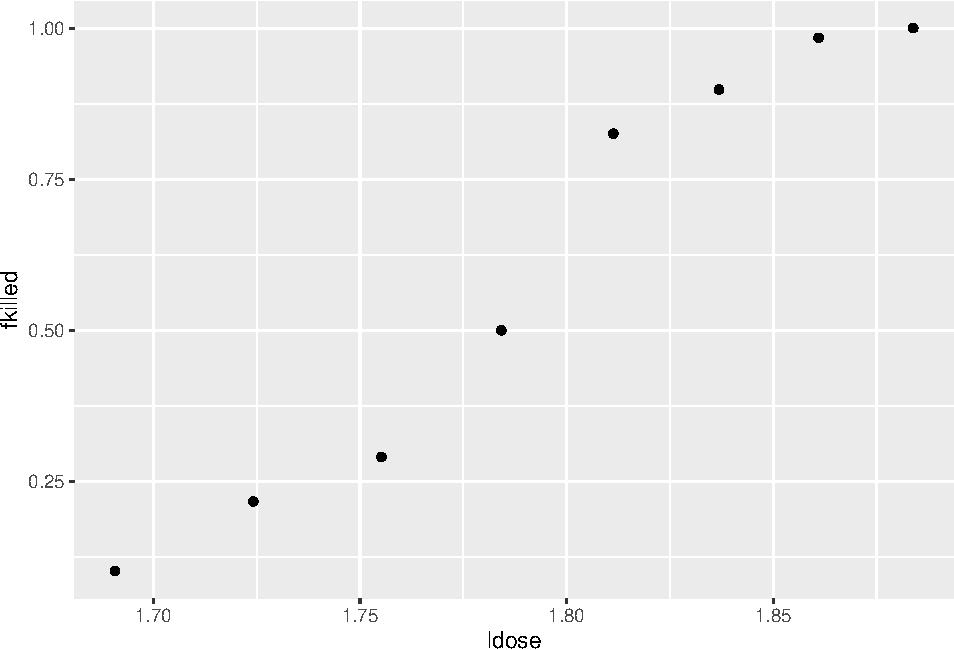
\includegraphics{3BinReg_files/figure-latex/unnamed-chunk-2-1.pdf}

\begin{center}\rule{0.5\linewidth}{0.5pt}\end{center}

\textbf{Q}:

\begin{enumerate}
\def\labelenumi{\alph{enumi}.}
\tightlist
\item
  What might be the effect (mathematical function) of the log10-dose on
  the probability of killing a beetle?
\item
  How can this curve be part of a regression model?
\end{enumerate}

\begin{verbatim}
## Answers
\end{verbatim}

\begin{verbatim}
## a) logistic, sigmoid, normal cdf?.
\end{verbatim}

\begin{verbatim}
## b) see item 3 below - the response function connects the mean of the respons to the linear predictor.
\end{verbatim}

\hypertarget{how-to-model-a-binary-response}{%
\section{How to model a binary
response?}\label{how-to-model-a-binary-response}}

In multiple linear regression we have

\begin{enumerate}
\def\labelenumi{\arabic{enumi}.}
\item
  Random component: Distribution of response:
  \(Y_i\sim N(\mu_i,\sigma^2)\), where \(\mu_i\) is \emph{parameter of
  interest} and \(\sigma^2\) is \emph{nuisance}.
\item
  Systematic component: Linear predictor:
  \(\eta_i={\bf x}_i^T \boldsymbol{\beta}\). Here \({\bf x}_i\) is our
  fixed (not random) \(p\)-dimensional column vector of covariates
  (intercept included).
\item
  Link: Connection between the linear predictor and the mean (parameter
  of interest): \(\mu_i=\eta_i\).
\end{enumerate}

In addition we have independent pairs \(({\bf x}_i,Y_i)\), and assume
that the design matrix - with the covariates for all observation in a
\(n \times p\) matrix - has full rank \(p\).

\begin{itemize}
\tightlist
\item
  It would not make sense to fit the continuous linear regression to
  \(Y_i\) when \(Y_i=\{0,1\}\) - since \(Y_i\) is not a continuous
  random variable, and \(Y_i\) is not normal.
\item
  So, we need to change 1. We keep 2. And, we make 3. more general.
\end{itemize}

\begin{center}\rule{0.5\linewidth}{0.5pt}\end{center}

\hypertarget{idbinary-binary-regression}{%
\subsection{\textless id=``binary''\textgreater{} Binary
regression}\label{idbinary-binary-regression}}

\begin{enumerate}
\def\labelenumi{\arabic{enumi}.}
\tightlist
\item
  \(Y_i \sim \text{bin}(n_i,\pi_i)\). First we study the case that
  \(n_i=1\), that is, each individual observation comes from a Bernoulli
  process with \(n_i=1\) trials (this version of the binomial
  distribution is called the Bernoulli distribution). (Remark: later we
  will also look at ``grouped'' data with \(n_i>1\).) Our parameter of
  interest is \(\pi_i\) which is the mean \(\text{E}(Y_i)=\mu_i=\pi_i\).
\end{enumerate}

\textbf{For a generalized linear model (GLM) we require that the
distribution of the response is an exponential family. We have seen in
M1 that the binomial distribution is an exponential family.}

\begin{center}\rule{0.5\linewidth}{0.5pt}\end{center}

\begin{enumerate}
\def\labelenumi{\arabic{enumi}.}
\setcounter{enumi}{1}
\item
  Linear predictor: \(\eta_i={\bf x}_i^T \boldsymbol{\beta}\).
\item
  We will consider different relationships between the mean
  \(\mu_i=\pi_i\) and the linear predictor \(\eta_i\), and define the
  \emph{link function} \(g\) as \[g(\mu_i)=\eta_i\] and the inverse of
  the link function, called the \emph{response function}, and denoted by
  \[h(\eta_i)=g^{-1}(\eta_i)=\mu_i\]
\end{enumerate}

We thus also have to require that the link function is monotone, and we
will soon see that we also need to require that it is twice
differential.

\textbf{These three ingredients (exponential family distribution of
reponse, linear predictor and choice of reponse or link function) give
the core of our GLM model.}

\begin{center}\rule{0.5\linewidth}{0.5pt}\end{center}

Popular choices for the respons function for binary regression are based
on selecting a cumulative distribution function (cdf) as the response
function. The cdf will always be within {[}0,1{]}, and the cdf is
monotone - which will help us to interpret results.

The most popular response functions are:

\begin{itemize}
\item
  \emph{logistic cdf} (with corresponding \emph{logit} link function)
  referred to as the \emph{logit model}, followed by the
\item
  \emph{normal cdf} - (with corresponding \emph{probit} link function)
  referred to as the \emph{probit model} , and
\item
  the \emph{extreme minimum-value cdf} (with corresponding
  \emph{complementary log-log} link function) referred to as the
  \emph{complementary log-log model}.
\end{itemize}

In this module we focus on the logit model.

\hypertarget{the-logit-model-aka-logistic-regression}{%
\section{The logit model aka logistic
regression}\label{the-logit-model-aka-logistic-regression}}

\hypertarget{beetle-mortality-response-function}{%
\subsection{Beetle mortality: response
function}\label{beetle-mortality-response-function}}

In the beetle example we have a simple linear predictor:
\(\eta_i=\beta_0+\beta_1 x_i\) where \(x_i\) is the log10-dose for
beetle \(i\).

Assume that \(\beta_0=\) -60.7 and \(\beta_1=\) 34.3. (These values are
estimates from our data, and we will see later how to find these
estimates using maximum likelihood estimation.)

Below the response function is plotted for \(\eta_i=\)-60.7+34.3\(x_i\).

\begin{center}\rule{0.5\linewidth}{0.5pt}\end{center}

\begin{Shaded}
\begin{Highlighting}[]
\FunctionTok{library}\NormalTok{(ggplot2)}
\CommentTok{\#print(c(beta0, beta1))}
\NormalTok{xrange}\OtherTok{=}\FunctionTok{range}\NormalTok{(beetleds}\SpecialCharTok{$}\NormalTok{ldose)}
\NormalTok{xrange[}\DecValTok{1}\NormalTok{]}\OtherTok{=}\NormalTok{xrange[}\DecValTok{1}\NormalTok{]}\SpecialCharTok{{-}}\FloatTok{0.05}
\NormalTok{etas}\OtherTok{=}\NormalTok{beta0}\SpecialCharTok{+}\NormalTok{beta1}\SpecialCharTok{*}\FunctionTok{seq}\NormalTok{(xrange[}\DecValTok{1}\NormalTok{],xrange[}\DecValTok{2}\NormalTok{],}\AttributeTok{length=}\DecValTok{100}\NormalTok{)}
\FunctionTok{ggplot}\NormalTok{(}\FunctionTok{data.frame}\NormalTok{(}\AttributeTok{eta=}\FunctionTok{range}\NormalTok{(etas),}\AttributeTok{mu=}\FunctionTok{c}\NormalTok{(}\DecValTok{0}\NormalTok{,}\DecValTok{1}\NormalTok{)), }\FunctionTok{aes}\NormalTok{(eta,mu))}\SpecialCharTok{+}
  \FunctionTok{xlab}\NormalTok{(}\FunctionTok{expression}\NormalTok{(eta))}\SpecialCharTok{+} 
  \FunctionTok{ylab}\NormalTok{(}\FunctionTok{expression}\NormalTok{(mu))}\SpecialCharTok{+}
  \FunctionTok{stat\_function}\NormalTok{(}\AttributeTok{fun=}\ControlFlowTok{function}\NormalTok{(eta) }\FunctionTok{exp}\NormalTok{(eta)}\SpecialCharTok{/}\NormalTok{(}\DecValTok{1}\SpecialCharTok{+}\FunctionTok{exp}\NormalTok{(eta)), }\AttributeTok{geom=}\StringTok{"line"}\NormalTok{, }\AttributeTok{colour=}\StringTok{"red"}\NormalTok{)}
\end{Highlighting}
\end{Shaded}

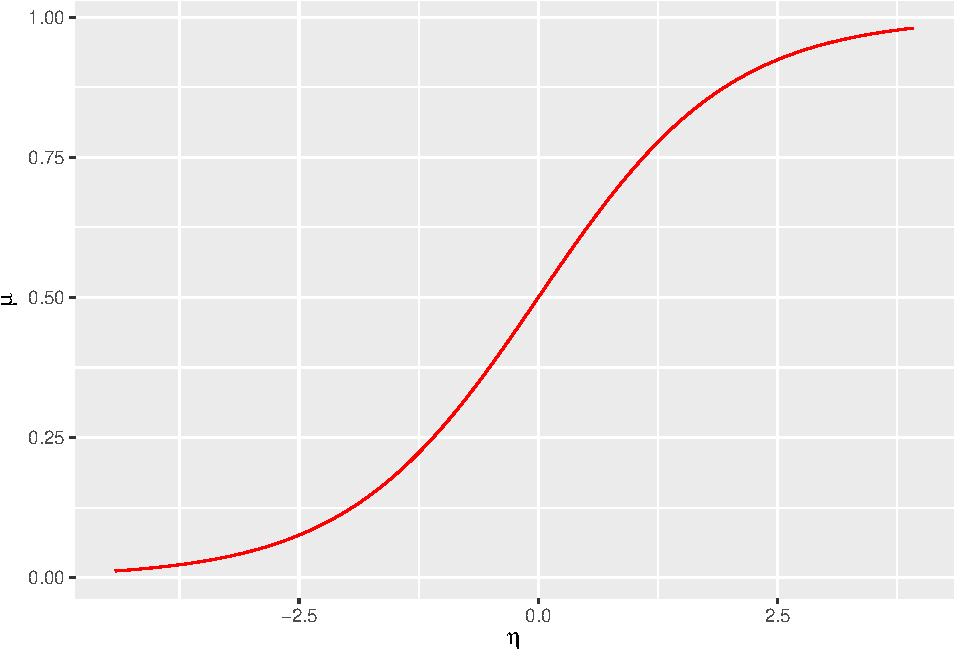
\includegraphics{3BinReg_files/figure-latex/unnamed-chunk-5-1.pdf}

R: more on greek letters with ggplot:
\url{https://github.com/tidyverse/ggplot2/wiki/Plotmath}

\begin{center}\rule{0.5\linewidth}{0.5pt}\end{center}

\textbf{Q}: Explain to your neighbour what is on the x- and y-axis of
this plot. Where are the observed log10-doses in this graph?

\textbf{A}:

On the x-axis is the linear predictor \(\eta=\beta_0+\beta_1 x_1\) for
the given values of \(\beta_0\) and \(\beta_1\) and values for \(x_1\)
is chosen from the range of the log10-dose values. On the y-axis is the
model for the mean of the response, which also here is the probability
of success. This is our non-linear relationship between the linear
predictor and the mean = our response function.

\begin{center}\rule{0.5\linewidth}{0.5pt}\end{center}

\hypertarget{link-and-reponse-function}{%
\subsection{Link and reponse function}\label{link-and-reponse-function}}

The logit model is based on the logistic cdf as the response function,
given as \[ \mu_i=\pi_i=h(\eta_i)=\frac{\exp(\eta_i)}{1+\exp(\eta_i)}\]
or alternatively as the link function (the inverse of the response
function)
\[ g(\mu_i)=h^{-1}(\mu_i)=\ln(\frac{\mu_i}{1-\mu_i})=\ln(\frac{\pi_i}{1-\pi_i})\]

\textbf{Hands-on}: show this for yourself.

\begin{center}\rule{0.5\linewidth}{0.5pt}\end{center}

\hypertarget{interpreting-the-logit-model}{%
\subsection{Interpreting the logit
model}\label{interpreting-the-logit-model}}

If the value of the linear predictor \(\eta_i\) changes to \(\eta_i+1\)
the probability \(\pi\) increases non-linearly from
\(\frac{\exp(\eta_i)}{1+\exp(\eta_i)}\) to
\(\frac{\exp(\eta_i+1)}{1+\exp(\eta_i+1)}\), as shown in the graph
above.

\begin{center}\rule{0.5\linewidth}{0.5pt}\end{center}

Before we go further: do you know about the odds? The ratio
\(\frac{P(Y_i=1)}{P(Y_i=0)}=\frac{\pi_i}{1-\pi_1}\) is called the
\emph{odds}. If \(\pi_i=\frac{1}{2}\) then the odds is \(1\), and if
\(\pi_i=\frac{1}{4}\) then the odds is \(\frac{1}{3}\). We may make a
table for probability vs.~odds in R:

\begin{Shaded}
\begin{Highlighting}[]
\FunctionTok{library}\NormalTok{(knitr)}
\FunctionTok{library}\NormalTok{(kableExtra)}
\NormalTok{pivec}\OtherTok{=}\FunctionTok{seq}\NormalTok{(}\FloatTok{0.1}\NormalTok{,}\FloatTok{0.9}\NormalTok{,}\FloatTok{0.1}\NormalTok{)}
\NormalTok{odds}\OtherTok{=}\NormalTok{pivec}\SpecialCharTok{/}\NormalTok{(}\DecValTok{1}\SpecialCharTok{{-}}\NormalTok{pivec)}
\FunctionTok{kable}\NormalTok{(}\FunctionTok{t}\NormalTok{(}\FunctionTok{data.frame}\NormalTok{(pivec,odds)),}\AttributeTok{digits=}\FunctionTok{c}\NormalTok{(}\DecValTok{2}\NormalTok{,}\DecValTok{2}\NormalTok{))}\SpecialCharTok{\%\textgreater{}\%}
  \FunctionTok{kable\_styling}\NormalTok{()}
\end{Highlighting}
\end{Shaded}

\begin{table}
\centering
\begin{tabular}{l|r|r|r|r|r|r|r|r|r}
\hline
pivec & 0.10 & 0.20 & 0.30 & 0.40 & 0.5 & 0.6 & 0.70 & 0.8 & 0.9\\
\hline
odds & 0.11 & 0.25 & 0.43 & 0.67 & 1.0 & 1.5 & 2.33 & 4.0 & 9.0\\
\hline
\end{tabular}
\end{table}

\begin{center}\rule{0.5\linewidth}{0.5pt}\end{center}

\begin{Shaded}
\begin{Highlighting}[]
\FunctionTok{library}\NormalTok{(knitr)}
\FunctionTok{library}\NormalTok{(kableExtra)}
\NormalTok{pivec}\OtherTok{=}\FunctionTok{seq}\NormalTok{(}\FloatTok{0.1}\NormalTok{,}\FloatTok{0.9}\NormalTok{,}\FloatTok{0.1}\NormalTok{)}
\NormalTok{odds}\OtherTok{=}\NormalTok{pivec}\SpecialCharTok{/}\NormalTok{(}\DecValTok{1}\SpecialCharTok{{-}}\NormalTok{pivec)}
\FunctionTok{plot}\NormalTok{(pivec,odds,}\AttributeTok{type=}\StringTok{"b"}\NormalTok{,}\AttributeTok{ylab=}\StringTok{"odds"}\NormalTok{,}\AttributeTok{xlab=}\StringTok{"probability"}\NormalTok{)}
\end{Highlighting}
\end{Shaded}

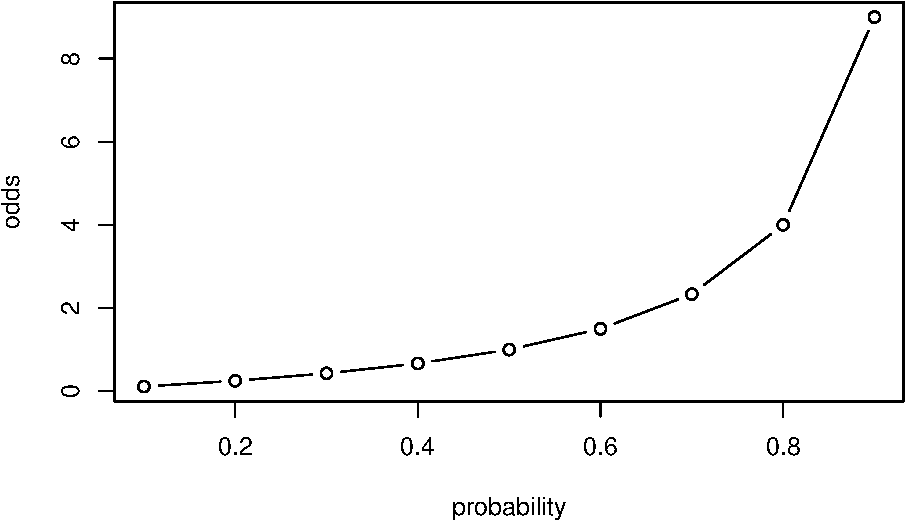
\includegraphics{3BinReg_files/figure-latex/unnamed-chunk-8-1.pdf}

R: Pretty table with
\href{https://cran.r-project.org/web/packages/kableExtra/vignettes/awesome_table_in_html.html}{kableExtra}

Odds may be seen to be a better scale than probability to represent
chance, and is used in betting. In addition, odds are unbounded above.

\begin{center}\rule{0.5\linewidth}{0.5pt}\end{center}

We look at the link function (inverse of the response function). Let us
assume that our linear predictor has \(k\) covariates present

\begin{align*}
\eta_i&= \beta_0+\beta_1 x_{i1}+\beta_2 x_{i2}+\cdots + \beta_k x_{ik}\\
\pi_i&= \frac{\exp(\eta_i)}{1+\exp(\eta_i)}\\
\eta_i&=\ln(\frac{\pi_i}{1-\pi_i})\\
\ln(\frac{\pi_i}{1-\pi_i})&=\beta_0+\beta_1 x_{i1}+\beta_2 x_{i2}+\cdots + \beta_k x_{ik}\\
\frac{\pi_i}{1-\pi_i}=&\frac{P(Y_i=1)}{P(Y_i=0)}=\exp(\beta_0)\cdot \exp(\beta_1 x_{i1})\cdots\exp(\beta_k x_{ik})
\end{align*}

We have a \emph{multiplicative model} for the odds.

\begin{center}\rule{0.5\linewidth}{0.5pt}\end{center}

\textbf{So, what if we increase \(x_{1i}\) to \(x_{1i}+1\)?}

If the covariate \(x_{1i}\) increases by one unit (while all other
covariates are kept fixed) then the odds is multiplied by
\(\exp(\beta_1)\):

\begin{align*}
\frac{P(Y_i=1\mid x_{i1}+1)}{P(Y_i=0)\mid x_{i1}+1)}&=\exp(\beta_0)\cdot \exp(\beta_1 (x_{i1}+1))\cdots\exp(\beta_k x_{ik})\\
&=\exp(\beta_0)\cdot \exp(\beta_1 x_{i1})\exp(\beta_1)\cdots\exp(\beta_k x_{ik})\\
&=\frac{P(Y_i=1\mid x_{i1})}{P(Y_i=0\mid x_{i1})}\cdot \exp(\beta_1)\\
\end{align*}

This means that if \(x_{i1}\) increases by \(1\) then: if \(\beta_1<0\)
we get a decrease in the odds, if \(\beta_1=0\) no change, and if
\(\beta_1>0\) we have an increase. In the logit model \(\exp(\beta_1)\)
is easier to interpret than \(\beta_1\).

\begin{center}\rule{0.5\linewidth}{0.5pt}\end{center}

\textbf{So, to sum up: for the linear predictor we interpret effects in
the same way as for the linear model (in Module 2), then we transform
this linear effect in \(\eta\) into a nonlinear effect for
\(\pi=\frac{\exp(\eta)}{1+\exp(\eta)}\), and use the odds to interpret
changes.}

\begin{center}\rule{0.5\linewidth}{0.5pt}\end{center}

\#\#Infant respitory disease : interpretation of parameter estimates
(This example is taken from Faraway (2006): ``Extending the linar model
with R'')

We select a sample of newborn babies (girls and boys) where the parents
had decided on the method of feeding (bottle, breast, breast with some
supplement), and then monitored the babies during their first year to
see if they developed infant respiratory disease (the event we want to
model).

We fit a logistic regression to the data, and focus on the parameter
estimates.

\begin{center}\rule{0.5\linewidth}{0.5pt}\end{center}

\begin{Shaded}
\begin{Highlighting}[]
\FunctionTok{library}\NormalTok{(faraway)}
\FunctionTok{data}\NormalTok{(babyfood)}
\NormalTok{babyfood}
\end{Highlighting}
\end{Shaded}

\begin{verbatim}
##   disease nondisease  sex   food
## 1      77        381  Boy Bottle
## 2      19        128  Boy  Suppl
## 3      47        447  Boy Breast
## 4      48        336 Girl Bottle
## 5      16        111 Girl  Suppl
## 6      31        433 Girl Breast
\end{verbatim}

\begin{Shaded}
\begin{Highlighting}[]
\FunctionTok{xtabs}\NormalTok{(disease}\SpecialCharTok{/}\NormalTok{(disease}\SpecialCharTok{+}\NormalTok{nondisease)}\SpecialCharTok{\textasciitilde{}}\NormalTok{sex}\SpecialCharTok{+}\NormalTok{food,babyfood)}
\end{Highlighting}
\end{Shaded}

\begin{verbatim}
##       food
## sex        Bottle     Breast      Suppl
##   Boy  0.16812227 0.09514170 0.12925170
##   Girl 0.12500000 0.06681034 0.12598425
\end{verbatim}

\begin{center}\rule{0.5\linewidth}{0.5pt}\end{center}

\footnotesize

\begin{Shaded}
\begin{Highlighting}[]
\NormalTok{fit}\OtherTok{=}\FunctionTok{glm}\NormalTok{(}\FunctionTok{cbind}\NormalTok{(disease, nondisease)}\SpecialCharTok{\textasciitilde{}}\NormalTok{sex}\SpecialCharTok{+}\NormalTok{food,}\AttributeTok{family=}\FunctionTok{binomial}\NormalTok{(}\AttributeTok{link=}\NormalTok{logit),}\AttributeTok{data=}\NormalTok{babyfood)}
\FunctionTok{summary}\NormalTok{(fit)}
\end{Highlighting}
\end{Shaded}

\begin{verbatim}
## 
## Call:
## glm(formula = cbind(disease, nondisease) ~ sex + food, family = binomial(link = logit), 
##     data = babyfood)
## 
## Coefficients:
##             Estimate Std. Error z value Pr(>|z|)    
## (Intercept)  -1.6127     0.1124 -14.347  < 2e-16 ***
## sexGirl      -0.3126     0.1410  -2.216   0.0267 *  
## foodBreast   -0.6693     0.1530  -4.374 1.22e-05 ***
## foodSuppl    -0.1725     0.2056  -0.839   0.4013    
## ---
## Signif. codes:  0 '***' 0.001 '**' 0.01 '*' 0.05 '.' 0.1 ' ' 1
## 
## (Dispersion parameter for binomial family taken to be 1)
## 
##     Null deviance: 26.37529  on 5  degrees of freedom
## Residual deviance:  0.72192  on 2  degrees of freedom
## AIC: 40.24
## 
## Number of Fisher Scoring iterations: 4
\end{verbatim}

\begin{Shaded}
\begin{Highlighting}[]
\FunctionTok{exp}\NormalTok{(fit}\SpecialCharTok{$}\NormalTok{coefficients)}
\end{Highlighting}
\end{Shaded}

\begin{verbatim}
## (Intercept)     sexGirl  foodBreast   foodSuppl 
##   0.1993479   0.7315770   0.5120696   0.8415226
\end{verbatim}

\begin{Shaded}
\begin{Highlighting}[]
\FunctionTok{predict}\NormalTok{(fit,}\AttributeTok{type=}\StringTok{"response"}\NormalTok{) }\CommentTok{\#gives predicted probabilites}
\end{Highlighting}
\end{Shaded}

\begin{verbatim}
##          1          2          3          4          5          6 
## 0.16621356 0.14365654 0.09262485 0.12727653 0.10931093 0.06948992
\end{verbatim}

\normalsize

\begin{center}\rule{0.5\linewidth}{0.5pt}\end{center}

\textbf{Q:} Observe that the two factors by default is coded with dummy
variable coding, and that \texttt{sexBoy} is the reference category for
sex and \texttt{foodBottle} the reference category for feeding method.

1: Explain how to interpret the \texttt{Estimate} for \texttt{sexGirl},
\texttt{foodBreast} and \texttt{foodSuppl}.

2: What are the 6 values given by the call to \texttt{predict}? What is
the least favourable combination of sex and method of feeding? And the
most favourable?

Comment: we have here fitted an additive model in the two covariates,
but we could also include an interaction term. This will be discussed
later.

\begin{center}\rule{0.5\linewidth}{0.5pt}\end{center}

\hypertarget{more-response-function-plots-for-the-logit-model}{%
\subsection{More response function plots for the logit
model}\label{more-response-function-plots-for-the-logit-model}}

The response function as a function of the covariate \(x\) and not of
\(\eta\). Solid lines: \(\beta_0=0\) and \(\beta_1\) is \(0.8\) (blue),
\(1\) (red) and \(2\) (orange), and dashed lines with \(\beta_0=1\).

\begin{Shaded}
\begin{Highlighting}[]
\FunctionTok{library}\NormalTok{(ggplot2)}
\FunctionTok{ggplot}\NormalTok{(}\FunctionTok{data.frame}\NormalTok{(}\AttributeTok{x=}\FunctionTok{c}\NormalTok{(}\SpecialCharTok{{-}}\DecValTok{6}\NormalTok{,}\DecValTok{5}\NormalTok{)), }\FunctionTok{aes}\NormalTok{(x))}\SpecialCharTok{+}
  \FunctionTok{xlab}\NormalTok{(}\FunctionTok{expression}\NormalTok{(x))}\SpecialCharTok{+} 
  \FunctionTok{ylab}\NormalTok{(}\FunctionTok{expression}\NormalTok{(mu))}\SpecialCharTok{+}
    \FunctionTok{stat\_function}\NormalTok{(}\AttributeTok{fun=}\ControlFlowTok{function}\NormalTok{(x) }\FunctionTok{exp}\NormalTok{(x)}\SpecialCharTok{/}\NormalTok{(}\DecValTok{1}\SpecialCharTok{+}\FunctionTok{exp}\NormalTok{(x)), }\AttributeTok{geom=}\StringTok{"line"}\NormalTok{, }\AttributeTok{colour=}\StringTok{"red"}\NormalTok{)}\SpecialCharTok{+}
    \FunctionTok{stat\_function}\NormalTok{(}\AttributeTok{fun=}\ControlFlowTok{function}\NormalTok{(x) }\FunctionTok{exp}\NormalTok{(}\DecValTok{2}\SpecialCharTok{*}\NormalTok{x)}\SpecialCharTok{/}\NormalTok{(}\DecValTok{1}\SpecialCharTok{+}\FunctionTok{exp}\NormalTok{(}\DecValTok{2}\SpecialCharTok{*}\NormalTok{x)), }\AttributeTok{geom=}\StringTok{"line"}\NormalTok{, }\AttributeTok{colour=}\StringTok{"orange"}\NormalTok{)}\SpecialCharTok{+}
          \FunctionTok{stat\_function}\NormalTok{(}\AttributeTok{fun=}\ControlFlowTok{function}\NormalTok{(x) }\FunctionTok{exp}\NormalTok{(}\FloatTok{0.8}\SpecialCharTok{*}\NormalTok{x)}\SpecialCharTok{/}\NormalTok{(}\DecValTok{1}\SpecialCharTok{+}\FunctionTok{exp}\NormalTok{(}\FloatTok{0.8}\SpecialCharTok{*}\NormalTok{x)), }\AttributeTok{geom=}\StringTok{"line"}\NormalTok{, }\AttributeTok{colour=}\StringTok{"blue"}\NormalTok{)}\SpecialCharTok{+}
    \FunctionTok{stat\_function}\NormalTok{(}\AttributeTok{fun=}\ControlFlowTok{function}\NormalTok{(x) }\FunctionTok{exp}\NormalTok{(}\DecValTok{1}\SpecialCharTok{+}\NormalTok{x)}\SpecialCharTok{/}\NormalTok{(}\DecValTok{1}\SpecialCharTok{+}\FunctionTok{exp}\NormalTok{(}\DecValTok{1}\SpecialCharTok{+}\NormalTok{x)), }\AttributeTok{geom=}\StringTok{"line"}\NormalTok{, }\AttributeTok{colour=}\StringTok{"red"}\NormalTok{,}\AttributeTok{linetype=}\StringTok{"dashed"}\NormalTok{)}\SpecialCharTok{+}
    \FunctionTok{stat\_function}\NormalTok{(}\AttributeTok{fun=}\ControlFlowTok{function}\NormalTok{(x) }\FunctionTok{exp}\NormalTok{(}\DecValTok{1}\SpecialCharTok{+}\DecValTok{2}\SpecialCharTok{*}\NormalTok{x)}\SpecialCharTok{/}\NormalTok{(}\DecValTok{1}\SpecialCharTok{+}\FunctionTok{exp}\NormalTok{(}\DecValTok{1}\SpecialCharTok{+}\DecValTok{2}\SpecialCharTok{*}\NormalTok{x)), }\AttributeTok{geom=}\StringTok{"line"}\NormalTok{, }\AttributeTok{colour=}\StringTok{"orange"}\NormalTok{,}\AttributeTok{linetype=}\StringTok{"dashed"}\NormalTok{)}\SpecialCharTok{+}
          \FunctionTok{stat\_function}\NormalTok{(}\AttributeTok{fun=}\ControlFlowTok{function}\NormalTok{(x) }\FunctionTok{exp}\NormalTok{(}\DecValTok{1}\FloatTok{+0.8}\SpecialCharTok{*}\NormalTok{x)}\SpecialCharTok{/}\NormalTok{(}\DecValTok{1}\SpecialCharTok{+}\FunctionTok{exp}\NormalTok{(}\DecValTok{1}\FloatTok{+0.8}\SpecialCharTok{*}\NormalTok{x)), }\AttributeTok{geom=}\StringTok{"line"}\NormalTok{, }\AttributeTok{colour=}\StringTok{"blue"}\NormalTok{,}\AttributeTok{linetype=}\StringTok{"dashed"}\NormalTok{)}\SpecialCharTok{+}
  \FunctionTok{scale\_colour\_manual}\NormalTok{(}\StringTok{"0+k x"}\NormalTok{,}\AttributeTok{values =} \FunctionTok{c}\NormalTok{(}\StringTok{"red"}\NormalTok{, }\StringTok{"orange"}\NormalTok{,}\StringTok{"blue"}\NormalTok{),}\AttributeTok{labels=}\FunctionTok{c}\NormalTok{(}\StringTok{"1"}\NormalTok{,}\StringTok{"2"}\NormalTok{,}\StringTok{"0.8"}\NormalTok{))}
\end{Highlighting}
\end{Shaded}

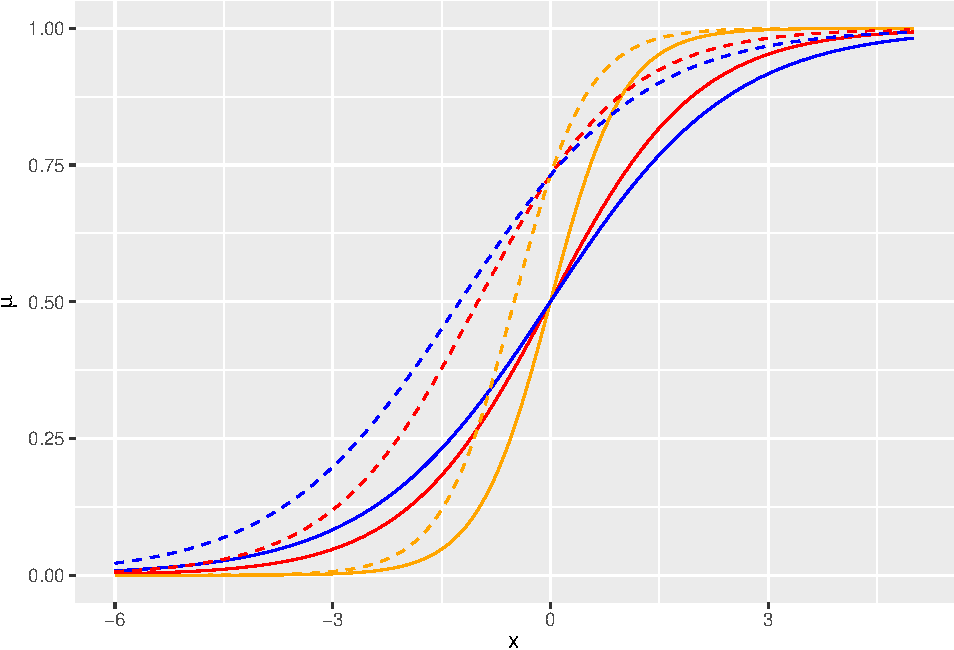
\includegraphics{3BinReg_files/figure-latex/unnamed-chunk-12-1.pdf}

\hypertarget{grouped-vs.-individual-data}{%
\section{Grouped vs.~individual
data}\label{grouped-vs.-individual-data}}

So far we have only mentioned individual (ungrouped) data. That is,
every \(Y_i\) is 0 or 1 and has a corresponding covariate vector
\({\bf x}_i\) - and together they form \emph{one} unit.
\[Y_i \sim \text{bin}(n_i=1,\pi_i)\] However, in both the examples we
have looked at some covariate vectors are \emph{identical} (rows in the
design matrix are identical). We call these unique combinations of
covariates \emph{covariate patterns}, and say we have \emph{grouped}
data.

\begin{Shaded}
\begin{Highlighting}[]
\FunctionTok{library}\NormalTok{(kableExtra)}
\NormalTok{knitr}\SpecialCharTok{::}\FunctionTok{kable}\NormalTok{(babyfood) }\SpecialCharTok{\%\textgreater{}\%}
  \FunctionTok{kable\_styling}\NormalTok{(}\AttributeTok{bootstrap\_options =} \FunctionTok{c}\NormalTok{(}\StringTok{"striped"}\NormalTok{, }\StringTok{"hover"}\NormalTok{))}
\end{Highlighting}
\end{Shaded}

\begin{table}
\centering
\begin{tabular}{r|r|l|l}
\hline
disease & nondisease & sex & food\\
\hline
77 & 381 & Boy & Bottle\\
\hline
19 & 128 & Boy & Suppl\\
\hline
47 & 447 & Boy & Breast\\
\hline
48 & 336 & Girl & Bottle\\
\hline
16 & 111 & Girl & Suppl\\
\hline
31 & 433 & Girl & Breast\\
\hline
\end{tabular}
\end{table}

\begin{center}\rule{0.5\linewidth}{0.5pt}\end{center}

Here we have 6 groups of covariate patterns. The first group has
covariates \texttt{Boy} and \texttt{Bottle}, there are 77+381= 458
babies with this combination and 77 of these got the disease.

We prefer to group data if possible. Grouping is good because then data
can be kept in a condenced form, it will speed up computations and makes
model diagnosis easier (than for individual data).

\begin{center}\rule{0.5\linewidth}{0.5pt}\end{center}

For the grouped data we still have a binomial distribution, and possible
generalization is to let

\begin{itemize}
\tightlist
\item
  \(n_j\bar{Y_j}\) be the number of successes in group \(j\),
\item
  which means that \(\bar{Y_j}=\frac{1}{n_j}\sum Y_i\) where the sum is
  over all \(i\) in group \(j\).
\end{itemize}

Further \[ n_j\bar{Y_j} \sim \text{bin}(n_j,\pi_j)\] such that
\(\text{E}(n_j\bar{Y_j})=n_j \pi_j\) and
\(\text{Var}(n_j\bar{Y_j})=n_j \pi_j(1-\pi_j)\), and
\(\text{E}(\bar{Y_j})=\pi_j\) and
\(\text{Var}(\bar{Y_j})=\frac{1}{n_j} \pi_j(1-\pi_j)\)

We then keep the linear predictor, and the link function is still
\(\eta_j=\ln(\frac{\pi_j}{1-\pi_j})\). That is, we do not model the mean
\(n_j \pi_j\) but \(\pi_j\) directly.

\textbf{Q:} What is a covariate pattern?

\begin{verbatim}
## Answer
\end{verbatim}

\begin{verbatim}
## A set of values for covariates that are the same for a group of individual data. For the beetle example we have 8 covariate patterns - the 8 dosages, while for the infant respiratory disease we have 6 covariate patterns (boy, girl)*(bottle, supplement, breast). So, unique rows of the design matrix.
\end{verbatim}

\hypertarget{likelihood-and-derivations-thereof}{%
\section{Likelihood and derivations
thereof}\label{likelihood-and-derivations-thereof}}

Our parameter of interest is the vector \(\boldsymbol{\beta}\) of
regression coefficients, and we have no nuicance parameters (because the
variance is related directly to the \(\pi_j\) and \(n_j\) is known).

We would like to estimate \(\boldsymbol{\beta}\) from maximizing the
likelihood, but we will soon see that we have no closed form solution.
First we look at the likelihood, the log-likelihood and first and second
derivatives thereof.

For simplicity we do the derivations for the case where \(n_i=1\), but
then include the results for the case where we have \(G\) covariate
patterns with \(n_j\) observations of each pattern.

\begin{center}\rule{0.5\linewidth}{0.5pt}\end{center}

\textbf{Assumptions:}

\begin{enumerate}
\def\labelenumi{\arabic{enumi}.}
\item
  \(Y_i \sim \text{bin}(n_i=1,\pi_i)\), and
  \(\text{E}(Y_i)=\mu_i=\pi_i\), and \(\text{Var}(Y_i)=\pi_i(1-\pi_i)\).
\item
  Linear predictor: \(\eta_i={\bf x}_i^T \boldsymbol{\beta}\).
\item
  Logit link \[\eta_i=\ln(\frac{\pi_i}{1-\pi_i})=g(\mu_i)\] and (inverse
  thereof) logistic response function
  \[\mu_i=\pi_i=\frac{\exp(\eta_i)}{1+\exp(\eta_i)}=h(\eta_i)\]
\end{enumerate}

We will also need:
\[(1-\pi_i)=1-\frac{\exp(\eta_i)}{1+\exp(\eta_i)}=\frac{1+\exp(\eta_i)-\exp(\eta_i)}{1+\exp(\eta_i)}=\frac{1}{1+\exp(\eta_i)}.\]

\begin{center}\rule{0.5\linewidth}{0.5pt}\end{center}

\hypertarget{likelihood-lboldsymbolbeta}{%
\subsection{\texorpdfstring{Likelihood
\(L(\boldsymbol{\beta})\)}{Likelihood L(\textbackslash boldsymbol\{\textbackslash beta\})}}\label{likelihood-lboldsymbolbeta}}

We assume that pairs of covariates and response are measured
independently of each other: \(({\bf x}_i,Y_i)\), and \(Y_i\) follows
the distribution specified above, and \({\bf x}_i\) is fixed.

\[L(\boldsymbol{\beta})=\prod_{i=1}^n L_i(\boldsymbol{\beta})=\prod_{i=1}^n f(y_i; \boldsymbol{\beta})=\prod_{i=1}^n\pi_i^{y_i}(1-\pi_i)^{1-y_i}\]

\textbf{Q}: What is the interpretation of the likelihood? Is it not a
misuse of notation to write \(L(\boldsymbol{\beta})\) when the right
hand side does not involve \(\boldsymbol{\beta}\)?

\textbf{A}:

The likelihood is the joint distribution of the responses, but with
focus on the unknown parameter vector. Yes, a slight misuse of notation,
need to fill in \(\pi_i=h(\eta_i)\) and
\(\eta_i={\bf x}^T\boldsymbol{\beta}\) to write out
\(L(\boldsymbol{\beta})\), really. But we keep this version because when
we want to take the partical derivatives we will use the chain rule.

\begin{center}\rule{0.5\linewidth}{0.5pt}\end{center}

\hypertarget{loglikelihood-lboldsymbolbeta}{%
\subsection{\texorpdfstring{Loglikelihood
\(l(\boldsymbol{\beta})\)}{Loglikelihood l(\textbackslash boldsymbol\{\textbackslash beta\})}}\label{loglikelihood-lboldsymbolbeta}}

The log-likelihood is the natural log of the likelihood, and makes the
mathematics simpler - since we work with exponential families. The main
aim with the likelihood is to maximize it to find the maximum likelihood
estimate, and since the log is a monotone function the maximum of the
log-likelihood will be in the same place as the maximum of the
likelihood.

\begin{align}
l(\boldsymbol{\beta})&=\ln L(\boldsymbol{\beta})=\sum_{i=1}^n \ln L_i(\boldsymbol{\beta})=\sum_{i=1}^n l_i(\boldsymbol{\beta})\\
&=\sum_{i=1}^n[y_i \ln \pi_i+(1-y_i) \ln(1-\pi_i)]\\
&=\sum_{i=1}^n[y_i \ln (\frac{\pi_i}{1-\pi_i})+\ln(1-\pi_i)]
\end{align}

Observe that the log-likelihood is a sum of invidual contributions for
each observation pair \(i\).

\begin{center}\rule{0.5\linewidth}{0.5pt}\end{center}

The log-likelihood is now expressed as a function of \(\pi_i\), but we
want to make this a function of \(\boldsymbol{\beta}\) and the
connection between \(\pi_i\) and \(\boldsymbol{\beta}\) goes through
\(\eta_i\). We have that \(\pi=\frac{\exp(\eta_i)}{1+\exp(\eta_i)}\) and
in our log-likelihood we need

\[(1-\pi_i)=\frac{1}{1+\exp(\eta_i)}=\frac{1+\exp(\eta_i)-\exp(\eta_i)}{1+\exp(\eta_i)}=\frac{1}{1+\exp(\eta_i)}\]
and \[\ln(\frac{\pi_i}{1-\pi_1})=\eta_i\] (the last is our logit link
function). Then we get:

\[l(\boldsymbol{\beta})=\sum_{i=1}^n[y_i \eta_i + \ln (\frac{1}{1+\exp(\eta_i)})]=\sum_{i=1}^n[y_i \eta_i - \ln (1+\exp(\eta_i))]\]
which is now our function of \(\eta_i\).

\begin{center}\rule{0.5\linewidth}{0.5pt}\end{center}

Finally, since \(\eta_i={\bf x}_i^T \boldsymbol{\beta}\),
\[l(\boldsymbol{\beta})=\sum_{i=1}^n[y_i {\bf x}_i^T \boldsymbol{\beta} - \ln (1+\exp({\bf x}_i^T \boldsymbol{\beta}))].\]

\textbf{Q}: What does the graph of \(l\) look like as a function of
\(\boldsymbol{\beta}\)?

If we look at the beetle example we only have one covariate (in addition
to the intercept) - so this means that we have
\(\boldsymbol{\beta}=(\beta_0,\beta_1)\). Plotting the log-likelihood
(for the beetle data set) will be one of the tasks for the interactive
lecture.

\textbf{But, next we take partial derivatives, and then we will (instead
of using this formula) look at
\(l_i(\boldsymbol{\beta})=l_i(\eta_i(\boldsymbol{\beta}))\) and use the
chain rule.}

\begin{center}\rule{0.5\linewidth}{0.5pt}\end{center}

\hypertarget{score-function-sboldsymbolbeta}{%
\subsection{\texorpdfstring{Score function
\(s(\boldsymbol{\beta})\)}{Score function s(\textbackslash boldsymbol\{\textbackslash beta\})}}\label{score-function-sboldsymbolbeta}}

The score function is a \(p\times 1\) vector, \(s(\boldsymbol{\beta})\),
with the partial derivatives of the log-likelihood with respect to the
\(p\) elements of the \(\boldsymbol{\beta}\) vector.

\textbf{Q}: Write down the rules for derivatives: chain rule, product
rule, fraction rule, and in particular derivative of \(\ln(x)\),
\(\exp(x)\) and \(\frac{1}{x}\), you will need them now.

\textbf{A:} Chain rule:
\(\frac{d f(u(x))}{du}=\frac{df}{du}\cdot \frac{du}{dx}\), product rule:
\((u\cdot v)'=u'\cdot v+u\cdot v'\), fraction rule:
\((\frac{u}{v})'=\frac{u' \cdot v - u\cdot v'}{v^2}\),
\(\frac{d \ln(x)}{dx}=\frac{1}{x}\), \(\frac{d\exp(x)}{dx}=\exp(x)\) and
\(\frac{d(\frac{1}{x})}{dx}=-\frac{1}{x^2}\).

Here we go:
\[s(\boldsymbol{\beta})=\frac{\partial l(\boldsymbol{\beta})}{\partial \boldsymbol{\beta}}=
\sum_{i=1}^n \frac{\partial l_i(\boldsymbol{\beta})}{\partial \boldsymbol{\beta}}=
\sum_{i=1}^n s_i(\boldsymbol{\beta})\]

Again, observe that the score function is a sum of individual
contributions for each observation pair \(i\).

\begin{center}\rule{0.5\linewidth}{0.5pt}\end{center}

We will use the chain rule to calculate \(s_i(\boldsymbol{\beta})\).

\[s_i(\boldsymbol{\beta})=\frac{\partial l_i(\boldsymbol{\beta})}{\partial \boldsymbol{\beta}}=\frac{\partial l_i(\boldsymbol{\beta})}{\partial \eta_i}\cdot \frac{\partial \eta_i}{\partial \boldsymbol{\beta}}=\frac{\partial [y_i\eta_i-\ln(1+{\exp(\eta_i)})]}{\partial \eta_i}\cdot \frac{\partial [{\bf x}_i^T\boldsymbol{\beta} ]}{\partial \boldsymbol{\beta}}\]

\[s_i(\boldsymbol{\beta})=(y_i-\frac{\exp(\eta_i)}{1+\exp(\eta_i)})\cdot {\bf x}_i=(y_i-\pi_i) {\bf x}_i \]

\begin{center}\rule{0.5\linewidth}{0.5pt}\end{center}

Here we have used the general rule for all partial derivatives of scalar
with respect to vector (also used in TMA4267):
\[\frac{\partial{\bf a}^T{\bf b}}{\partial {\bf b}}={\bf a}\] and later
we will also need
\[\frac{\partial{\bf a}^T{\bf b}}{\partial {\bf b}^T}=(\frac{\partial{\bf a}^T{\bf b}}{\partial {\bf b}})^T={\bf a}^T.\]

\begin{center}\rule{0.5\linewidth}{0.5pt}\end{center}

The score function is given as:

\[s(\boldsymbol{\beta})=\sum_{i=1}^n s_i(\boldsymbol{\beta})=\sum_{i=1}^n {\bf x}_i (y_i-\pi_i)=\sum_{i=1}^n {\bf x}_i (y_i-\frac{\exp({\bf x}_i^T\boldsymbol{\beta})}{1+\exp({\bf x}_i^T\boldsymbol{\beta})})\]

To find the maximum likelihood estimate \(\hat{\boldsymbol{\beta}}\) we
solve the set of \(p\) non-linear equations:
\[s(\hat{\boldsymbol{\beta}})=0\]

We will soon see how we can do that using the Newton-Raphson or Fisher
Scoring iterative methods, but first we will work on finding the mean
and covariance matrix of the score vector - and the derivatives of the
score vector (the Hessian, which is minus the observed Fisher matrix).

\begin{center}\rule{0.5\linewidth}{0.5pt}\end{center}

\textbf{Remark}: in Module 5 we will see that the general formula for
GLMs is: \[s(\boldsymbol{\beta})=\sum_{i=1}^n
[\frac{y_i-\mu_i}{\text{Var}(Y_i)}{\bf x}_i \frac{\partial \mu_i}{\partial \eta_i}]=\sum_{i=1}^n
[\frac{y_i-\mu_i}{\text{Var}(Y_i)}{\bf x}_i h'(\eta_i)]={\bf X}^T {\bf D} \Sigma^{-1} ({\bf y} -\mu)\]
where \({\bf X}\) is the \(n\times p\) design matrix,
\({\bf D}=\text{diag}(h'(\eta_1),h'(\eta_2),\ldots,h'(\eta_n))\) is a
diagonal matrix with the derivatives of the response function evaluated
at each observation. Further,
\(\Sigma=\text{diag}(\text{Var}(Y_1),\text{Var}(Y_2),\ldots,\text{Var}(Y_n))\)
is a diagonal matrix with the variance for each response, and
\({\bf y}\) is the observed \(n\times 1\) vector of responses and
\(\mu\) is the \(n\times 1\) vector of individual expectations
\(\mu_i=\text{E}(Y_i)=h(\eta_i)\).

More in Module 5.

\hypertarget{interactive-lecture---first-week}{%
\section{Interactive lecture - first
week}\label{interactive-lecture---first-week}}

\hypertarget{theoretical-questions---with-and-without-use-of-r}{%
\subsection{Theoretical questions - with and without use of
R}\label{theoretical-questions---with-and-without-use-of-r}}

\hypertarget{problem-1-model-assumptions}{%
\subsubsection{Problem 1: Model
assumptions}\label{problem-1-model-assumptions}}

\begin{enumerate}
\def\labelenumi{\alph{enumi})}
\tightlist
\item
  What are the model assumptions for a binary regression?
\item
  Which link function and response function is used for the logit model?
\item
  What is the difference between the logit model and a logistic
  regression?
\end{enumerate}

\begin{center}\rule{0.5\linewidth}{0.5pt}\end{center}

\hypertarget{problem-2-log-likelihood.}{%
\subsubsection{Problem 2:
Log-likelihood.}\label{problem-2-log-likelihood.}}

\begin{enumerate}
\def\labelenumi{\alph{enumi})}
\item
  What is the definition of the log-likelihood?
\item
  For the logit model the log-likelihood is
  \[l(\boldsymbol{\beta})=\sum_{j=1}^G[\ln \binom{n_j}{y_j}+ y_j \ln \pi_j-y_j\ln(1-\pi_j)+n_j\ln(1-\pi_j)]\]
  for grouped data. Explain how we have arrived at this formula?
\item
  Write the version of the loglikelihood for individual data
  (i.e.~\(n_j=1\) and \(G=n\)).
\item
  Where is \(\boldsymbol{\beta}\) in the loglikelihood in c? Rewrite
  this to be a function of \(\boldsymbol{\beta}\).
\item
  Why can we ignore the normalizing constant (what is the constant?) in
  the case of \(n_j = 1 \ \forall j\)? Considering what the
  log-likelihood is used for, why can we ignore the normalizing constant
  in all cases (i.e., also when \(n_j \neq 1\))?
\item
  What does this graph of \(l\) look like as a function of
  \(\boldsymbol{\beta}\) for the beetle data? First discuss shortly and
  then to aid you in answering this we look at the loglikelihood for the
  beetle data. Read the R code, discuss what is done and work on
  interpreting the final graph - in particular comment on the yellow
  ridge in the plot.
\end{enumerate}

The beetle data has only one covariate (in addition to the intercept) -
so this means that we have
\(\boldsymbol{\beta}=(\boldsymbol{\beta}_0,\boldsymbol{\beta}_1)\). Look
at the following code and explain what is done - remark: we have used
the \(n_i=1\) version of the loglikelihood here.

\begin{Shaded}
\begin{Highlighting}[]
\FunctionTok{library}\NormalTok{(investr)}
\FunctionTok{library}\NormalTok{(ggplot2)}
\FunctionTok{library}\NormalTok{(viridis)}

\CommentTok{\# from aggregated to individual data (because these data were aggregated)}
\NormalTok{ldose }\OtherTok{\textless{}{-}} \FunctionTok{rep}\NormalTok{(investr}\SpecialCharTok{::}\NormalTok{beetle}\SpecialCharTok{$}\NormalTok{ldose, investr}\SpecialCharTok{::}\NormalTok{beetle}\SpecialCharTok{$}\NormalTok{n)}
\NormalTok{y }\OtherTok{\textless{}{-}} \ConstantTok{NULL}
\ControlFlowTok{for}\NormalTok{ (i }\ControlFlowTok{in} \DecValTok{1}\SpecialCharTok{:}\DecValTok{8}\NormalTok{) y }\OtherTok{=} \FunctionTok{c}\NormalTok{(y, }\FunctionTok{rep}\NormalTok{(}\DecValTok{0}\NormalTok{, investr}\SpecialCharTok{::}\NormalTok{beetle}\SpecialCharTok{$}\NormalTok{n[i] }\SpecialCharTok{{-}}\NormalTok{ investr}\SpecialCharTok{::}\NormalTok{beetle}\SpecialCharTok{$}\NormalTok{y[i]), }\FunctionTok{rep}\NormalTok{(}\DecValTok{1}\NormalTok{, investr}\SpecialCharTok{::}\NormalTok{beetle}\SpecialCharTok{$}\NormalTok{y[i]))}
\NormalTok{beetleds }\OtherTok{=} \FunctionTok{data.frame}\NormalTok{(}\AttributeTok{killed =}\NormalTok{ y, }\AttributeTok{ldose =}\NormalTok{ ldose)}

\NormalTok{loglik }\OtherTok{\textless{}{-}} \ControlFlowTok{function}\NormalTok{(par, args)\{}
\NormalTok{  y }\OtherTok{\textless{}{-}}\NormalTok{ args}\SpecialCharTok{$}\NormalTok{y; x }\OtherTok{\textless{}{-}}\NormalTok{ args}\SpecialCharTok{$}\NormalTok{x; n }\OtherTok{\textless{}{-}}\NormalTok{ args}\SpecialCharTok{$}\NormalTok{n}
\NormalTok{  res }\OtherTok{\textless{}{-}} \FunctionTok{sum}\NormalTok{(y}\SpecialCharTok{*}\NormalTok{x}\SpecialCharTok{\%*\%}\NormalTok{par }\SpecialCharTok{{-}}\NormalTok{ n}\SpecialCharTok{*}\FunctionTok{log}\NormalTok{(}\DecValTok{1} \SpecialCharTok{+} \FunctionTok{exp}\NormalTok{(x}\SpecialCharTok{\%*\%}\NormalTok{par)))}
  \FunctionTok{return}\NormalTok{(res)}
\NormalTok{\}}

\FunctionTok{loglik}\NormalTok{(}\FunctionTok{c}\NormalTok{(}\DecValTok{1}\NormalTok{,}\DecValTok{1}\NormalTok{), }\AttributeTok{args =} \FunctionTok{list}\NormalTok{(}\AttributeTok{y =}\NormalTok{ beetleds}\SpecialCharTok{$}\NormalTok{killed, }
                           \AttributeTok{x =} \FunctionTok{cbind}\NormalTok{(}\FunctionTok{rep}\NormalTok{(}\DecValTok{1}\NormalTok{, }\FunctionTok{nrow}\NormalTok{(beetleds)), beetleds}\SpecialCharTok{$}\NormalTok{ldose), }
                           \AttributeTok{n =} \FunctionTok{rep}\NormalTok{(}\DecValTok{1}\NormalTok{, }\FunctionTok{nrow}\NormalTok{(beetleds))))}
\end{Highlighting}
\end{Shaded}

\begin{verbatim}
## [1] -549.2543
\end{verbatim}

\begin{Shaded}
\begin{Highlighting}[]
\NormalTok{loglikmat }\OtherTok{\textless{}{-}} \FunctionTok{matrix}\NormalTok{(}\ConstantTok{NA}\NormalTok{, }\AttributeTok{nrow =} \DecValTok{100}\NormalTok{, }\AttributeTok{ncol =} \DecValTok{100}\NormalTok{)}
\NormalTok{loglikframe }\OtherTok{\textless{}{-}} \FunctionTok{data.frame}\NormalTok{()}
\NormalTok{beta\_0 }\OtherTok{\textless{}{-}} \FunctionTok{seq}\NormalTok{(}\SpecialCharTok{{-}}\DecValTok{90}\NormalTok{,}\SpecialCharTok{{-}}\DecValTok{30}\NormalTok{, }\AttributeTok{length.out =} \DecValTok{100}\NormalTok{)}
\NormalTok{beta\_1 }\OtherTok{\textless{}{-}} \FunctionTok{seq}\NormalTok{(}\DecValTok{20}\NormalTok{, }\DecValTok{50}\NormalTok{, }\AttributeTok{length.out =} \DecValTok{100}\NormalTok{)}

\ControlFlowTok{for}\NormalTok{ (i }\ControlFlowTok{in} \DecValTok{1}\SpecialCharTok{:}\FunctionTok{length}\NormalTok{(beta\_0))\{}
  \ControlFlowTok{for}\NormalTok{ (j }\ControlFlowTok{in} \DecValTok{1}\SpecialCharTok{:}\FunctionTok{length}\NormalTok{(beta\_1))\{}
    
\NormalTok{    loglikmat[i,j] }\OtherTok{\textless{}{-}} \FunctionTok{loglik}\NormalTok{(}\FunctionTok{c}\NormalTok{(beta\_0[i], beta\_1[j]), }\AttributeTok{args =} \FunctionTok{list}\NormalTok{(}\AttributeTok{y =}\NormalTok{ beetleds}\SpecialCharTok{$}\NormalTok{killed, }
                                                                  \AttributeTok{x =} \FunctionTok{cbind}\NormalTok{(}\FunctionTok{rep}\NormalTok{(}\DecValTok{1}\NormalTok{, }\FunctionTok{nrow}\NormalTok{(beetleds)), beetleds}\SpecialCharTok{$}\NormalTok{ldose), }
                                                                  \AttributeTok{n =} \FunctionTok{rep}\NormalTok{(}\DecValTok{1}\NormalTok{, }\FunctionTok{nrow}\NormalTok{(beetleds))))}
    
\NormalTok{    loglikframe }\OtherTok{\textless{}{-}} \FunctionTok{rbind}\NormalTok{(loglikframe, }\FunctionTok{c}\NormalTok{(beta\_0[i], beta\_1[j], loglikmat[i,j]))}
  
\NormalTok{  \}}
\NormalTok{\}}
\FunctionTok{names}\NormalTok{(loglikframe) }\OtherTok{\textless{}{-}} \FunctionTok{c}\NormalTok{(}\StringTok{"beta\_0"}\NormalTok{, }\StringTok{"beta\_1"}\NormalTok{, }\StringTok{"loglik"}\NormalTok{)}
\FunctionTok{head}\NormalTok{(loglikframe)}
\end{Highlighting}
\end{Shaded}

\begin{verbatim}
##   beta_0   beta_1    loglik
## 1    -90 20.00000 -15545.83
## 2    -90 20.30303 -15384.56
## 3    -90 20.60606 -15223.28
## 4    -90 20.90909 -15062.01
## 5    -90 21.21212 -14900.73
## 6    -90 21.51515 -14739.46
\end{verbatim}

\begin{Shaded}
\begin{Highlighting}[]
\FunctionTok{ggplot}\NormalTok{(}\AttributeTok{data =}\NormalTok{ loglikframe, }\AttributeTok{mapping =} \FunctionTok{aes}\NormalTok{(}\AttributeTok{x =}\NormalTok{ beta\_0, }\AttributeTok{y =}\NormalTok{ beta\_1, }\AttributeTok{z =}\NormalTok{ loglik)) }\SpecialCharTok{+} \FunctionTok{geom\_raster}\NormalTok{(}\FunctionTok{aes}\NormalTok{(}\AttributeTok{fill =} \FunctionTok{exp}\NormalTok{(}\FloatTok{0.0001}\SpecialCharTok{*}\NormalTok{loglik))) }\SpecialCharTok{+}
  \FunctionTok{geom\_point}\NormalTok{(}\AttributeTok{data =}\NormalTok{ loglikframe[}\FunctionTok{which.max}\NormalTok{(loglikframe}\SpecialCharTok{$}\NormalTok{loglik),], }\AttributeTok{mapping =} \FunctionTok{aes}\NormalTok{(}\AttributeTok{x =}\NormalTok{ beta\_0, }\AttributeTok{y =}\NormalTok{ beta\_1), }
             \AttributeTok{size =} \DecValTok{5}\NormalTok{, }\AttributeTok{col =} \StringTok{"red"}\NormalTok{, }\AttributeTok{shape =} \DecValTok{21}\NormalTok{, }\AttributeTok{stroke =} \DecValTok{2}\NormalTok{) }\SpecialCharTok{+} \FunctionTok{scale\_shape}\NormalTok{(}\AttributeTok{solid =} \ConstantTok{FALSE}\NormalTok{) }\SpecialCharTok{+}
  \FunctionTok{scale\_fill\_viridis}\NormalTok{() }\SpecialCharTok{+} \FunctionTok{geom\_contour}\NormalTok{(}\AttributeTok{col =} \StringTok{"black"}\NormalTok{)}
\end{Highlighting}
\end{Shaded}

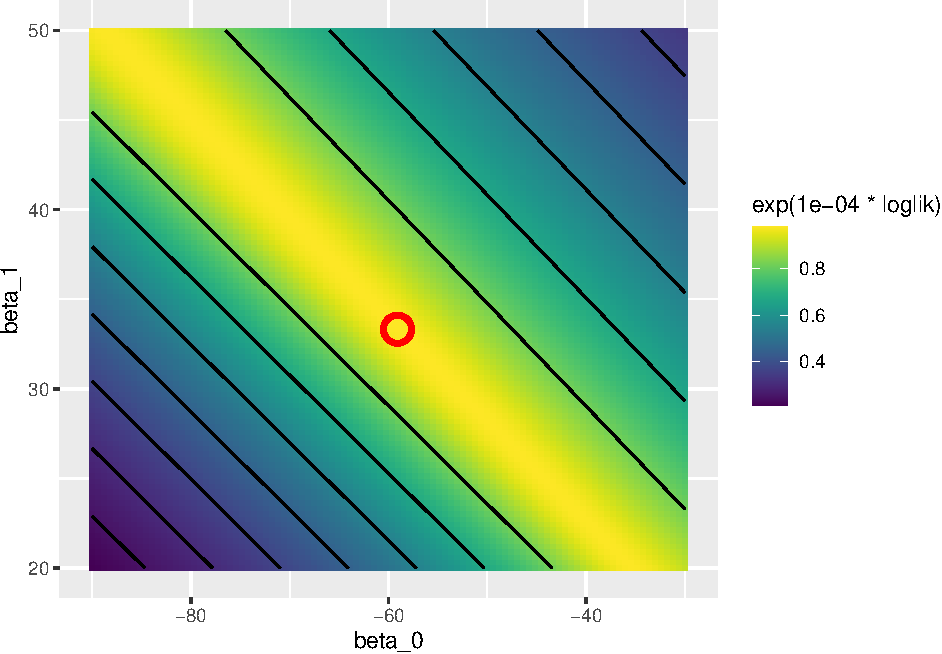
\includegraphics{3BinReg_files/figure-latex/unnamed-chunk-16-1.pdf}

Comments to the code: for the \texttt{loglik} function we have two
arguments: par= the parameters to be estimated, and args=a list with
data. The reason for only having these two arguments is that it is
easier to use when we later perform optimization (with \texttt{optim})
of the loglikelihood to find the ML estimates.

\begin{center}\rule{0.5\linewidth}{0.5pt}\end{center}

\hypertarget{problem-3-score-function}{%
\subsubsection{Problem 3: Score
function}\label{problem-3-score-function}}

\begin{enumerate}
\def\labelenumi{\alph{enumi})}
\tightlist
\item
  What is the definition of the score function? What is the dimension of
  the score function?
\item
  Derive the score function for the logit model (individual data). The
  result should be
  \[s(\boldsymbol{\beta})=\sum_{i=1}^n {\bf x}_i (y_i-\pi_i)=\sum_{i=1}^n {\bf x}_i (y_i-\frac{\exp({\bf x}_i^T\boldsymbol{\beta})}{1+\exp({\bf x}_i^T\boldsymbol{\beta})})\]
\item
  What do we need the score function for?
\end{enumerate}

\begin{center}\rule{0.5\linewidth}{0.5pt}\end{center}

\hypertarget{problem-4-fisher-information.}{%
\subsubsection{Problem 4: Fisher
information.}\label{problem-4-fisher-information.}}

(We did not cover this in the lecture week 1, but we know one of the
definitions from Module 2. Either you skip Problem 4 and move to Problem
5, or you look at the section \protect\hyperlink{propscore}{``Properties
of the score function''}, and \protect\hyperlink{covscore}{``The
expected Fisher information matrix \(F(\boldsymbol{\beta})\)''}
together.)

\begin{enumerate}
\def\labelenumi{\alph{enumi})}
\item
  What is the definition of the expected (and the observed) Fisher
  information matrix? What is the dimension of thise matrix (matrices)?
\item
  What is the role of these matrices in ML estimation?
\item
  For the logit model with grouped data the expected and the observed
  Fisher information matrix are equal and given as
\end{enumerate}

\[F(\boldsymbol{\beta})=\sum_{j=1}^G {\bf x}_j {\bf x}_j^T n_j \pi_j (1-\pi_j)\]
Where is \(\boldsymbol{\beta}\) in this expression?

\begin{enumerate}
\def\labelenumi{\alph{enumi})}
\setcounter{enumi}{3}
\tightlist
\item
  Write the version of the expected Fisher information for individual
  data (i.e.~\(n_j=1\) and \(G=n\)).
\end{enumerate}

\begin{center}\rule{0.5\linewidth}{0.5pt}\end{center}

\hypertarget{problem-5-maximum-likelihood}{%
\subsubsection{Problem 5: Maximum
likelihood}\label{problem-5-maximum-likelihood}}

To find the ML estimate for \(\boldsymbol{\beta}\) we may either use the
function \texttt{glm} or optimize the log-likelihood manually. We will
do both.

\begin{enumerate}
\def\labelenumi{\alph{enumi})}
\tightlist
\item
  First we use the \texttt{glm} function in R, and we also check that
  the individual and the grouped data give the same parameter estimates
  for the \(\boldsymbol{\beta}\). Read the R-code, notice the different
  input structures and check the results.
\end{enumerate}

\begin{Shaded}
\begin{Highlighting}[]
\CommentTok{\# the beetle.ds was made above}
\NormalTok{fitind}\OtherTok{=}\FunctionTok{glm}\NormalTok{(killed }\SpecialCharTok{\textasciitilde{}}\NormalTok{ ldose, }\AttributeTok{family =} \StringTok{"binomial"}\NormalTok{, }\AttributeTok{data =}\NormalTok{ beetleds) }\CommentTok{\# individual data}
\FunctionTok{summary}\NormalTok{(fitind)}
\end{Highlighting}
\end{Shaded}

\begin{verbatim}
## 
## Call:
## glm(formula = killed ~ ldose, family = "binomial", data = beetleds)
## 
## Coefficients:
##             Estimate Std. Error z value Pr(>|z|)    
## (Intercept)  -60.717      5.181  -11.72   <2e-16 ***
## ldose         34.270      2.912   11.77   <2e-16 ***
## ---
## Signif. codes:  0 '***' 0.001 '**' 0.01 '*' 0.05 '.' 0.1 ' ' 1
## 
## (Dispersion parameter for binomial family taken to be 1)
## 
##     Null deviance: 645.44  on 480  degrees of freedom
## Residual deviance: 372.47  on 479  degrees of freedom
## AIC: 376.47
## 
## Number of Fisher Scoring iterations: 5
\end{verbatim}

\begin{Shaded}
\begin{Highlighting}[]
\NormalTok{fitgrouped}\OtherTok{=}\FunctionTok{glm}\NormalTok{(}\FunctionTok{cbind}\NormalTok{(y, n}\SpecialCharTok{{-}}\NormalTok{y) }\SpecialCharTok{\textasciitilde{}}\NormalTok{ ldose, }\AttributeTok{family =} \StringTok{"binomial"}\NormalTok{, }\AttributeTok{data =}\NormalTok{ investr}\SpecialCharTok{::}\NormalTok{beetle) }\CommentTok{\# grouped data. response is \#success AND \#fails (here we have defined a dead beetle as a success)}
\FunctionTok{summary}\NormalTok{(fitgrouped)}
\end{Highlighting}
\end{Shaded}

\begin{verbatim}
## 
## Call:
## glm(formula = cbind(y, n - y) ~ ldose, family = "binomial", data = investr::beetle)
## 
## Coefficients:
##             Estimate Std. Error z value Pr(>|z|)    
## (Intercept)  -60.717      5.181  -11.72   <2e-16 ***
## ldose         34.270      2.912   11.77   <2e-16 ***
## ---
## Signif. codes:  0 '***' 0.001 '**' 0.01 '*' 0.05 '.' 0.1 ' ' 1
## 
## (Dispersion parameter for binomial family taken to be 1)
## 
##     Null deviance: 284.202  on 7  degrees of freedom
## Residual deviance:  11.232  on 6  degrees of freedom
## AIC: 41.43
## 
## Number of Fisher Scoring iterations: 4
\end{verbatim}

\begin{enumerate}
\def\labelenumi{\alph{enumi})}
\setcounter{enumi}{1}
\item
  What is the default convergence criterion for the glm? (Note: IRWLS
  used in \texttt{glm} - more in Module 5.)
\item
  We implemented the log-likelihood as a function in item 2 above. Now
  we will use this together with the \texttt{optim} function on the
  beetle data set to optimize the loglikelihood. Read the R-code, take
  notice of how we put data into the \texttt{args} slot and how the
  optimization is called with \texttt{optim}. (In Compulsory exercise 2
  you will use this in a Poisson regression.)
\end{enumerate}

\begin{Shaded}
\begin{Highlighting}[]
\NormalTok{loglik\_gr }\OtherTok{\textless{}{-}} \ControlFlowTok{function}\NormalTok{(par, args) \{}
    
\NormalTok{    y }\OtherTok{\textless{}{-}}\NormalTok{ args}\SpecialCharTok{$}\NormalTok{y}
\NormalTok{    x }\OtherTok{\textless{}{-}}\NormalTok{ args}\SpecialCharTok{$}\NormalTok{x}
\NormalTok{    n }\OtherTok{\textless{}{-}}\NormalTok{ args}\SpecialCharTok{$}\NormalTok{n}
    
\NormalTok{    res }\OtherTok{\textless{}{-}}\NormalTok{ y }\SpecialCharTok{\%*\%}\NormalTok{ x }\SpecialCharTok{{-}} \FunctionTok{t}\NormalTok{(}\FunctionTok{t}\NormalTok{(n }\SpecialCharTok{*}\NormalTok{ x) }\SpecialCharTok{\%*\%}\NormalTok{ ((}\DecValTok{1} \SpecialCharTok{+} \FunctionTok{exp}\NormalTok{(}\SpecialCharTok{{-}}\NormalTok{x }\SpecialCharTok{\%*\%}\NormalTok{ par))}\SpecialCharTok{\^{}}\NormalTok{(}\SpecialCharTok{{-}}\DecValTok{1}\NormalTok{)))}
    \FunctionTok{return}\NormalTok{(res)}
\NormalTok{\}}

\NormalTok{opt }\OtherTok{\textless{}{-}} \FunctionTok{optim}\NormalTok{(}\FunctionTok{c}\NormalTok{(}\SpecialCharTok{{-}}\DecValTok{60}\NormalTok{, }\DecValTok{30}\NormalTok{), }\AttributeTok{fn =}\NormalTok{ loglik, }\AttributeTok{gr =}\NormalTok{ loglik\_gr, }\AttributeTok{args =} \FunctionTok{list}\NormalTok{(}\AttributeTok{y =}\NormalTok{ beetleds}\SpecialCharTok{$}\NormalTok{killed, }
    \AttributeTok{x =} \FunctionTok{cbind}\NormalTok{(}\FunctionTok{rep}\NormalTok{(}\DecValTok{1}\NormalTok{, }\FunctionTok{nrow}\NormalTok{(beetleds)), beetleds}\SpecialCharTok{$}\NormalTok{ldose), }\AttributeTok{n =} \FunctionTok{rep}\NormalTok{(}\DecValTok{1}\NormalTok{, }\FunctionTok{nrow}\NormalTok{(beetleds))), }
    \AttributeTok{control =} \FunctionTok{list}\NormalTok{(}\AttributeTok{fnscale =} \SpecialCharTok{{-}}\DecValTok{1}\NormalTok{), }\AttributeTok{hessian =} \ConstantTok{TRUE}\NormalTok{,}\AttributeTok{method=}\StringTok{"BFGS"}\NormalTok{)}
\NormalTok{opt }
\end{Highlighting}
\end{Shaded}

\begin{verbatim}
## $par
## [1] -60.71748  34.27034
## 
## $value
## [1] -186.2354
## 
## $counts
## function gradient 
##       24        9 
## 
## $convergence
## [1] 0
## 
## $message
## NULL
## 
## $hessian
##            [,1]      [,2]
## [1,]  -58.48417 -104.0105
## [2,] -104.01047 -185.0941
\end{verbatim}

\begin{Shaded}
\begin{Highlighting}[]
\FunctionTok{sqrt}\NormalTok{(}\FunctionTok{diag}\NormalTok{(}\SpecialCharTok{{-}}\FunctionTok{solve}\NormalTok{(opt}\SpecialCharTok{$}\NormalTok{hessian))) }\CommentTok{\# calculate the standard deviations of the parameters}
\end{Highlighting}
\end{Shaded}

\begin{verbatim}
## [1] 5.180709 2.912138
\end{verbatim}

\begin{center}\rule{0.5\linewidth}{0.5pt}\end{center}

\hypertarget{problem-6-interpreting-results}{%
\subsubsection{Problem 6: Interpreting
results}\label{problem-6-interpreting-results}}

\begin{enumerate}
\def\labelenumi{\alph{enumi})}
\tightlist
\item
  Interpret the estimated \(\boldsymbol{\beta}\)´s. Odds ratio is useful
  for this.
\item
  Plot the predicted probability of a beetle dying against the dosage
  and discuss what you see. (Yes, since this is the last question you
  may try to program by yourself!)
\end{enumerate}

\begin{center}\rule{0.5\linewidth}{0.5pt}\end{center}

\textbf{SECOND WEEK}

Remember the \protect\hyperlink{beetle1}{beetle} and
\protect\hyperlink{infant1}{infant respitory disease} examples?

First, we look back at the \protect\hyperlink{binaryregassump}{model
requirements} for the binary regression - and the
\protect\hyperlink{loglik}{loglikelihood} and
\protect\hyperlink{score}{score function}.

\begin{center}\rule{0.5\linewidth}{0.5pt}\end{center}

\hypertarget{likelihood-and-derivations-thereof---continued}{%
\section{Likelihood and derivations thereof -
continued}\label{likelihood-and-derivations-thereof---continued}}

Individual data (not grouped):

Loglikelihood:
\[l(\boldsymbol{\beta})=\sum_{i=1}^n[y_i \ln \pi_i-y_i\ln(1-\pi_i)+\ln(1-\pi_i)]\]

Score function:
\[s(\boldsymbol{\beta})=\sum_{i=1}^n {\bf x}_i (y_i-\pi_i)\]

\begin{center}\rule{0.5\linewidth}{0.5pt}\end{center}

\hypertarget{properties-of-the-score-function}{%
\subsection{Properties of the score
function}\label{properties-of-the-score-function}}

Since the score function depends on \(Y_i=y_i\) we may regard the score
function as a random vector. We will now calculate the mean and
covariance matrix for the score function. The expected value is

\[E(s(\boldsymbol{\beta})) = E(\sum_{i=1}^n(Y_i-\pi_i){\bf x}_i) = \sum_{i=1}^nE((Y_i-\pi_i){\bf x}_i) = \sum_{i=1}^n(E(Y_i)-\pi_i){\bf x}_i = 0 \]

as \(E(Y_i) = \pi_i\). We also see that
\(E(s_i(\boldsymbol{\beta})) = E((Y_i-\pi_i){\bf x}_i) = 0 \ \forall i\).

\begin{center}\rule{0.5\linewidth}{0.5pt}\end{center}

\hypertarget{the-expected-fisher-information-matrix-fboldsymbolbeta}{%
\subsection{\texorpdfstring{The expected Fisher information matrix
\(F(\boldsymbol{\beta})\)}{The expected Fisher information matrix F(\textbackslash boldsymbol\{\textbackslash beta\})}}\label{the-expected-fisher-information-matrix-fboldsymbolbeta}}

The covariance of \(s(\boldsymbol{\beta})\) is called the expected
Fisher information matrix, \(F(\boldsymbol{\beta})\) and is given by

\begin{align} F(\boldsymbol{\beta}) &= \text{Cov}(s(\boldsymbol{\beta})) =   \sum_{i=1}^n \text{Cov}(s_i(\boldsymbol{\beta})) \\
&= \sum_{i=1}^n E\left[\Big(s_i(\boldsymbol{\beta}) - E(s_i(\boldsymbol{\beta}))\Big)\Big(s_i(\boldsymbol{\beta})-E(s_i(\boldsymbol{\beta}))\Big)^T\right] \\
&= \sum_{i=1}^n E(s_i(\boldsymbol{\beta})s_i(\boldsymbol{\beta})^T) = \sum_{i=1}^n F_i(\boldsymbol{\beta}) 
\end{align}

where it is used that the responses \(Y_i\) and \(Y_j\) are independent,
and that \(E(s_i(\boldsymbol{\beta})) = 0 \ \forall i\).

\begin{center}\rule{0.5\linewidth}{0.5pt}\end{center}

Remember that \(s_i(\boldsymbol{\beta})=(Y_i-\pi_i){\bf x}_i\), then:

\[ F_i(\boldsymbol{\beta}) = E(s_i(\boldsymbol{\beta})s_i(\boldsymbol{\beta})^T) = E((Y_i-\pi_i){\bf x}_i(Y_i-\pi_i){\bf x}_i^T) \]
\[= {\bf x}_i{\bf x}_i^T E((Y_i-\pi_i)^2) = {\bf x}_i{\bf x}_i^T \pi_i(1-\pi_i) \]
where \(E((Y_i-\pi_i)^2)=\text{Var}(Y_i)=\pi_i(1-\pi_i)\) is the
variance of \(Y_i\). Thus

\[F(\boldsymbol{\beta}) = \sum_{i=1}^n {\bf x}_i{\bf x}_i^T \pi_i(1-\pi_i).\]

\begin{center}\rule{0.5\linewidth}{0.5pt}\end{center}

\textbf{A useful relationship:} Under mild regularity conditions (so we
can change the order of \(\int\) and
\(\frac{\partial}{\partial \boldsymbol{\beta}}\)):

\[\text{Cov}(s(\boldsymbol{\beta})=F(\boldsymbol{\beta}) = E\left( -\frac{\partial^2l(\boldsymbol{\beta})}{\partial\boldsymbol{\beta}\partial\boldsymbol{\beta}^T} \right) = E(-\text{Hessian matrix of }l)\]
which relates the expected to the observed Fisher information matrix.

\href{ExpectedFisherinfo.pdf}{Do you want to see an explanation?}

\begin{center}\rule{0.5\linewidth}{0.5pt}\end{center}

\hypertarget{observed-fisher-information-matrix-hboldsymbolbeta}{%
\subsection{\texorpdfstring{Observed Fisher information matrix
\(H(\boldsymbol{\beta})\)}{Observed Fisher information matrix H(\textbackslash boldsymbol\{\textbackslash beta\})}}\label{observed-fisher-information-matrix-hboldsymbolbeta}}

\[H(\boldsymbol{\beta}) = -\frac{\partial^2l(\boldsymbol{\beta})}{\partial\boldsymbol{\beta}\partial\boldsymbol{\beta}^T} = -\frac{\partial s(\boldsymbol{\beta})}{\partial\boldsymbol{\beta}^T} = \frac{\partial}{\partial\boldsymbol{\beta}^T}\left[\sum_{i=1}^n (\pi_i-y_i){\bf x}_i \right] \]

because \(s(\boldsymbol{\beta}) = \sum_{i=1}^n (y_i-\pi_i){\bf x}_i\)
and hence
\(-s(\boldsymbol{\beta}) = \sum_{i=1}^n (\pi_i-y_i){\bf x}_i\). Note
that \(\pi_i = \pi_i(\boldsymbol{\beta})\).

\[H(\boldsymbol{\beta}) = \sum_{i=1}^n \frac{\partial}{\partial\boldsymbol{\beta}^T}[{\bf x}_i\pi_i-{\bf x}_iy_i] = \sum_{i=1}^n \frac{\partial}{\partial\boldsymbol{\beta}^T}{\bf x}_i\pi_i = \sum_{i=1}^n {\bf x}_i \frac{\partial \pi_i}{\partial \eta_i} \frac{\partial \eta_i}{\partial \boldsymbol{\beta}^T} \]

\begin{center}\rule{0.5\linewidth}{0.5pt}\end{center}

Use that

\[ \frac{\partial \eta_i}{\partial \boldsymbol{\beta}^T}=\frac{\partial {\bf x}_i^T\boldsymbol{\beta}}{\partial \boldsymbol{\beta}^T} = \left(\frac{\partial {\bf x}_i^T\boldsymbol{\beta}}{\partial \boldsymbol{\beta}}\right)^T = {\bf x}_i^T \]

and

\[ \frac{\partial \pi_i}{\partial \eta_i} =  \frac{\partial\left(\frac{\exp(\eta_i)}{1+\exp(\eta_i)}\right)}{\partial \eta_i} = \frac{(1+\exp(\eta_i))\exp(\eta_i) - \exp(\eta_i)\exp(\eta_i)}{(1+\exp(\eta_i))^2} \]
\[=\pi_i (1-\pi_i).\]

\begin{center}\rule{0.5\linewidth}{0.5pt}\end{center}

And thus

\[H(\boldsymbol{\beta}) =\sum_{i=1}^n {\bf x}_i\pi_i(1-\pi_i) {\bf x}_i^T = \sum_{i=1}^n {\bf x}_i{\bf x}_i^T \pi_i(1-\pi_i).\]
Note that the observed and the expected Fisher information matrix are
equal (see below - canonical link - that this is a general finding).
This is not the case for the probit or complementary log-log models.

\begin{center}\rule{0.5\linewidth}{0.5pt}\end{center}

\hypertarget{overview-of-the-results-for-individual-and-grouped-data}{%
\subsection{Overview of the results for individual and grouped
data}\label{overview-of-the-results-for-individual-and-grouped-data}}

\begin{itemize}
\tightlist
\item
  Individual data: \(i=1,\ldots, n\), and pairs \(({\bf x}_i,y_i)\).
\item
  Grouped data: \(j=1,\ldots, G\) with \(n_j\) observations for group
  \(j\), and \(Y_j=\sum Y_i\) for all \(i\) member of group \(j\). In
  total \(\sum_{j=1}^G n_j\) observations. For each pair
  \(({\bf x}_j, y_j)\), where \({\bf x}_j\) the covariate pattern for
  group \(j\).
\end{itemize}

NB: we keep that \(\eta_i=\ln (\frac{\pi_i}{1-\pi_i})\) - not changed
for grouped data (but now \(\mu_j=n_j\pi_j\)).

\begin{center}\rule{0.5\linewidth}{0.5pt}\end{center}

\textbf{Log-likelihood:}

Individual:
\[l(\boldsymbol{\beta})=\sum_{i=1}^n[y_i \ln \pi_i-y_i\ln(1-\pi_i)+\ln(1-\pi_i)]\]
Grouped:
\[l(\boldsymbol{\beta})=\sum_{j=1}^G[y_j \ln \pi_j-y_j\ln(1-\pi_j)+n_j\ln(1-\pi_j)+ \ln {n_j \choose y_j}]\]
The last part is usually not include in calculations.

\begin{center}\rule{0.5\linewidth}{0.5pt}\end{center}

\textbf{Score function:}

Individual: \[s(\boldsymbol{\beta})=\sum_{i=1}^n {\bf x}_i (y_i-\pi_i)\]

Grouped: \[s(\boldsymbol{\beta})=\sum_{j=1}^G {\bf x}_j (y_j-n_j\pi_j)\]

\begin{center}\rule{0.5\linewidth}{0.5pt}\end{center}

\textbf{Expected Fisher information matrix:}

Individual:

\[F(\boldsymbol{\beta})=\sum_{i=1}^n {\bf x}_i {\bf x}_i^T\pi_i (1-\pi_i)\]

Grouped:

\[F(\boldsymbol{\beta})=\sum_{j=1}^G {\bf x}_j {\bf x}_j^T n_j \pi_j (1-\pi_j)\]

The observed Fisher information matrix equals the expected Fisher
information matrix - because the logit model is the \emph{canonical
link} for the binomial distribution.

\begin{center}\rule{0.5\linewidth}{0.5pt}\end{center}

\hypertarget{look-back-at-mlr---what-is-sboldsymbolbeta-and-fboldsymbolbeta-then}{%
\subsection{\texorpdfstring{Look back at MLR - what is
\(s(\boldsymbol{\beta})\) and \(F(\boldsymbol{\beta})\)
then?}{Look back at MLR - what is s(\textbackslash boldsymbol\{\textbackslash beta\}) and F(\textbackslash boldsymbol\{\textbackslash beta\}) then?}}\label{look-back-at-mlr---what-is-sboldsymbolbeta-and-fboldsymbolbeta-then}}

\begin{enumerate}
\def\labelenumi{\arabic{enumi}.}
\item
  \(Y_i \sim \text{N}(\mu_i, \sigma^2)\)
\item
  \(\eta_j = x_i^T\boldsymbol{\beta}\)
\item
  \(\mu_i = \eta_i\) (identity response function and link function)
\end{enumerate}

Likelihood:

\[L(\boldsymbol{\beta}) = \left(\frac{1}{2\pi}\right)^{n/2}\left(\frac{1}{\sigma^2}\right)^{n/2} \exp\left(-\frac{1}{2\sigma^2}(y-{\bf X}\boldsymbol{\beta})^T(y-{\bf X}\boldsymbol{\beta})\right)\]

Loglikelihood:
\[l(\boldsymbol{\beta}) = \ln L(\boldsymbol{\beta}) = -\frac{n}{2} \ln (2\pi) - \frac{n}{2} \ln (\sigma^2) - \frac{1}{2\sigma^2}(y-{\bf X}\boldsymbol{\beta})^T(y-{\bf X}\boldsymbol{\beta})\]

\begin{center}\rule{0.5\linewidth}{0.5pt}\end{center}

Since
\((y-{\bf X}\boldsymbol{\beta})^T(y-{\bf X}\boldsymbol{\beta}) = Y^TY - 2Y^T{\bf X}\boldsymbol{\beta} + \boldsymbol{\beta}^T{\bf X}^T{\bf X}\boldsymbol{\beta}\),
then

\[s(\boldsymbol{\beta}) = \frac{\partial l(\boldsymbol{\beta})}{\partial \boldsymbol{\beta}} = -\frac{1}{2\sigma^2}(2{\bf X}^T{\bf X}\boldsymbol{\beta}-2{\bf X}^TY) = \frac{1}{\sigma^2}({\bf X}^TY - {\bf X}^T{\bf X}\boldsymbol{\beta})\]

and \(s(\hat{\boldsymbol{\beta}}) = 0\) gives
\({\bf X}^TY - {\bf X}^T{\bf X}\boldsymbol{\beta} = 0\) which can be
solved on closed form giving
\(\hat{\boldsymbol{\beta}} = ({\bf X}^T{\bf X})^{-1}{\bf X}^TY\). So, no
need for iterative methods.

\begin{center}\rule{0.5\linewidth}{0.5pt}\end{center}

Finally, observed Fisher information matrix.

\[H(\boldsymbol{\beta}) = \frac{\partial s(\boldsymbol{\beta})}{\partial \boldsymbol{\beta}^T} = -\frac{\partial}{\partial \boldsymbol{\beta}_T}(\frac{1}{\sigma^2}{\bf X}^TY - \frac{1}{\sigma^2}{\bf X}^T{\bf X}\boldsymbol{\beta}) = \frac{1}{\sigma^2}{\bf X}^T{\bf X}\]

which is independent on \(\boldsymbol{\beta}\), and also we see that
\(F(\boldsymbol{\beta})=\text{E}(H(\boldsymbol{\beta}))=H(\boldsymbol{\beta})\)
since no random variables are present. The identity link is also the
canonical link. Finally, the (asymptotic) covariance of the ML estimate
is \(F^{-1}(\hat{\boldsymbol{\beta}})=({\bf X}^T{\bf X})^{-1}\sigma^2\)
which we know as \(\text{Cov}(\hat{\boldsymbol{\beta}})\).

\hypertarget{exponential-family---and-canonical-link}{%
\section{Exponential family - and canonical
link}\label{exponential-family---and-canonical-link}}

In Module 1 we introduced distributions of the \(Y_i\), that could be
written in the form of a \emph{univariate exponential family}
\[ f(y_i\mid \theta_i)=\exp \left( \frac{y_i \theta_i-b(\theta_i)}{\phi}\cdot w_i + c(y_i, \phi, w_i) \right) \]
where

\begin{itemize}
\item
  \(\theta_i\) is called the canonical parameter and is a parameter of
  interest
\item
  \(\phi\) is called a nuisance parameter (and is not of interest to
  us=therefore a nuisance (plage))
\item
  \(w_i\) is a weight function, in most cases \(w_i=1\)
\item
  \(b\) and \(c\) are known functions.
\end{itemize}

It can be shown that \(\text{E}(Y_i)=b'(\theta_i)\) and
\(\text{Var}(Y_i)=b''(\theta_i)\cdot \frac{\phi}{w_i}\).

\begin{center}\rule{0.5\linewidth}{0.5pt}\end{center}

In Module 1 we found that the binomial distribution
\(Y_i\sim \text{bin}(1,\pi_i)\) is an exponential family (derivation
from Module 1:
\url{https://www.math.ntnu.no/emner/TMA4315/2017h/Module1ExponentialFamily.pdf})

and that

\begin{itemize}
\tightlist
\item
  \(\theta_i=\ln( \frac{\pi_i}{1-\pi_i})\) is the canonical parameter
\item
  \(\phi=1\), no nuisance
\item
  \(w_i=1\)
\item
  \(b(\theta_i)=\ln(1+\exp(\theta_i))\)
\end{itemize}

\begin{center}\rule{0.5\linewidth}{0.5pt}\end{center}

Recall that in a GLM we choose a link function \(g\), linking the linear
predictor and the mean: \(\eta_i=g(\mu_i)\). For the logit model we had
that \(\eta_i=\ln(\frac{\pi_i}{1-\pi_i})\).

Now (new to us) - every exponential family has a unique \emph{canonical
link function} such that \[\theta_i=\eta_i\] Since \(\eta_i=g(\mu_i)\)
this means to us that we need \[ g(\mu_i)=\theta_i\] to have a canonical
link.

\textbf{Q:} Is the logit link the canonical link for the binary model?

\textbf{A}:

Yes, since \(\theta_i=\ln( \frac{\pi_i}{1-\pi_i})=g(\pi_i)\) then the
logit link is the canonical link for the binary regression.

\begin{center}\rule{0.5\linewidth}{0.5pt}\end{center}

\#\#Properties of a GLM with canonical link

\begin{enumerate}
\def\labelenumi{\arabic{enumi}.}
\item
  The log-likelihod is always concave so that the ML estimated is always
  unique (given that it exists).
\item
  The observed Fisher information matrix \(H(\boldsymbol{\beta})\)
  \emph{equals} the expected Fisher information matrix
  \(F(\boldsymbol{\beta})\). That is,
  \[-\frac{\partial^2 l}{\partial \boldsymbol{\beta} \boldsymbol{\beta}^T}=\text{E}(-\frac{\partial^2 l}{\partial \boldsymbol{\beta} \boldsymbol{\beta}^T})\]
\end{enumerate}

Proving this is beyond the scope of this course.

\hypertarget{parameter-estimation---in-practise}{%
\section{Parameter estimation - in
practise}\label{parameter-estimation---in-practise}}

To find the ML estimate \(\hat{\boldsymbol{\beta}}\) we need to solve
\[s(\hat{\boldsymbol{\beta}})=0\] We have that the score function for
the logit model is:
\[s(\boldsymbol{\beta})=\sum_{j=1}^G {\bf x}_j (y_j-n_j\pi_j)\] where
\(\pi_j=\frac{\exp({\bf x}_j^T\hat{\boldsymbol{\beta}})}{1+\exp({\bf x}_j^T\hat{\boldsymbol{\beta}})}\).
Observe that this is a non-linear function in \(\boldsymbol{\beta}\),
and has no closed form solution.

\begin{center}\rule{0.5\linewidth}{0.5pt}\end{center}

\#\#Iterative gradient-based methods

Back to the general case - we may use a first order multivariate Taylor
approximation for \(s(\hat{\boldsymbol{\beta}})\), around some chosen
reference value \(\boldsymbol{\beta}^{(0)}\):
\[s(\hat{\boldsymbol{\beta}})\approx s(\boldsymbol{\beta}^{(0)})+\frac{\partial s(\boldsymbol{\beta})}{\partial \boldsymbol{\beta}}\big\rvert_{\boldsymbol{\beta}=\boldsymbol{\beta}^{(0)}} (\hat{\boldsymbol{\beta}}-\boldsymbol{\beta}^{(0)})\]

Let
\(H(\boldsymbol{\beta}^{(0)})=-\frac{\partial s(\boldsymbol{\beta})}{\partial \boldsymbol{\beta}}\big\rvert_{\boldsymbol{\beta}=\boldsymbol{\beta}^{(0)}}\).
Setting \(s(\hat{\boldsymbol{\beta}})=0\) solving for
\(\hat{\boldsymbol{\beta}}\) gives
\[ \hat{\boldsymbol{\beta}}=\boldsymbol{\beta}^{(0)} + H(\boldsymbol{\beta}^{(0)})^{-1} s(\boldsymbol{\beta}^{(0)})\]
where \(H(\boldsymbol{\beta}^{(0)})^{-1}\) is the matrix inverse of
\(H(\boldsymbol{\beta}^{(0)})\).

If we start with some value \(\boldsymbol{\beta}^{(0)}\) and then find a
new value \(\boldsymbol{\beta}^{(1)}\) by applying this equation, and
then continue applying the equation until convergence we have the
\emph{Newton-Raphson} method:

\[\boldsymbol{\beta}^{(t+1)}=\boldsymbol{\beta}^{(t)} + H(\boldsymbol{\beta}^{(t)})^{-1} s(\boldsymbol{\beta}^{(t)})\]

\begin{center}\rule{0.5\linewidth}{0.5pt}\end{center}

Replacing the observed Fisher information matrix \({\bf H}\) with the
expected Fisher information matrix \({\bf F}\) yields the
\emph{Fisher-scoring} method.

For the logit model these two methods are the same since the observed
and expected Fisher information matrix is the same for canonical link
functions (like the logit is for binary regression).

This algorithm is run until the relative difference in Euclidean
distance between two iterations ``(new-old)/old'' is smaller than some
chosen constant.

\begin{center}\rule{0.5\linewidth}{0.5pt}\end{center}

\#\#Requirements for convergence

For the Newton-Raphson algorithm we see that the observed Fisher
information matrix \(H\) needs to be invertible for all
\(\boldsymbol{\beta}\), alternatively for the Fisher scoring algorithm
the expected Fisher information matrix \(F\) needs to be invertible.

In our logit model
\[F(\boldsymbol{\beta})=\sum_{j=1}^G {\bf x}_j {\bf x}_j^T n_j \pi_j (1-\pi_j)\]

Let \({\bf X}\) be the design matrix, where the rows are
\({\bf x}_j^T\). Then
\({\bf X}^T{\bf X}=\sum_{j=1}^G {\bf x}_j {\bf x}_j^T\).

If we require that the design matrix has full rank (\(G\)) then also
\({\bf X}^T{\bf X}\) will have full rank (it will also be positive
definite) and and in addition \(\pi_j(1-\pi_j)>0\) for all
\(\pi_j \in (0,1)\), so then \(F(\boldsymbol{\beta})\) will be positive
definite and all is good.

\begin{center}\rule{0.5\linewidth}{0.5pt}\end{center}

\textbf{Why is \(F(\boldsymbol{\beta})\) positive definite if we require
that the design matrix has full rank?} Formally, let \({\bf X}\) be a
\(n\times p\) matrix and \(\Lambda\) a \(n\times n\) diagonal matrix
where all the diagonal elements are positive (like our
\(\pi_j(1-\pi_j)\), yes, put them on the diagonal). Let \({\bf X}\) have
independent columnes (full rank) \(\Leftrightarrow\)
\({\bf X}^T\Lambda{\bf X}\) is positive definite.

\emph{Proof:} \(\Rightarrow\): Let \({\bf v}\) be a \(p\) dimensional
column vector. Assume
\(0={\bf v}^T {\bf X}^T \Lambda {\bf X} {\bf v}=(\Lambda^{1/2}{\bf X}{\bf v})^T(\Lambda^{1/2}{\bf X}{\bf v})=\sum_{i=1}^n w_i^2\)
where \({\bf W}=\Lambda^{1/2}{\bf X}{\bf v}\). Then, \(w\) must be 0,
that is \(\Lambda^{1/2}{\bf X}{\bf v}=0\) since multiplication with
\(\Lambda^{1/2}\) is to multiply each element in \({\bf X}{\bf v}\) with
a number different from 0. That is, we must have \({\bf v}={\bf 0}\)
since \({\bf X}\) has independent columns.

\(\Leftarrow\): Assume that \({\bf X}{\bf v}={\bf 0}\). Then
\({\bf v}^T {\bf X}^T \Lambda {\bf X} {\bf v}={\bf 0}\) so
\({\bf v}={\bf 0}\) since \({\bf X}^T\Lambda{\bf X}\) is positive
definite. This is, \({\bf X}\) has independent columns.

\emph{End of proof}

\begin{center}\rule{0.5\linewidth}{0.5pt}\end{center}

Therefore, for GLMs we will also - as for the multiple linear regression
model in Module 2 - assume that the design matrix has full rank!

We will see in Module 5 that this is the requirement needed for GLMs in
general.

However, it is possible that the algorithm does not converge. This may
happen for ``unfavorable'' data configurations (especially for small
samples). Accoring to our text book, Fahrmeir et al (2013), page 284,
the conditions for uniqueness and existence of ML estimators are very
complex, and the authors suggest that the GLM user instead checks for
convergence in practice by performing the iterations.

\hypertarget{asymptotic-properties-of-ml-estimates}{%
\section{Asymptotic properties of ML
estimates}\label{asymptotic-properties-of-ml-estimates}}

\hypertarget{results}{%
\subsection{Results}\label{results}}

Under some (weak) regularity conditions (including that
\(\boldsymbol{\beta}\) falls in the interior of the parameter space and
\(p\) is fixed that \(n\) increases, Agresti (2015) page 125):

Let \(\hat{\boldsymbol{\beta}}\) be the maximum likelihood (ML) estimate
in the GLM model. As the total sample size increases,
\(n\rightarrow \infty\):

\begin{enumerate}
\def\labelenumi{\arabic{enumi}.}
\tightlist
\item
  \(\hat{\boldsymbol{\beta}}\) exists
\item
  \(\hat{\boldsymbol{\beta}}\) is consistent (convergence in
  probability, yielding asymptotically unbiased estimator, variances
  goes towards 0)
\item
  \(\hat{\boldsymbol{\beta}} \approx N_p(\boldsymbol{\beta},F^{-1}(\hat{\boldsymbol{\beta}}))\)
\end{enumerate}

Observe that this means that asymptotically
\(\text{Cov}(\hat{\boldsymbol{\beta}})=F^{-1}(\hat{\boldsymbol{\beta}})\):
the inverse of the expected Fisher information matrix evaluated at the
ML estimate.

Observe: The result requires that the \emph{total} sample size goes to
infinity (not the individual \(n_j\) for the covariate patterns).

\begin{center}\rule{0.5\linewidth}{0.5pt}\end{center}

The \emph{proof} (for the univariate case) is given in the course
TMA4295 Statistical Inference course, Casella and Berger
(2002):``Statistical inference'', page 472. It starts by a first order
Taylor expansion of the score function (derivative of loglikelihood)
around the true parameter, and utilizes the fact that the maximum
likelihood estimate is defined as the zero of the score function.

\begin{center}\rule{0.5\linewidth}{0.5pt}\end{center}

The following is not a formal proof, but a sketch - and I use the
parameter of interest \(\boldsymbol{\theta}\) in the exponential family
version of the distribution (and then there is a connection to the mean
\(\boldsymbol{\mu}\) and then to \(\boldsymbol{\eta}\) and finally
\(\boldsymbol{\beta}\)):

We start with the multivariate version of the first order Taylor
expansion around the true parameter value \(\boldsymbol{\theta}\):

\[{\bf 0}=s(\hat{\boldsymbol{\theta}})\approx s({\boldsymbol{\theta}})-{\bf H}({\boldsymbol{\theta}})(\hat{\boldsymbol{\theta}}-{\boldsymbol{\theta}})\]

We assume that \(\hat{\boldsymbol{\theta}}\) is the maximum likelihood
estimate, and there the score function is \({\bf 0}\) so we get:
\[s({\boldsymbol{\theta}})\approx {\bf H}({\boldsymbol{\theta}})(\hat{\boldsymbol{\theta}}-{\boldsymbol{\theta}})\]
And premultiplying with \({\bf H}^{-1}(\boldsymbol{\theta})\) gives
\[ (\hat{\boldsymbol{\theta}}-{\boldsymbol{\theta}})\approx {\bf H}^{-1}({\boldsymbol{\theta}})s({\boldsymbol{\theta}})\]
Then, to use the central limit theorem we need some smart manipulations
with \(n\), so we start by multiplying with \(\sqrt{n}\) and split that
into \(n\) and \(\frac{1}{\sqrt{n}}\).

\begin{center}\rule{0.5\linewidth}{0.5pt}\end{center}

\[ \sqrt{n}(\hat{\boldsymbol{\theta}}-{\boldsymbol{\theta}})\approx \sqrt{n}{\bf H}^{-1}({\boldsymbol{\theta}})s({\boldsymbol{\theta}})=(\frac{1}{n}{\bf H}({\boldsymbol{\theta}}))^{-1}\frac{1}{\sqrt{n}}s({\boldsymbol{\theta}})\]

From the central limit theorem:

\begin{enumerate}
\def\labelenumi{\arabic{enumi})}
\item
  \(\frac{1}{n}{\bf H}(\boldsymbol{\theta})\) goes to the expected value
  which is \({\bf F}(\boldsymbol{\theta})\) (in probability),
\item
  the part \(\frac{1}{\sqrt{n}}s({\boldsymbol{\theta}})\) asymptoticalle
  goes to a random variable \(W\) that follows a multivariate normal
  with

  \begin{itemize}
  \tightlist
  \item
    mean
    \(\text{E}(\frac{1}{\sqrt{n}}s({\boldsymbol{\theta}}))={\bf 0}\) and
    the
  \item
    covariance matrix is
    \(\text{Cov}(\frac{1}{\sqrt{n}}s({\boldsymbol{\theta}}))=\frac{1}{n}{\bf F}(\boldsymbol{\theta})\)
  \end{itemize}
\end{enumerate}

\[ {\bf W} \sim N({\bf 0},\frac{1}{n}{\bf F}(\boldsymbol{\theta}))\]

\begin{center}\rule{0.5\linewidth}{0.5pt}\end{center}

\[\sqrt{n}(\hat{\boldsymbol{\theta}}-{\boldsymbol{\theta}}) \approx \bf{F}^{-1}(\boldsymbol{\theta}){\bf W}\]

On the right side here we have a multivariate normal distributed random
variable \(\bf{F}^{-1}(\boldsymbol{\theta}){\bf W}\) with mean
\({\bf 0}\) and covariance matrix
\[\text{Cov}({\bf F}^{-1}(\boldsymbol{\theta}){\bf W})={\bf F}^{-1}(\boldsymbol{\theta})\frac{1}{n}{\bf F}(\boldsymbol{\theta}){\bf F}^{-1}(\boldsymbol{\theta})=\frac{1}{n}{\bf F}^{-1}(\boldsymbol{\theta})\]

This leads to the wanted result:

\[ \hat{\boldsymbol{\theta}}\approx N(\boldsymbol{\theta},{\bf F}^{-1}(\boldsymbol{\theta}))\]

Due to the Slutsky theorem (from TMA4295 Statistical inference) this
also holds when \({\bf F}^{-1}(\boldsymbol{\theta}))\) is replaced by
\({\bf F}^{-1}(\hat{\boldsymbol{\theta}}))\).

\begin{center}\rule{0.5\linewidth}{0.5pt}\end{center}

\hypertarget{parameter-estimation}{%
\section{Parameter estimation}\label{parameter-estimation}}

Parameter estimation can be based on grouped data - so now we use
\(Y_j \sim \text{bin}(n_j,\pi_j)\) from 1 above, but keep 2 and 3
unchanged. The number of groups is \(G\) and the total number of
observations is \(\sum_{j=1}^G n_j\).

\begin{itemize}
\item
  Likelihood=joint distribution, exponential family.
  \[ f(y\mid \theta)=\exp \left( \frac{y \theta-b(\theta)}{\phi}\cdot w + c(y, \phi, w) \right) \]
  where we have that \(\theta=\ln(\frac{\pi}{1-\pi})\) for the binomial
  distribution, which means that our logit model is gives the canonical
  link (remember, good properties!).
\item
  Log-likelihood
  \[l(\boldsymbol{\beta})=\sum_{j=1}^G[y_j \ln \pi_j-y_j\ln(1-\pi_j)+n_j\ln(1-\pi_j)+ \ln {n_j \choose y_j}]\]
\end{itemize}

\begin{center}\rule{0.5\linewidth}{0.5pt}\end{center}

\begin{itemize}
\item
  Score function=vector of partial derivatives of log-likelihood. Find
  ML by solving \(s(\hat{\boldsymbol{\beta})})=0\) - but no closed form
  solutions.
  \[s(\boldsymbol{\beta})=\sum_{j=1}^G {\bf x}_j (y_j-n_j\pi_j)\]
\item
  Expected Fisher information matrix
  \[F(\boldsymbol{\beta})=\sum_{j=1}^G {\bf x}_j {\bf x}_j^T n_j \pi_j (1-\pi_j)\]
\item
  \(\hat{\boldsymbol{\beta}}\) found iteratively using Newton-Raphson or
  Fisher scoring
  \[\boldsymbol{\beta}^{(t+1)}=\boldsymbol{\beta}^{(t)} + F(\boldsymbol{\beta}^{(t)})^{-1} s(\boldsymbol{\beta}^{(t)})\]
\item
  \(\hat{\boldsymbol{\beta}} \approx N_p(\boldsymbol{\beta},F^{-1}(\hat{\boldsymbol{\beta}}))\)
\end{itemize}

\hypertarget{further-statistical-inference}{%
\section{Further statistical
inference}\label{further-statistical-inference}}

Our further statistical inference (confidence intervals and hypotheses
tests) are based on the asymptotic distribution of the parameter
estimates
\[\hat{\boldsymbol{\beta}} \approx N_p(\boldsymbol{\beta},F^{-1}(\hat{\boldsymbol{\beta}}))\]
where \(F^{-1}(\hat{\boldsymbol{\beta}}))\) is the inverse of the
expected Fisher information matrix inserted
\(\hat{\boldsymbol{\beta}}\).

For the logit model we found that
\[F(\boldsymbol{\beta})=\sum_{j=1}^G {\bf x}_j {\bf x}_j^T n_j \pi_j (1-\pi_j)\]
So we would need to do \(\pi_j=\frac{\exp(\eta-j)}{1+\exp(\eta_j)}\) and
\(\eta_j={\bf x}_j^T\boldsymbol{\beta}\) as ``usual'', and then replace
\(\boldsymbol{\beta}\) with \(\hat{\boldsymbol{\beta}}\).

The asymptotic distribution still holds when we replace
\(\boldsymbol{\beta}\) with \(\hat{\boldsymbol{\beta}}\) in \({\bf F}\).

\begin{center}\rule{0.5\linewidth}{0.5pt}\end{center}

If we make a diagonal matrix \({\bf W}\) with \(n_j \pi_j (1-\pi_j)\) on
the diagonal, then we may write the matrix \(F(\boldsymbol{\beta})\) in
matrix notation. As before \({\bf X}\) is the \(G\times p\) design
matrix.

\[F(\boldsymbol{\beta})=\sum_{j=1}^G {\bf x}_j {\bf x}_j^T n_j \pi_j (1-\pi_j)={\bf X}^T {\bf W} {\bf X}.\]
which means that
\(\text{Cov}(\hat{\boldsymbol{\beta}})=({\bf X}^T {\bf W} {\bf X})^{-1}\)
for the binomial model (remember that \(\hat{\boldsymbol{\beta}}\) comes
in with \(\hat{\pi}_j\) in \({\bf W}\)).

\textbf{Q:} How is this compared to the normal case?

A: \(F(\boldsymbol{\beta})=\frac{1}{\sigma^2}{\bf X}^T{\bf X}\), and the
inverse
\(\text{Cov}(\hat{\boldsymbol{\beta}})=({\bf X}^T {\bf X})^{-1}\sigma^2\).

\begin{center}\rule{0.5\linewidth}{0.5pt}\end{center}

Let \({\bf A}(\boldsymbol{\beta})=F^{-1}(\hat{\boldsymbol{\beta}})\),
and \(a_{kk}(\hat{\boldsymbol{\beta}})\) is diagonal element number
\(k\).

For one element of the parameter vector:
\[ Z_k=\frac{\hat{\boldsymbol{\beta}}_k-\boldsymbol{\beta}_k}{\sqrt{\hat{a}_{kk}({\boldsymbol{\beta}})}}\]
is asymptotically standard normal. We will use this now!

\textbf{Q}: Where can you find \(\hat{\boldsymbol{\beta}}\) and
\(F^{-1}(\hat{\boldsymbol{\beta}})\) in the print-out below?

\begin{center}\rule{0.5\linewidth}{0.5pt}\end{center}

\begin{Shaded}
\begin{Highlighting}[]
\FunctionTok{library}\NormalTok{(investr)}
\NormalTok{fitgrouped}\OtherTok{=}\FunctionTok{glm}\NormalTok{(}\FunctionTok{cbind}\NormalTok{(y, n}\SpecialCharTok{{-}}\NormalTok{y) }\SpecialCharTok{\textasciitilde{}}\NormalTok{ ldose, }\AttributeTok{family =} \StringTok{"binomial"}\NormalTok{, }\AttributeTok{data =}\NormalTok{ investr}\SpecialCharTok{::}\NormalTok{beetle) }
\FunctionTok{summary}\NormalTok{(fitgrouped)}
\end{Highlighting}
\end{Shaded}

\begin{verbatim}
## 
## Call:
## glm(formula = cbind(y, n - y) ~ ldose, family = "binomial", data = investr::beetle)
## 
## Coefficients:
##             Estimate Std. Error z value Pr(>|z|)    
## (Intercept)  -60.717      5.181  -11.72   <2e-16 ***
## ldose         34.270      2.912   11.77   <2e-16 ***
## ---
## Signif. codes:  0 '***' 0.001 '**' 0.01 '*' 0.05 '.' 0.1 ' ' 1
## 
## (Dispersion parameter for binomial family taken to be 1)
## 
##     Null deviance: 284.202  on 7  degrees of freedom
## Residual deviance:  11.232  on 6  degrees of freedom
## AIC: 41.43
## 
## Number of Fisher Scoring iterations: 4
\end{verbatim}

\begin{Shaded}
\begin{Highlighting}[]
\FunctionTok{summary}\NormalTok{(fitgrouped)}\SpecialCharTok{$}\NormalTok{cov.scaled}
\end{Highlighting}
\end{Shaded}

\begin{verbatim}
##             (Intercept)      ldose
## (Intercept)    26.83966 -15.082090
## ldose         -15.08209   8.480525
\end{verbatim}

\begin{Shaded}
\begin{Highlighting}[]
\FunctionTok{sqrt}\NormalTok{(}\FunctionTok{diag}\NormalTok{(}\FunctionTok{summary}\NormalTok{(fitgrouped)}\SpecialCharTok{$}\NormalTok{cov.scaled))}
\end{Highlighting}
\end{Shaded}

\begin{verbatim}
## (Intercept)       ldose 
##    5.180701    2.912134
\end{verbatim}

Note: \texttt{cov.unscaled} is the estimated covariance matrix for the
estimated coefficients, and \texttt{cov.scaled} is the the
\texttt{cov.unscaled} scaled with the dispersion parameter. For the
binomial the dispersion is equal to 1, so no difference between the two.

\begin{center}\rule{0.5\linewidth}{0.5pt}\end{center}

\hypertarget{confidence-intervals}{%
\subsection{Confidence intervals}\label{confidence-intervals}}

In addition to providing a parameter estimate for each element of our
parameter vector \(\boldsymbol{\beta}\) we should also report a
\((1-\alpha)100\)\% confidence interval (CI) for each element.

We focus on element \(k\) of \(\boldsymbol{\beta}\), called
\(\boldsymbol{\beta}_k\). It is known that asympotically
\[ Z_k=\frac{\hat{\boldsymbol{\beta}}_k-\boldsymbol{\beta}_k}{\sqrt{{a}_{kk}(\hat{\beta})}}\]
is asymptotically standard normal. We use that to form confidence
intervals.

Let \(z_{\alpha/2}\) be such that \(P(Z_k>z_{\alpha/2})=\alpha/2\).
REMARK: our textbook would here look at area to the left instead of to
the right - but we stick with this notation.

\begin{center}\rule{0.5\linewidth}{0.5pt}\end{center}

We then use \[ P(-z_{\alpha/2}\le Z_k \le z_{\alpha/2})=1-\alpha\]
insert \(Z_k\) and solve for \(\beta_k\) to get
\[ P(\hat{\beta}_k-z_{\alpha/2}\sqrt{a_{kk}(\hat{\beta})}
\le \beta_k \le \hat{\beta}_k-z_{\alpha/2}\sqrt{a_{kk}(\hat{\boldsymbol{\beta}})})=1-\alpha\]

A \((1-\alpha)\)\% CI for \(\beta_k\) is when we insert numerical values
for the upper and lower limits.

\textbf{Q:} We write \(a_{kk}(\hat{\boldsymbol{\beta}})\). Why not
\(a_{kk}(\hat{\beta}_{kk})\)?

\begin{center}\rule{0.5\linewidth}{0.5pt}\end{center}

\hypertarget{example-with-the-beetle-data}{%
\subsubsection{Example with the beetle
data}\label{example-with-the-beetle-data}}

Again, we study our beetle data - in the grouped version.

Here we calculate the upper and lower limits of the confidence interval
using the formula. Then, there is also an \texttt{R} function
\texttt{confint.glm} that can be used. This function may give a slightly
different answer to our calculations because here an extra ``profiling''
step is done to check the convergence of the glm, and to recalculate the
estimated covariance matrix for the regression parameter estimate.

\begin{Shaded}
\begin{Highlighting}[]
\NormalTok{fitgrouped}\OtherTok{=}\FunctionTok{glm}\NormalTok{(}\FunctionTok{cbind}\NormalTok{(y, n}\SpecialCharTok{{-}}\NormalTok{y) }\SpecialCharTok{\textasciitilde{}}\NormalTok{ ldose, }\AttributeTok{family =} \StringTok{"binomial"}\NormalTok{, }\AttributeTok{data =}\NormalTok{ investr}\SpecialCharTok{::}\NormalTok{beetle) }
\NormalTok{coeff}\OtherTok{=}\NormalTok{fitgrouped}\SpecialCharTok{$}\NormalTok{coefficients}
\NormalTok{sds}\OtherTok{=}\FunctionTok{sqrt}\NormalTok{(}\FunctionTok{diag}\NormalTok{(}\FunctionTok{summary}\NormalTok{(fitgrouped)}\SpecialCharTok{$}\NormalTok{cov.scaled))}
\NormalTok{alpha}\OtherTok{=}\FloatTok{0.05}
\NormalTok{lower}\OtherTok{=}\NormalTok{coeff}\SpecialCharTok{{-}}\FunctionTok{qnorm}\NormalTok{(}\DecValTok{1}\SpecialCharTok{{-}}\NormalTok{alpha}\SpecialCharTok{/}\DecValTok{2}\NormalTok{)}\SpecialCharTok{*}\NormalTok{sds}
\NormalTok{upper}\OtherTok{=}\NormalTok{coeff}\SpecialCharTok{+}\FunctionTok{qnorm}\NormalTok{(}\DecValTok{1}\SpecialCharTok{{-}}\NormalTok{alpha}\SpecialCharTok{/}\DecValTok{2}\NormalTok{)}\SpecialCharTok{*}\NormalTok{sds}
\FunctionTok{cbind}\NormalTok{(lower,upper)}
\end{Highlighting}
\end{Shaded}

\begin{verbatim}
##                 lower     upper
## (Intercept) -70.87144 -50.56347
## ldose        28.56265  39.97800
\end{verbatim}

\begin{Shaded}
\begin{Highlighting}[]
\FunctionTok{confint}\NormalTok{(fitgrouped)}
\end{Highlighting}
\end{Shaded}

\begin{verbatim}
##                 2.5 %    97.5 %
## (Intercept) -71.44263 -51.07902
## ldose        28.85403  40.30069
\end{verbatim}

\textbf{Q:} Explain what is done in the \texttt{R}-print-out.

\begin{center}\rule{0.5\linewidth}{0.5pt}\end{center}

\hypertarget{hypothesis-testing}{%
\subsection{Hypothesis testing}\label{hypothesis-testing}}

There are three methods that are mainly used for testing hypotheses in
GLMs - these are called Wald test, likelihood ratio test and score test.
We will look at the first two.

First, look at linear hypotheses: We study a binary regression model
with \(p=k+1\) covariates, and refer to this as model A (the larger
model). As for the multiple linear model we then want to investigate the
null and alternative hypotheses of the following type(s):

\begin{eqnarray*}
 H_0: \beta_{j}&=&0 \text{ vs. } H_1:\beta_j\neq 0\\
 H_0: \beta_{1}&=&\beta_{2}=\beta_{3}=0 \text{ vs. } H_1:\text{ at least one of these }\neq 0\\
 H_0: \beta_{1}&=&\beta_{2}=\cdots=\beta_{k}=0 \text{ vs. } H_1:\text{ at least one of these }\neq 0\\
 \end{eqnarray*}

\begin{center}\rule{0.5\linewidth}{0.5pt}\end{center}

We call the restricted model (when the null hypotesis is true) model B,
or the smaller model.

These null hypotheses and alternative hypotheses can all be rewritten as
a linear hypothesis
\[H_0: {\bf C}{\bf \boldsymbol{\beta}}={\bf d} \text{ vs. } {\bf C}{\bf \boldsymbol{\beta}}\neq {\bf d} \]
by specifying \({\bf C}\) to be a \(r \times p\) matrix and \({\bf d}\)
to be a column vector of length \(d\).

\begin{center}\rule{0.5\linewidth}{0.5pt}\end{center}

\hypertarget{the-wald-test}{%
\subsubsection{The Wald test}\label{the-wald-test}}

The Wald test statistic is given as:
\[w=({\bf C}\hat{{\bf \boldsymbol{\beta}}}-{\bf d})^{\text T}[{\bf C}F^{-1}(\hat{\boldsymbol{\beta}}){\bf C}^{\text T}]^{-1}({\bf C}\hat{{\bf \boldsymbol{\beta}}}-{\bf d}) \]
and measures the distance between the estimate
\({\bf C}\hat{\boldsymbol{\beta}}\) and the value under then null
hypothesis \({\bf d}\), weighted by the asymptotic covariance matrix of
\({\bf C}\hat{\boldsymbol{\beta}}\). Remember:
\(\text{Cov}({\bf C}\hat{\boldsymbol{\beta}})={\bf C}F^{-1}(\hat{\boldsymbol{\beta}}){\bf C}^{\text T}\).

Asymptotically it is found that \(w\) under the null hypothesis follows
a \(\chi^2\) distribution with \(r\) degrees of freedom (where \(r\) is
the number of hypotheses tested). Why is that?

\(P\)-values are calculated in the upper tail of the
\(\chi^2\)-distribution.

Observe: to perform the test you only need to fit the larger model (and
not the smaller).

\begin{center}\rule{0.5\linewidth}{0.5pt}\end{center}

For the special case that we only test one regression parameter, for
example \(\beta_k\):
\[ H_0: \beta_k=0 \text{ vs. } H_1: \beta_k\neq 0.\] Now
\({\bf C}\hat{\boldsymbol{\beta}}=\beta_k\) and
\({\bf C}[F(\hat{\boldsymbol{\beta}})]^{-1}{\bf C}^{\text T}={\bf C}{\bf A}(\boldsymbol{\beta}){\bf C}^{\text T}=a_{kk}(\boldsymbol{\beta})\),
and the Wald test becomes
\[ (\hat{\beta}_k-\beta_k)[a_{kk}(\hat{\boldsymbol{\beta}})]^{-1}(\hat{\beta}_k-\beta_k)=\left(\frac{\hat{\beta}_k-\beta_k}{\sqrt{a_{kk}(\hat{\boldsymbol{\beta}})}}\right)^2=Z_k^2\]
so, asymptotically the square of the standard normal, which we know
follows a \(\chi^2\)-distribution with 1 degree of freedom.

\textbf{Q}: Explain what you find in the columns named \texttt{z\ value}
and \texttt{Pr(\textgreater{}\textbar{}z\textbar{})} below, and which
hypothesis tests these are related to. Are the hypothesis tests
performed using the Wald test?

\begin{center}\rule{0.5\linewidth}{0.5pt}\end{center}

\begin{Shaded}
\begin{Highlighting}[]
\FunctionTok{library}\NormalTok{(investr)}
\NormalTok{fitgrouped}\OtherTok{=}\FunctionTok{glm}\NormalTok{(}\FunctionTok{cbind}\NormalTok{(y, n}\SpecialCharTok{{-}}\NormalTok{y) }\SpecialCharTok{\textasciitilde{}}\NormalTok{ ldose, }\AttributeTok{family =} \StringTok{"binomial"}\NormalTok{, }\AttributeTok{data =}\NormalTok{ investr}\SpecialCharTok{::}\NormalTok{beetle) }
\FunctionTok{summary}\NormalTok{(fitgrouped)}
\end{Highlighting}
\end{Shaded}

\begin{verbatim}
## 
## Call:
## glm(formula = cbind(y, n - y) ~ ldose, family = "binomial", data = investr::beetle)
## 
## Coefficients:
##             Estimate Std. Error z value Pr(>|z|)    
## (Intercept)  -60.717      5.181  -11.72   <2e-16 ***
## ldose         34.270      2.912   11.77   <2e-16 ***
## ---
## Signif. codes:  0 '***' 0.001 '**' 0.01 '*' 0.05 '.' 0.1 ' ' 1
## 
## (Dispersion parameter for binomial family taken to be 1)
## 
##     Null deviance: 284.202  on 7  degrees of freedom
## Residual deviance:  11.232  on 6  degrees of freedom
## AIC: 41.43
## 
## Number of Fisher Scoring iterations: 4
\end{verbatim}

\begin{center}\rule{0.5\linewidth}{0.5pt}\end{center}

\hypertarget{the-likelihood-ratio-test}{%
\subsubsection{The likelihood ratio
test}\label{the-likelihood-ratio-test}}

An alternative to the Wald test is the likelihood ratio test (LRT),
which compares the likelihood of two models.

We stick with the notation of A: the larger model and B: the smaller
model (under \(H_0\)), and the smaller model is nested within the larger
model (that is, B is a submodel of A).

\begin{itemize}
\tightlist
\item
  First we maximize the likelihood for model A (the larger model) and
  find the parameter estimate \(\hat{\boldsymbol{\beta}}_A\). The
  maximum likelihood is achieved at this parameter estimate and is
  denoted \(L(\hat{\boldsymbol{\beta}}_A)\).
\item
  Then we maximize the likelihood for model B (the smaller model) and
  find the parameter estimate \(\hat{\boldsymbol{\beta}}_B\). The
  maximum likelihood is achieved at this parameter estimate and is
  denoted \(L(\hat{\boldsymbol{\beta}}_B)\).
\end{itemize}

\begin{center}\rule{0.5\linewidth}{0.5pt}\end{center}

The likelihood of the larger model (A) will always be larger or equal to
the likelihood of the smaller mode (B). Why? How is this compared to our
result for SSE for small and large model in MLR?

The likelihood ratio statistic is defined as
\[- 2\ln \lambda=-2(\ln L(\hat{\boldsymbol{\beta}}_B)-\ln L(\hat{\boldsymbol{\beta}}_A)) \]
(so, \(-2\) times small minus large).

\begin{center}\rule{0.5\linewidth}{0.5pt}\end{center}

Under weak regularity conditions the test statistic is approximately
\(\chi^2\)-distributed with degrees of freedom equal the difference in
the number of parameters in the large and the small model. This is
general - and not related to the GLM! More in TMA4295 Statistical
Inference!

\(P\)-values are calculated in the upper tail of the
\(\chi^2\)-distribution.

Observe: to perform the test you need to fit both the small and the
large model.

Notice: asymptotically the Wald and likelihood ratio test statistics
have the same distribution, but the value of the test statistics might
be different. How different?

\begin{center}\rule{0.5\linewidth}{0.5pt}\end{center}

For the beetle data we compare model A=model with \texttt{ldose} as
covariate with model B=model with only intercept. We use the
loglikelihood-function that we made for the lecture session for week 2.

\begin{Shaded}
\begin{Highlighting}[]
\FunctionTok{library}\NormalTok{(investr)}
\NormalTok{fitgrouped}\OtherTok{=}\FunctionTok{glm}\NormalTok{(}\FunctionTok{cbind}\NormalTok{(y, n}\SpecialCharTok{{-}}\NormalTok{y) }\SpecialCharTok{\textasciitilde{}}\NormalTok{ ldose, }\AttributeTok{family =} \StringTok{"binomial"}\NormalTok{, }\AttributeTok{data =}\NormalTok{ investr}\SpecialCharTok{::}\NormalTok{beetle) }
\NormalTok{fitnull}\OtherTok{=}\FunctionTok{glm}\NormalTok{(}\FunctionTok{cbind}\NormalTok{(y, n}\SpecialCharTok{{-}}\NormalTok{y) }\SpecialCharTok{\textasciitilde{}} \DecValTok{1}\NormalTok{, }\AttributeTok{family =} \StringTok{"binomial"}\NormalTok{, }\AttributeTok{data =}\NormalTok{ investr}\SpecialCharTok{::}\NormalTok{beetle) }

\NormalTok{loglik }\OtherTok{\textless{}{-}} \ControlFlowTok{function}\NormalTok{(par, args)\{}
\NormalTok{  y }\OtherTok{\textless{}{-}}\NormalTok{ args}\SpecialCharTok{$}\NormalTok{y; x }\OtherTok{\textless{}{-}}\NormalTok{ args}\SpecialCharTok{$}\NormalTok{x; n }\OtherTok{\textless{}{-}}\NormalTok{ args}\SpecialCharTok{$}\NormalTok{n}
\NormalTok{  res }\OtherTok{\textless{}{-}} \FunctionTok{sum}\NormalTok{(y}\SpecialCharTok{*}\NormalTok{x}\SpecialCharTok{\%*\%}\NormalTok{par }\SpecialCharTok{{-}}\NormalTok{ n}\SpecialCharTok{*}\FunctionTok{log}\NormalTok{(}\DecValTok{1} \SpecialCharTok{+} \FunctionTok{exp}\NormalTok{(x}\SpecialCharTok{\%*\%}\NormalTok{par)))}
  \FunctionTok{return}\NormalTok{(res)}
\NormalTok{\}}

\CommentTok{\# call this with parameters estimated under model A=larger model}
\NormalTok{beetleargs }\OtherTok{=} \FunctionTok{list}\NormalTok{(}\AttributeTok{y =}\NormalTok{ investr}\SpecialCharTok{::}\NormalTok{beetle}\SpecialCharTok{$}\NormalTok{y, }
            \AttributeTok{x =} \FunctionTok{cbind}\NormalTok{(}\FunctionTok{rep}\NormalTok{(}\DecValTok{1}\NormalTok{, }\FunctionTok{nrow}\NormalTok{(investr}\SpecialCharTok{::}\NormalTok{beetle)), investr}\SpecialCharTok{::}\NormalTok{beetle}\SpecialCharTok{$}\NormalTok{ldose), }
            \AttributeTok{n =}\NormalTok{ investr}\SpecialCharTok{::}\NormalTok{ beetle}\SpecialCharTok{$}\NormalTok{n)}

\NormalTok{llA}\OtherTok{=}\FunctionTok{loglik}\NormalTok{(}\FunctionTok{matrix}\NormalTok{(fitgrouped}\SpecialCharTok{$}\NormalTok{coefficients,}\AttributeTok{ncol=}\DecValTok{1}\NormalTok{),}\AttributeTok{args=}\NormalTok{beetleargs)}

\CommentTok{\# then the smaller model, then we set the coeff for ldose to 0. B=smaller model}
\NormalTok{llB}\OtherTok{=}\FunctionTok{loglik}\NormalTok{(}\FunctionTok{matrix}\NormalTok{(}\FunctionTok{c}\NormalTok{(fitnull}\SpecialCharTok{$}\NormalTok{coefficients,}\DecValTok{0}\NormalTok{),}\AttributeTok{ncol=}\DecValTok{1}\NormalTok{),}\AttributeTok{args=}\NormalTok{beetleargs)}
\NormalTok{lrt}\OtherTok{=}\SpecialCharTok{{-}}\DecValTok{2}\SpecialCharTok{*}\NormalTok{(llB}\SpecialCharTok{{-}}\NormalTok{llA)}
\NormalTok{lrt}
\end{Highlighting}
\end{Shaded}

\begin{verbatim}
## [1] 272.9702
\end{verbatim}

\begin{Shaded}
\begin{Highlighting}[]
\FunctionTok{pchisq}\NormalTok{(lrt,}\AttributeTok{df=}\DecValTok{1}\NormalTok{)}
\end{Highlighting}
\end{Shaded}

\begin{verbatim}
## [1] 1
\end{verbatim}

\begin{Shaded}
\begin{Highlighting}[]
\FunctionTok{anova}\NormalTok{(fitgrouped,fitnull,}\AttributeTok{test=}\StringTok{"LRT"}\NormalTok{)}
\end{Highlighting}
\end{Shaded}

\begin{verbatim}
## Analysis of Deviance Table
## 
## Model 1: cbind(y, n - y) ~ ldose
## Model 2: cbind(y, n - y) ~ 1
##   Resid. Df Resid. Dev Df Deviance  Pr(>Chi)    
## 1         6     11.232                          
## 2         7    284.202 -1  -272.97 < 2.2e-16 ***
## ---
## Signif. codes:  0 '***' 0.001 '**' 0.01 '*' 0.05 '.' 0.1 ' ' 1
\end{verbatim}

\textbf{Q and A:} Here the small model is the model with only intercept
and the large is the one with dose as covariate. This means that the
null hypothesis is that ``the small model is preferred'' and our
\(p\)-value is very small, so we reject the null hyptheses and stick
with the model with dose as covariate. Observe that the LRT can be
performed using \texttt{anova}.

\hypertarget{deviance}{%
\section{Deviance}\label{deviance}}

The \emph{deviance} is used to assess model fit and also for model
choice, and is based on the likelihood ratio test statistic.

The derivation assumes that data can be grouped into covariate patterns,
with \(G\) groups and \(n_j\) observations in each group (individual
data later).

\textbf{Saturated model:} If we were to provide a perfect fit to our
data then we would estimate \(\pi_j\) by the observed frequency for the
group: \(\tilde{\pi}_j=\frac{y_j}{n_j}\). Then \(\tilde{\pi}\) is a
\(G\)-dimensional column vector with the elements \(\tilde{\pi}_j\).

This ``imaginary model'' is called the \emph{saturated} model. This
would be a model where each group was given its own parameter.

\textbf{Candidate model:} The model that we are investigated can be
thought of as a \emph{candidate} model. Then we maximize the likelihood
and get \(\hat{\boldsymbol{\beta}}\) which through our linear predictor
and link function we turn into estimates for each group \(\hat{\pi}_j\).
Then \(\hat{\pi}\) is a \(G\)-dimensional column vector with the
elements \(\hat{\pi}_j\).

\begin{center}\rule{0.5\linewidth}{0.5pt}\end{center}

The \emph{deviance} is then defined as the likelihood ratio statistic,
where we put the saturated model in place of the larger model A and our
candidate model in place of the smaller model B:

\[D=-2(\ln L(\text{candidate model})-\ln L(\text{saturated model}))=-2(l(\hat{\pi})-l(\tilde{\pi}))=
-2\sum_{j=1}^G(l_j(\hat{\pi}_j)-l_j(\tilde{\pi}_j))\]

For our logit model this can be written as (after some maths):
\[ D=2\sum_{j=1}^G [y_j\ln(\frac{y_j}{n_j\hat{\pi}_j})+(n_j-y_j)\ln(\frac{n_j-y_j}{n_j-n_j\hat{\pi}_j})]\]
Verify this by yourself.

\begin{center}\rule{0.5\linewidth}{0.5pt}\end{center}

The reasoning behind this is that if our model is good, it should not be
too far from the saturated model, and we measure this distance by the
deviance.

If we want to investigate the null hypothesis that ``our model fits the
data well'' to the negation, it is useful to know that asymptotically
\(D\) is distributed as \(\chi^2\) with \(G-p\) degrees of freedom (same
reason as for the likelihood ratio test statistic).

This result depends on that \(n_j\) is large, hard to say how large (at
least 5 is a rule of thumb).

\begin{center}\rule{0.5\linewidth}{0.5pt}\end{center}

The deviance is in \texttt{summary.glm} outputted as ``Residual
deviance'', which we read off as 11.2322311. Let's check for our beetle
example by computing the formula for \(D\) directly:

\begin{Shaded}
\begin{Highlighting}[]
\NormalTok{D}\OtherTok{=}\FunctionTok{deviance}\NormalTok{(fitgrouped)}
\NormalTok{D}
\end{Highlighting}
\end{Shaded}

\begin{verbatim}
## [1] 11.23223
\end{verbatim}

\begin{Shaded}
\begin{Highlighting}[]
\NormalTok{G}\OtherTok{=}\FunctionTok{dim}\NormalTok{(investr}\SpecialCharTok{::}\NormalTok{beetle)[}\DecValTok{1}\NormalTok{]}
\NormalTok{G}
\end{Highlighting}
\end{Shaded}

\begin{verbatim}
## [1] 8
\end{verbatim}

\begin{Shaded}
\begin{Highlighting}[]
\NormalTok{p}\OtherTok{=}\DecValTok{2}
\DecValTok{1}\SpecialCharTok{{-}}\FunctionTok{pchisq}\NormalTok{(D,G}\SpecialCharTok{{-}}\NormalTok{p)}
\end{Highlighting}
\end{Shaded}

\begin{verbatim}
## [1] 0.08145881
\end{verbatim}

So, do we have a good fit?

\begin{center}\rule{0.5\linewidth}{0.5pt}\end{center}

The null hypothesis is that the candiate model is equally good as the
saturated model. We do not reject this hypothesis at level 0.05. This
means that we are satisfied with the candidate model.

In the summary from glm also the socalled \emph{NULL deviance} is given.
This is the deviance when the candicate model is the model with only
intercept term present. This deviance asymptotically distributed as
\(\chi^2\) with \(G-1\) degrees of freedom.

\begin{center}\rule{0.5\linewidth}{0.5pt}\end{center}

\footnotesize

\begin{Shaded}
\begin{Highlighting}[]
\FunctionTok{summary}\NormalTok{(fitgrouped)}
\end{Highlighting}
\end{Shaded}

\begin{verbatim}
## 
## Call:
## glm(formula = cbind(y, n - y) ~ ldose, family = "binomial", data = investr::beetle)
## 
## Coefficients:
##             Estimate Std. Error z value Pr(>|z|)    
## (Intercept)  -60.717      5.181  -11.72   <2e-16 ***
## ldose         34.270      2.912   11.77   <2e-16 ***
## ---
## Signif. codes:  0 '***' 0.001 '**' 0.01 '*' 0.05 '.' 0.1 ' ' 1
## 
## (Dispersion parameter for binomial family taken to be 1)
## 
##     Null deviance: 284.202  on 7  degrees of freedom
## Residual deviance:  11.232  on 6  degrees of freedom
## AIC: 41.43
## 
## Number of Fisher Scoring iterations: 4
\end{verbatim}

\normalsize

\textbf{Q}: where is the deviance(s) here and how do we use these?

\begin{center}\rule{0.5\linewidth}{0.5pt}\end{center}

\hypertarget{analysis-of-deviance}{%
\subsection{Analysis of deviance}\label{analysis-of-deviance}}

In MLR we have seen that we may produce a sequential analysis of
variance (Type I) by adding more and more terms to the model and
comparing the scaled decrease in SSE by the scaled SSE of a full model.

For the binary regression we may adapt a similar strategy, but with
using the scaled change in deviance instead of the SSE.

We use the infant respiratory disease data as an example

\begin{center}\rule{0.5\linewidth}{0.5pt}\end{center}

\footnotesize

\begin{Shaded}
\begin{Highlighting}[]
\FunctionTok{library}\NormalTok{(faraway)}
\NormalTok{fit}\OtherTok{=}\FunctionTok{glm}\NormalTok{(}\FunctionTok{cbind}\NormalTok{(disease, nondisease)}\SpecialCharTok{\textasciitilde{}}\NormalTok{sex}\SpecialCharTok{*}\NormalTok{food,}\AttributeTok{family=}\FunctionTok{binomial}\NormalTok{(}\AttributeTok{link=}\NormalTok{logit),}\AttributeTok{data=}\NormalTok{babyfood)}
\FunctionTok{summary}\NormalTok{(fit)}
\end{Highlighting}
\end{Shaded}

\begin{verbatim}
## 
## Call:
## glm(formula = cbind(disease, nondisease) ~ sex * food, family = binomial(link = logit), 
##     data = babyfood)
## 
## Coefficients:
##                    Estimate Std. Error z value Pr(>|z|)    
## (Intercept)        -1.59899    0.12495 -12.797  < 2e-16 ***
## sexGirl            -0.34692    0.19855  -1.747 0.080591 .  
## foodBreast         -0.65342    0.19780  -3.303 0.000955 ***
## foodSuppl          -0.30860    0.27578  -1.119 0.263145    
## sexGirl:foodBreast -0.03742    0.31225  -0.120 0.904603    
## sexGirl:foodSuppl   0.31757    0.41397   0.767 0.443012    
## ---
## Signif. codes:  0 '***' 0.001 '**' 0.01 '*' 0.05 '.' 0.1 ' ' 1
## 
## (Dispersion parameter for binomial family taken to be 1)
## 
##     Null deviance: 2.6375e+01  on 5  degrees of freedom
## Residual deviance: 4.2144e-13  on 0  degrees of freedom
## AIC: 43.518
## 
## Number of Fisher Scoring iterations: 3
\end{verbatim}

\begin{Shaded}
\begin{Highlighting}[]
\FunctionTok{anova}\NormalTok{(fit,}\AttributeTok{test=}\StringTok{"Chisq"}\NormalTok{)}
\end{Highlighting}
\end{Shaded}

\begin{verbatim}
## Analysis of Deviance Table
## 
## Model: binomial, link: logit
## 
## Response: cbind(disease, nondisease)
## 
## Terms added sequentially (first to last)
## 
## 
##          Df Deviance Resid. Df Resid. Dev  Pr(>Chi)    
## NULL                         5    26.3753              
## sex       1   5.4761         4    20.8992   0.01928 *  
## food      2  20.1772         2     0.7219 4.155e-05 ***
## sex:food  2   0.7219         0     0.0000   0.69701    
## ---
## Signif. codes:  0 '***' 0.001 '**' 0.01 '*' 0.05 '.' 0.1 ' ' 1
\end{verbatim}

\normalsize

\textbf{Q}: is it recommended (from the test) to add an interaction term
to the model? What does it mean that the Residual deviance is 0 for the
\texttt{sex*food} model?

\begin{center}\rule{0.5\linewidth}{0.5pt}\end{center}

\hypertarget{deviance-residuals}{%
\subsection{Deviance residuals}\label{deviance-residuals}}

The deviance residuals are given by a signed version of each element in
the sum for the deviance, that is
\[d_k=\text{sign}(y_k-n_k\hat{\pi}_k)\cdot \left\{ 
2[y_k\ln(\frac{y_k}{n_k\hat{\pi}_k})+(n_k-y_k)\ln(\frac{n_k-y_k}{n_k-n_k\hat{\pi}_k})]\right\}^{1/2}\]
where the term \(\text{sign}(y_k-n_k\hat{\pi}_k)\) makes negative
residuals possible.

\hypertarget{model-assessment-and-choice}{%
\section{Model assessment and
choice}\label{model-assessment-and-choice}}

The fit of the model can be assessed based on goodness of fit statistics
(and related tests) and by residual plots. Model choice can be made from
analysis of deviance, or by comparing the AIC for different models.

\hypertarget{deviance-test-for-grouped-data}{%
\subsection{Deviance test for grouped
data}\label{deviance-test-for-grouped-data}}

We may use the deviance test presented before to test if the model under
study is preferred compared to the saturated model.

\begin{center}\rule{0.5\linewidth}{0.5pt}\end{center}

\hypertarget{pearson-test-and-residuals}{%
\subsection{Pearson test and
residuals}\label{pearson-test-and-residuals}}

An alternative to the deviance test is the Pearson test. We will look in
more detail at this test in a Module 4. The Pearson test statistic can
be written as a function of the Pearson residuals, which for the
binomial regression is given as:
\[ r_{j}=\frac{y_j-n_j\hat{\pi}_j}{\sqrt{n_j \hat{\pi}_j(1-\hat{\pi}_j)}}\]
Remark: A standardized version scales the Pearson residuals with
\(\sqrt{1-h_{kk}}\) similar to the standardized residuals for the normal
model. Here \(h_{kk}\) is the diagonal element number \(k\) in the hat
matrix \({\bf H}={\bf X}({\bf X}^T{\bf X})^{-1}{\bf X}^T\).

\begin{center}\rule{0.5\linewidth}{0.5pt}\end{center}

The Pearson \(\chi^2\)-goodness of fit statistic is given as
\[ X_P^2=\sum_{j=1}^G r_j^2=\sum_{j=1}^G  \frac{(y_j-n_j\hat{\pi}_j)^2}{n_j \hat{\pi}_j(1-\hat{\pi}_j)}\]
The Pearson \(\chi^2\) statistic is asymptotically equivalent to the
deviance statistic and thus is asymptotically \(\chi^2_{G-p}\).

The Pearson \(\chi^2\) statistic is not a good choice if any of the
groups have a low expected number of observations,
i.e.~\(n_j \hat{\pi}_j\) is small (below 1).

\begin{center}\rule{0.5\linewidth}{0.5pt}\end{center}

\hypertarget{model-assessment-with-continuous-covariates}{%
\subsection{Model assessment with continuous
covariates}\label{model-assessment-with-continuous-covariates}}

If data have continuous covariates it is possible to form groups based
making intervals for continuous covariates. Alternatively grouping on
predicted probabilites can be done.

For continuous data the Hosmer Lemeshow test can be used - not on our
reading list.

\begin{center}\rule{0.5\linewidth}{0.5pt}\end{center}

\hypertarget{plotting-residuals}{%
\subsection{Plotting residuals}\label{plotting-residuals}}

Deviance and Pearson residuals can be used for checking the fit of the
model, by plotting the residuals against fitted values and covariates.

If \(n_j\) is small for the covariate patterns the residual plots may be
relatively uninformative.

Residual plots for the logistics regression - and for the GLM in general
- is highly debated, and we will not put much emphasis on residual plots
for this module.

\begin{center}\rule{0.5\linewidth}{0.5pt}\end{center}

\begin{Shaded}
\begin{Highlighting}[]
\NormalTok{df}\OtherTok{=}\FunctionTok{data.frame}\NormalTok{(}\StringTok{"fitted"}\OtherTok{=}\NormalTok{fitgrouped}\SpecialCharTok{$}\NormalTok{fitted.values,}\StringTok{"dres"}\OtherTok{=}\FunctionTok{residuals}\NormalTok{(fitgrouped,}\AttributeTok{type=}\StringTok{"deviance"}\NormalTok{),}\StringTok{"ldose"}\OtherTok{=}\NormalTok{investr}\SpecialCharTok{::}\NormalTok{beetle}\SpecialCharTok{$}\NormalTok{ldose)}
\FunctionTok{ggplot}\NormalTok{(df,}\FunctionTok{aes}\NormalTok{(}\AttributeTok{x=}\NormalTok{fitted,}\AttributeTok{y=}\NormalTok{dres))}\SpecialCharTok{+}\FunctionTok{geom\_point}\NormalTok{()}
\end{Highlighting}
\end{Shaded}

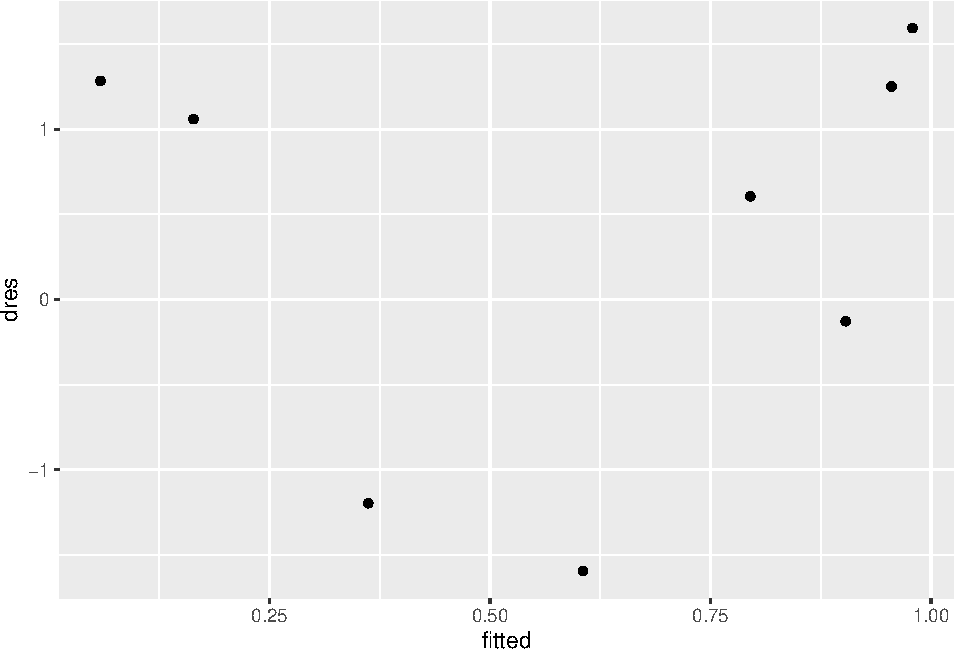
\includegraphics{3BinReg_files/figure-latex/unnamed-chunk-28-1.pdf}

\begin{Shaded}
\begin{Highlighting}[]
\FunctionTok{ggplot}\NormalTok{(df,}\FunctionTok{aes}\NormalTok{(}\AttributeTok{x=}\NormalTok{ldose,}\AttributeTok{y=}\NormalTok{dres))}\SpecialCharTok{+}\FunctionTok{geom\_point}\NormalTok{()}
\end{Highlighting}
\end{Shaded}

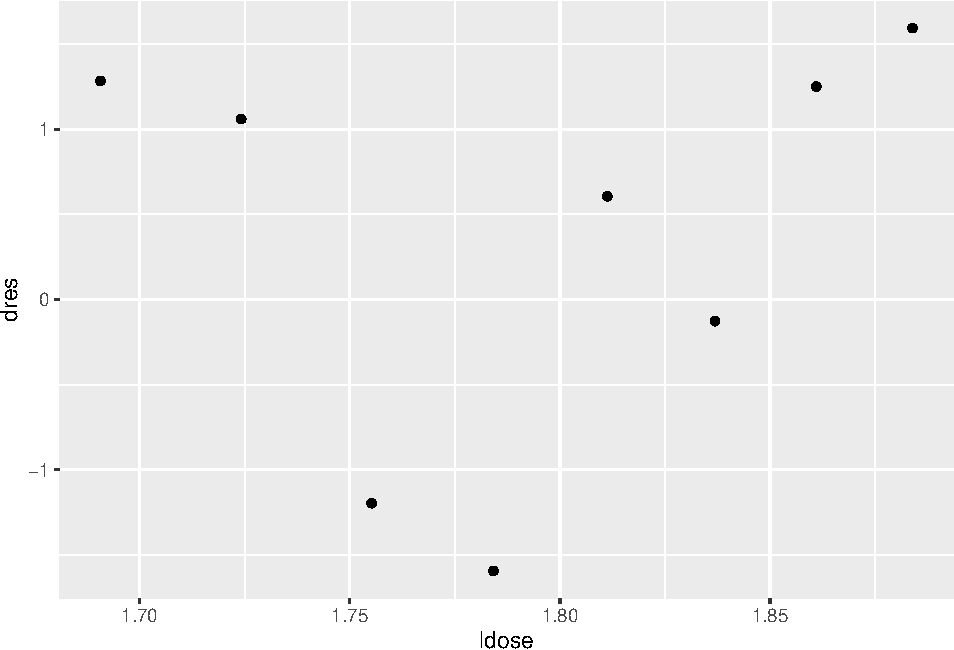
\includegraphics{3BinReg_files/figure-latex/unnamed-chunk-28-2.pdf}

\begin{center}\rule{0.5\linewidth}{0.5pt}\end{center}

\hypertarget{other-plots}{%
\subsection{Other plots}\label{other-plots}}

A useful plot is to show observed and fitted proportions (grouped data)
plotted against the linear predictor or covariates.

\begin{Shaded}
\begin{Highlighting}[]
\NormalTok{df}\OtherTok{=}\FunctionTok{data.frame}\NormalTok{(}\StringTok{"fitted"}\OtherTok{=}\NormalTok{fitgrouped}\SpecialCharTok{$}\NormalTok{fitted.values,}\StringTok{"dres"}\OtherTok{=}\FunctionTok{residuals}\NormalTok{(fitgrouped,}\AttributeTok{type=}\StringTok{"deviance"}\NormalTok{),}\StringTok{"ldose"}\OtherTok{=}\NormalTok{investr}\SpecialCharTok{::}\NormalTok{beetle}\SpecialCharTok{$}\NormalTok{ldose,}\StringTok{"frac"}\OtherTok{=}\NormalTok{investr}\SpecialCharTok{::}\NormalTok{beetle}\SpecialCharTok{$}\NormalTok{y}\SpecialCharTok{/}\NormalTok{investr}\SpecialCharTok{::}\NormalTok{beetle}\SpecialCharTok{$}\NormalTok{n)}
\FunctionTok{ggplot}\NormalTok{(df,}\FunctionTok{aes}\NormalTok{(}\AttributeTok{x=}\NormalTok{ldose))}\SpecialCharTok{+}\FunctionTok{geom\_point}\NormalTok{(}\FunctionTok{aes}\NormalTok{(}\AttributeTok{y=}\NormalTok{frac,}\AttributeTok{colour=}\StringTok{"observed"}\NormalTok{))}\SpecialCharTok{+}\FunctionTok{geom\_point}\NormalTok{(}\FunctionTok{aes}\NormalTok{(}\AttributeTok{y=}\NormalTok{fitted,}\AttributeTok{colour=}\StringTok{"fitted"}\NormalTok{))}
\end{Highlighting}
\end{Shaded}

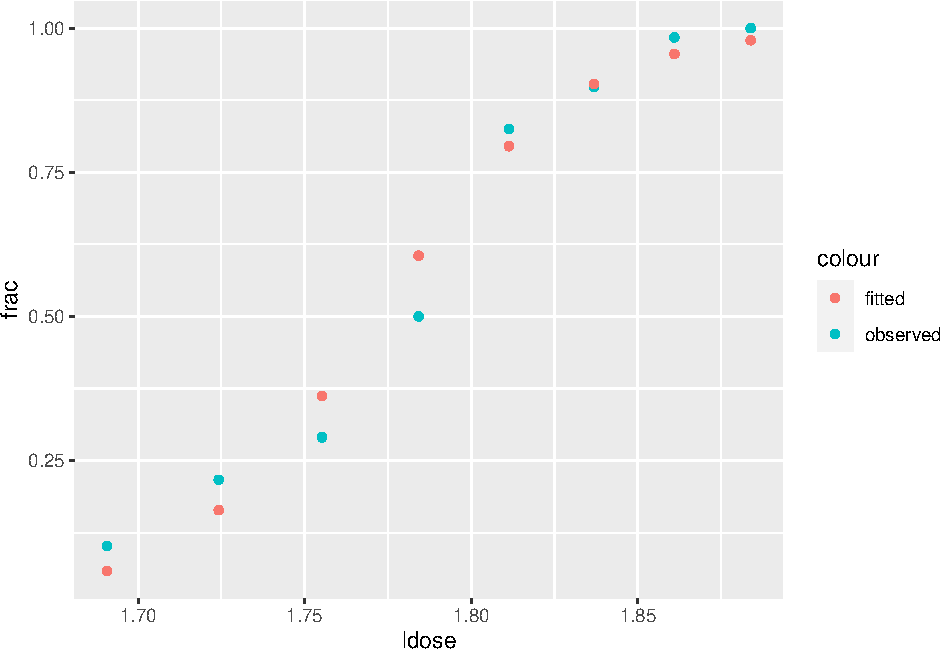
\includegraphics{3BinReg_files/figure-latex/unnamed-chunk-29-1.pdf}

\begin{center}\rule{0.5\linewidth}{0.5pt}\end{center}

\hypertarget{aic}{%
\subsection{AIC}\label{aic}}

It is known to us from multiple linear regression that if a model is
chosen based on a goodness of fit statistic (like the SSE or \(R^2\) in
multiple linear regression) will in general result in us choosing a to
big model (to many parameters fit). The Akaike informations criterion -
that we studied for multiple linear regression - can also be used for
binary regression: Let \(p\) be the number of regression parameters in
our model. \[\text{AIC} =-2 \cdot l(\hat{\boldsymbol{\beta}})+2p\] A
scaled version of AIC, standardizing for sample size, is sometimes
preferred.

To use AIC for model selection you use the model with the
\emph{smallest} AIC.

We may also use the BIC, where \(2p\) is replaced by \(\log(G)\cdot p\)
or \(\log(n)\cdot p\).

\begin{center}\rule{0.5\linewidth}{0.5pt}\end{center}

\footnotesize

\begin{Shaded}
\begin{Highlighting}[]
\FunctionTok{library}\NormalTok{(faraway)}
\NormalTok{fit1}\OtherTok{=}\FunctionTok{glm}\NormalTok{(}\FunctionTok{cbind}\NormalTok{(disease, nondisease)}\SpecialCharTok{\textasciitilde{}}\DecValTok{1}\NormalTok{,}\AttributeTok{family=}\FunctionTok{binomial}\NormalTok{(}\AttributeTok{link=}\NormalTok{logit),}\AttributeTok{data=}\NormalTok{babyfood)}
\NormalTok{fit2}\OtherTok{=}\FunctionTok{glm}\NormalTok{(}\FunctionTok{cbind}\NormalTok{(disease, nondisease)}\SpecialCharTok{\textasciitilde{}}\NormalTok{sex,}\AttributeTok{family=}\FunctionTok{binomial}\NormalTok{(}\AttributeTok{link=}\NormalTok{logit),}\AttributeTok{data=}\NormalTok{babyfood)}
\NormalTok{fit3}\OtherTok{=}\FunctionTok{glm}\NormalTok{(}\FunctionTok{cbind}\NormalTok{(disease, nondisease)}\SpecialCharTok{\textasciitilde{}}\NormalTok{food,}\AttributeTok{family=}\FunctionTok{binomial}\NormalTok{(}\AttributeTok{link=}\NormalTok{logit),}\AttributeTok{data=}\NormalTok{babyfood)}
\NormalTok{fit4}\OtherTok{=}\FunctionTok{glm}\NormalTok{(}\FunctionTok{cbind}\NormalTok{(disease, nondisease)}\SpecialCharTok{\textasciitilde{}}\NormalTok{food}\SpecialCharTok{+}\NormalTok{sex,}\AttributeTok{family=}\FunctionTok{binomial}\NormalTok{(}\AttributeTok{link=}\NormalTok{logit),}\AttributeTok{data=}\NormalTok{babyfood)}
\NormalTok{fit5}\OtherTok{=}\FunctionTok{glm}\NormalTok{(}\FunctionTok{cbind}\NormalTok{(disease, nondisease)}\SpecialCharTok{\textasciitilde{}}\NormalTok{food}\SpecialCharTok{*}\NormalTok{sex,}\AttributeTok{family=}\FunctionTok{binomial}\NormalTok{(}\AttributeTok{link=}\NormalTok{logit),}\AttributeTok{data=}\NormalTok{babyfood)}
\FunctionTok{AIC}\NormalTok{(fit1,fit2,fit3,fit4,fit5)}
\end{Highlighting}
\end{Shaded}

\begin{verbatim}
##      df      AIC
## fit1  1 59.89324
## fit2  2 56.41710
## fit3  3 43.21693
## fit4  4 40.23987
## fit5  6 43.51795
\end{verbatim}

\normalsize

\textbf{Q}: Which of these 5 models would you prefer?

\hypertarget{overdispersion-and-estimating-overdispersion-parameter}{%
\section{Overdispersion and estimating overdispersion
parameter}\label{overdispersion-and-estimating-overdispersion-parameter}}

When we have grouped data: \(Y_j \sim \text{Bin} (n_j, \pi_j)\) and
Var\((Y_j) = n_j\pi_j(1-\pi_j)\).

It is possible to estimate the variance (within a group) by
\(n_j\bar{y_j}(1-\bar{y_j})\) where \(\bar{y_j} = y_j/n_j\) (this is an
estimate of \(\pi_j\) for group \(j\)). We call this the \emph{empirical
variance}.

In a logistic regresson we estimate
\(\hat{\pi}_j = h({\bf x}_j^T\hat{\boldsymbol{\beta}})\) (\(h(\cdot)\)
is the inverse link function) which is

\[\hat{\pi_j} = \frac{\exp(x_j^T \hat{\boldsymbol{\beta}})}{1+\exp(x_j^T \hat{\boldsymbol{\beta}})} \]

for a logistic regression. This would give the \emph{estimated binomial
variance} for \(Y_j\) as \(n_j\hat{\pi_j}(1-\hat{\pi_j})\).

\begin{center}\rule{0.5\linewidth}{0.5pt}\end{center}

Some times the empirical variance is much larger than the estimated
binomial variance of the model. This is called \emph{overdispersion} and
may occur when the individual responses within the groups are
correlated, or when the model could be improved upon (missing/unobserved
covariates?).

Positively correlated binary variables will give a variance of the sum
that is larger than for uncorrelated variables, e.g.

\[\text{Var}(\sum_{k=1}^K Y_k) = \sum_{k=1}^K\text{Var}(Y_k) + 2\sum_{k<l} \text{Cov}(Y_k, Y_l).\]

\begin{center}\rule{0.5\linewidth}{0.5pt}\end{center}

This can be handeled by including an \emph{overdispersion parameter},
named \(\phi\), in the variance formula:

\[ \text{Var}(Y_j) = \phi n_j \pi_j (1-\pi_j)\]

\begin{center}\rule{0.5\linewidth}{0.5pt}\end{center}

The overdispersion parameter can be estimated as the average Pearson
statistic or average deviance

\[\hat{\phi}_D = \frac{1}{G-p} D\]

where \(D\) is the deviance. Note that similarity to
\(\hat{\sigma^2} = 1/(n-p)\cdot\text{SSE}\) in the MLR. The
Cov\((\hat{\boldsymbol{\beta}})\) can then be changed to
\(\hat{\phi}F^{-1}(\hat{\boldsymbol{\beta}})\).

Remark: We are now moving from likelihood to quasi-likelihood theory,
where only E\((Y_j)\) and Var\((Y_j)\) - and not the distribution of
\(Y_j\) - are used in the estimation.

In Modules 7 and 8 we will look at using multilevel models to handle
correlated observations.

\begin{center}\rule{0.5\linewidth}{0.5pt}\end{center}

\begin{Shaded}
\begin{Highlighting}[]
\FunctionTok{library}\NormalTok{(investr)}
\NormalTok{estpi}\OtherTok{=}\NormalTok{investr}\SpecialCharTok{::}\NormalTok{beetle}\SpecialCharTok{$}\NormalTok{y}\SpecialCharTok{/}\NormalTok{investr}\SpecialCharTok{::}\NormalTok{beetle}\SpecialCharTok{$}\NormalTok{n}
\NormalTok{empvars}\OtherTok{=}\NormalTok{investr}\SpecialCharTok{::}\NormalTok{beetle}\SpecialCharTok{$}\NormalTok{n}\SpecialCharTok{*}\NormalTok{estpi}\SpecialCharTok{*}\NormalTok{(}\DecValTok{1}\SpecialCharTok{{-}}\NormalTok{estpi)}
\NormalTok{fit}\OtherTok{=}\FunctionTok{glm}\NormalTok{(}\FunctionTok{cbind}\NormalTok{(y, n}\SpecialCharTok{{-}}\NormalTok{y) }\SpecialCharTok{\textasciitilde{}}\NormalTok{ ldose, }\AttributeTok{family =} \StringTok{"binomial"}\NormalTok{, }\AttributeTok{data =}\NormalTok{ investr}\SpecialCharTok{::}\NormalTok{beetle)}
\NormalTok{modelestvar}\OtherTok{=}\NormalTok{investr}\SpecialCharTok{::}\NormalTok{beetle}\SpecialCharTok{$}\NormalTok{n}\SpecialCharTok{*}\NormalTok{fit}\SpecialCharTok{$}\NormalTok{fitted.values}\SpecialCharTok{*}\NormalTok{(}\DecValTok{1}\SpecialCharTok{{-}}\NormalTok{fit}\SpecialCharTok{$}\NormalTok{fitted.values)}
\FunctionTok{cbind}\NormalTok{(empvars,modelestvar)}
\end{Highlighting}
\end{Shaded}

\begin{verbatim}
##     empvars modelestvar
## 1  5.389831    3.254850
## 2 10.183333    8.227364
## 3 12.774194   14.321308
## 4 14.000000   13.378891
## 5  9.079365   10.261038
## 6  5.389831    5.156652
## 7  0.983871    2.653383
## 8  0.000000    1.230704
\end{verbatim}

\begin{Shaded}
\begin{Highlighting}[]
\NormalTok{est.dispersion}\OtherTok{=}\NormalTok{fit}\SpecialCharTok{$}\NormalTok{deviance}\SpecialCharTok{/}\NormalTok{fit}\SpecialCharTok{$}\NormalTok{df.residual }
\NormalTok{est.dispersion}
\end{Highlighting}
\end{Shaded}

\begin{verbatim}
## [1] 1.872039
\end{verbatim}

\begin{Shaded}
\begin{Highlighting}[]
\FunctionTok{summary}\NormalTok{(fit,}\AttributeTok{dispersion=}\NormalTok{est.dispersion,}\AttributeTok{correlation=}\ConstantTok{TRUE}\NormalTok{)}
\end{Highlighting}
\end{Shaded}

\begin{verbatim}
## 
## Call:
## glm(formula = cbind(y, n - y) ~ ldose, family = "binomial", data = investr::beetle)
## 
## Coefficients:
##             Estimate Std. Error z value Pr(>|z|)    
## (Intercept)  -60.717      7.088  -8.566   <2e-16 ***
## ldose         34.270      3.984   8.601   <2e-16 ***
## ---
## Signif. codes:  0 '***' 0.001 '**' 0.01 '*' 0.05 '.' 0.1 ' ' 1
## 
## (Dispersion parameter for binomial family taken to be 1.872039)
## 
##     Null deviance: 284.202  on 7  degrees of freedom
## Residual deviance:  11.232  on 6  degrees of freedom
## AIC: 41.43
## 
## Number of Fisher Scoring iterations: 4
## 
## Correlation of Coefficients:
##       (Intercept)
## ldose -1.00
\end{verbatim}

\begin{Shaded}
\begin{Highlighting}[]
\NormalTok{fitquasi}\OtherTok{=}\FunctionTok{glm}\NormalTok{(}\FunctionTok{cbind}\NormalTok{(y, n}\SpecialCharTok{{-}}\NormalTok{y) }\SpecialCharTok{\textasciitilde{}}\NormalTok{ ldose, }\AttributeTok{family =} \StringTok{"quasibinomial"}\NormalTok{, }\AttributeTok{data =}\NormalTok{ investr}\SpecialCharTok{::}\NormalTok{beetle)}
\CommentTok{\# preferred method of estimation is to use quasilikelihood}
\FunctionTok{summary}\NormalTok{(fitquasi)}\SpecialCharTok{$}\NormalTok{dispersion}
\end{Highlighting}
\end{Shaded}

\begin{verbatim}
## [1] 1.671141
\end{verbatim}

\hypertarget{prospective-vs.-retrospective-sampling}{%
\section{Prospective vs.~retrospective
sampling}\label{prospective-vs.-retrospective-sampling}}

This section is optional - but it is very useful if you will work within
biostatistics. (Examples motivated by Faraway (2006), Extending the
linear model with R, Section 2.6.)

In a \emph{prospective sampling} strategy we sample individuals from a
population (covariates are then fixed) and wait for a predefined period
to check if an event has happend (e.g.~disease). This is also called a
\emph{cohort study}. An example might be that we select a sample of
newborn babies (girls and boys) where the parents had decided on the
method of feeding (bottle, breast, breast with some supplement), and
then monitored the babies during their first year to see if they
developed infant respiratory disease (the event we want to model). For
rare events the sample may then include few individuals with success
(disease), which might lead to wide confidence intervals for parameters.

An alternative strategy is called \emph{retrospective sampling}. Here we
have access to medical registers and select a sample of \(n_1\) babies
where we know that they developed infant respiratory disease (the
\emph{cases}) and a sample of \(n_2\) babies where we know that they did
not develop infant respiratory disease (the \emph{controls}). We require
that the samples are selected independently of the values of the
covariates (here: sex and food=method of feeding). This is called a
\emph{case--control study}.

If we aim to \emph{model the relationship between the covariates and the
response} (here: infant respiratory disease) we would naturally by
default choose the cohort design, however, we will now show that the
case--control design is also a valid design \emph{if} we use the logit
model to analyse the data.

To illustrate this we use a data set from a prospective study,

\begin{Shaded}
\begin{Highlighting}[]
\FunctionTok{library}\NormalTok{(faraway)}
\FunctionTok{data}\NormalTok{(babyfood)}
\FunctionTok{head}\NormalTok{(babyfood)}
\end{Highlighting}
\end{Shaded}

\begin{verbatim}
##   disease nondisease  sex   food
## 1      77        381  Boy Bottle
## 2      19        128  Boy  Suppl
## 3      47        447  Boy Breast
## 4      48        336 Girl Bottle
## 5      16        111 Girl  Suppl
## 6      31        433 Girl Breast
\end{verbatim}

\begin{Shaded}
\begin{Highlighting}[]
\FunctionTok{xtabs}\NormalTok{(disease}\SpecialCharTok{/}\NormalTok{(disease}\SpecialCharTok{+}\NormalTok{nondisease)}\SpecialCharTok{\textasciitilde{}}\NormalTok{sex}\SpecialCharTok{+}\NormalTok{food,babyfood)}
\end{Highlighting}
\end{Shaded}

\begin{verbatim}
##       food
## sex        Bottle     Breast      Suppl
##   Boy  0.16812227 0.09514170 0.12925170
##   Girl 0.12500000 0.06681034 0.12598425
\end{verbatim}

and for simplicity we focus on girls who were breast or bottle fed:

\begin{Shaded}
\begin{Highlighting}[]
\NormalTok{babyfood[}\FunctionTok{c}\NormalTok{(}\DecValTok{4}\NormalTok{,}\DecValTok{6}\NormalTok{),]}
\end{Highlighting}
\end{Shaded}

\begin{verbatim}
##   disease nondisease  sex   food
## 4      48        336 Girl Bottle
## 6      31        433 Girl Breast
\end{verbatim}

Notice - we now look at the observed data within the different covariate
patterns. This would be the same as fitting a binomial glm with sex,
food and the interaction thereof as covariates.

We read off: given that the infant is breast fed: 31/433= 0.07 is the
estimated odds of respiratory disease, and the log-odds is -2.64. And,
given that the infant is bottle fed: 48/336= 0.14 is the estimated odds
of respiratory disease, and the log-odds is -1.95. The difference
between these two log-odds represents the increased risk of infant
respiratory disease caused by bottle feeding relative to breast feeding:

\(\Delta\)= -1.95- -2.64= 0.69.

But, what if we instead had performed a case--control study, and then
wanted to compute the log odds difference between feeding type given
respiratory disease status.

We read off: given that the infant got the disease (case): 48/31= 1.55
is the estimated odds for bottle compared to breast, and the log-odds is
0.44. Given that the infant did not get the disease (control): 336/433=
0.78 is the estimated odds for bottle compared to breast, and the
log-odds is -0.25. The difference between these two log-odds represents
the ``increased risk'' of bottle feeding relative to breast feeding
``caused by respiratory disease''.

\(\Delta^*\)=0.44- -0.25=0.69.

Observe that \(\Delta\) and \(\Delta^*\) are equal, and shows (with a
numerical example) why a retrospective design can be use to estimate
change in log-odds. But, this argumentation is only valid for our logit
model (where we estimate changes in odds), and not for the probit or
complementary-log-log model.

We would like to use the retrospective case--control design instead of
the prospective cohort design because it is more convenient to get a
sample of cases on the same size as a sample of controls - which give us
better properties of the parameter estimators. However, to use the
case--control design it is important that covariates are reliably
measured retrospective (rely on records).

In a mathematical comparison between logit models for pro- and
retrospective designs we will find that the regression parameters
\(\beta_1, \ldots, \beta_k\) will be the same in the two models, but the
intercept terms will differ.

In the prospectictive study we model \(\pi_i\), the probability of
sucess (e.g.~respiratory disease) for covariates
\(x_{i1}, x_{i2}, \ldots, x_{ik}\) (e.g.~sex and food). Using the logit
model in the proseptive study, the regression model is
\[ \ln (\frac{\pi_i}{1-\pi_i}) = \eta_i =  \beta_0+\beta_1 x_{i1}+\beta_2 x_{i2}+\cdots + \beta_k x_{ik} \]
and we write \[ \pi_i=\frac{\exp(\eta_i)}{1+\exp(\eta_i)}.\]

In a retrospective study we consider \(\rho_i\), the probability of
sucess for covariates \(x_{i1}, x_{i2}, \ldots, x_{ik}\), given that
individual \(i\) was sampled to be part of the case-control study.

Let \(S\) denote the event `sampled', and let \(D\) denote event
`disease' (or sucess). Then, using Bayes' rule and the law of total
probability, we have
\[ \rho_i= P_i(D|S) = \frac{P_i(D \cap S)}{P_i(S)} = \frac{P_i(S|D)P_i(D)}{P_i(S|D)P_i(D) + P_i(S|D^c)P_i(D^c)}  \]
where \(P_i(D) = \pi_i\) and \(P_i(D^c) = 1-\pi_i\).

In the retrospective study, the probability of being sampled is equal
for any individual with the disease; \(\tau_1 = P(S|D) = P_i(S|D)\) and
similarly for individuals who do not have the disease;
\(\tau_0 = P(S|D^c) = P_i(S|D^c)\). Then,
\[ \rho_i= \frac{\tau_1 \pi_i}{\tau_1 \pi_i + \tau_0 (1-\pi_i)}  =  \frac{\tau_1 \frac{\exp(\eta_i)}{1+\exp(\eta_i)}}{\tau_1 \frac{\exp(\eta_i)}{1+\exp(\eta_i)} + \tau_0 \frac{1}{1+\exp(\eta_i)}}\]

Dividing by \(\tau_0\) and multiplying by \(1+\exp(\eta_i)\) in the
numerator and denominator gives
\[ \rho_i= \frac{(\tau_1/\tau_0) \exp(\eta_i)}{(\tau_1/\tau_0) \exp(\eta_i) + 1} = \frac{\exp(\ln(\tau_1/\tau_0) + \eta_i)}{\exp(\ln(\tau_1/\tau_0) + \eta_i) + 1}\]

Using the logit model for \(\rho_i\) in the retrospective model, the
regression model is
\[ \ln (\frac{\rho_i}{1-\rho_i}) = \ln(\tau_1/\tau_0) + \eta_i = \ln(\tau_1/\tau_0) + \beta_0+\beta_1 x_{i1}+\beta_2 x_{i2}+\cdots + \beta_k x_{ik} \]
We see that the only difference between the parameters of interest in
the retrospective study and the parameters of interest in the
prospective study is the intercept of the regression model. All other
covariates are equal.

\hypertarget{interactive-lecture---second-week}{%
\section{Interactive lecture - second
week}\label{interactive-lecture---second-week}}

We will use a data set on contraceptive use in Fiji (data from 1975).
The data is to be analysed with ``current use of contraceptive'' as
response and some (or all of) ``age'', ``level of education'', ``desire
for more children'' as covariates

The data is available at
\url{https://grodri.github.io/datasets/cuse.dat} with the following
description:

\begin{itemize}
\tightlist
\item
  Contraceptive use: yes (\texttt{using}) or no (\texttt{notUsing})
\item
  \texttt{age}: categorical variable with 5 levels: ``\textless25'',
  ``25-29'', ``30-39'', ``40-49''
\item
  \texttt{education}: categorical variable with 2 levels giving highest
  level of education obtained: Lower and Upper
\item
  \texttt{wantsMore}: Desires more children: yes or no
\end{itemize}

\begin{Shaded}
\begin{Highlighting}[]
\NormalTok{ds}\OtherTok{=}\FunctionTok{read.table}\NormalTok{(}\StringTok{"https://grodri.github.io/datasets/cuse.dat"}\NormalTok{,}\AttributeTok{header=}\ConstantTok{TRUE}\NormalTok{)}
\FunctionTok{names}\NormalTok{(ds)}
\end{Highlighting}
\end{Shaded}

\begin{verbatim}
## [1] "age"       "education" "wantsMore" "notUsing"  "using"
\end{verbatim}

\begin{Shaded}
\begin{Highlighting}[]
\FunctionTok{summary}\NormalTok{(ds)}
\end{Highlighting}
\end{Shaded}

\begin{verbatim}
##      age             education          wantsMore            notUsing     
##  Length:16          Length:16          Length:16          Min.   :  8.00  
##  Class :character   Class :character   Class :character   1st Qu.: 31.00  
##  Mode  :character   Mode  :character   Mode  :character   Median : 56.50  
##                                                           Mean   : 68.75  
##                                                           3rd Qu.: 85.75  
##                                                           Max.   :212.00  
##      using      
##  Min.   : 4.00  
##  1st Qu.: 9.50  
##  Median :29.00  
##  Mean   :31.69  
##  3rd Qu.:49.00  
##  Max.   :80.00
\end{verbatim}

\begin{Shaded}
\begin{Highlighting}[]
\FunctionTok{dim}\NormalTok{(ds)}
\end{Highlighting}
\end{Shaded}

\begin{verbatim}
## [1] 16  5
\end{verbatim}

\begin{Shaded}
\begin{Highlighting}[]
\FunctionTok{head}\NormalTok{(ds)}
\end{Highlighting}
\end{Shaded}

\begin{verbatim}
##     age education wantsMore notUsing using
## 1   <25       low       yes       53     6
## 2   <25       low        no       10     4
## 3   <25      high       yes      212    52
## 4   <25      high        no       50    10
## 5 25-29       low       yes       60    14
## 6 25-29       low        no       19    10
\end{verbatim}

We will study binary regression using the logit model, and we will work
with grouped data.

\textbf{Plan: Start with Problem 2, then move to 3 and 4, and if you
have time you look at Problem 1. We will do a team Kahoot! in the end of
the IL - on one device go to kahoot.it or use an app version. }

\hypertarget{problem-1-the-null-model---no-covariates-included.}{%
\subsubsection{Problem 1: The null model - no covariates
included.}\label{problem-1-the-null-model---no-covariates-included.}}

(This is the most theoretical of the problems and rather technical - but
with some cool results on the null model.)

\textbf{a)} Fit the null model and call it \texttt{fit0}. Explain what
you see.

\begin{Shaded}
\begin{Highlighting}[]
\NormalTok{fit0}\OtherTok{=}\FunctionTok{glm}\NormalTok{(}\FunctionTok{cbind}\NormalTok{(using,notUsing)}\SpecialCharTok{\textasciitilde{}}\DecValTok{1}\NormalTok{,}\AttributeTok{data=}\NormalTok{ds,}\AttributeTok{family=}\FunctionTok{binomial}\NormalTok{(}\AttributeTok{link=}\NormalTok{logit))}
\FunctionTok{summary}\NormalTok{(fit0)}
\end{Highlighting}
\end{Shaded}

\begin{verbatim}
## 
## Call:
## glm(formula = cbind(using, notUsing) ~ 1, family = binomial(link = logit), 
##     data = ds)
## 
## Coefficients:
##             Estimate Std. Error z value Pr(>|z|)    
## (Intercept) -0.77455    0.05368  -14.43   <2e-16 ***
## ---
## Signif. codes:  0 '***' 0.001 '**' 0.01 '*' 0.05 '.' 0.1 ' ' 1
## 
## (Dispersion parameter for binomial family taken to be 1)
## 
##     Null deviance: 165.77  on 15  degrees of freedom
## Residual deviance: 165.77  on 15  degrees of freedom
## AIC: 239.28
## 
## Number of Fisher Scoring iterations: 4
\end{verbatim}

Observe: When we only have an intercept in the model, the model matrix
will be an \(n \times 1\)-matrix with only ones. Then
\({\bf x}_j^T\boldsymbol{\beta}=\beta_0\). The log-likelihood can be
written as (let \(j=1,\ldots,G\))

\begin{align} l(\boldsymbol{\beta}) &=\sum_{j=1}^G (y_j{\bf x}_j^T \boldsymbol{\beta} - n_j \log(1+\exp({\bf x}_j^T\boldsymbol{\beta})))= \sum_{j=1}^G (y_j\beta_0 - n_j \log(1+\exp(\beta_0)))\\
&= \beta_0 \sum_{j=1}^G y_j - \log(1+\exp(\beta_0))\sum_{j=1}^G n_j =\beta_0 N_1 - \log(1+\exp(\beta_0))N
\end{align} where \(N_1=\sum_{j=1}^G y_j\) is the total number of
successes and \(N=\sum_{j=1}^G n_j\) is the total number of trials (over
all covariates patterns, that is, here the number of individuals in the
data set). Also \(N_2=N-N_1\) is the total number of failures.

We will use this loglikelihood in the next question.

\textbf{b)} What is the relationship between your estimated coefficient
and the proportion in the data set using contraception (\(N_1/N\))?
(Hint 0: What would be your intuitive estimator for \(\pi\) (common to
all groups). Hint 1: Find the derivative of the log-likelihood with
respect to \(\beta_0\), and use this to find the MLE for \(\beta_0\).
Hint 2: maybe easier to see what \(\hat{\pi}\) is, where
\(\hat{\pi}=\frac{\exp{\hat{\beta}_0}}{1+\exp{\hat{\beta}_0}}\) (so
\texttt{plogis}), and then
\(\hat{\boldsymbol{\beta}}_0=\text{logit}(\hat{\pi})\) (so
\texttt{qlogis}). Hint 3: You can verify by using the estimate from
\texttt{glm}.)

\begin{Shaded}
\begin{Highlighting}[]
\NormalTok{N }\OtherTok{=} \FunctionTok{sum}\NormalTok{(ds}\SpecialCharTok{$}\NormalTok{using }\SpecialCharTok{+}\NormalTok{ ds}\SpecialCharTok{$}\NormalTok{notUsing)}
\NormalTok{N}
\end{Highlighting}
\end{Shaded}

\begin{verbatim}
## [1] 1607
\end{verbatim}

\begin{Shaded}
\begin{Highlighting}[]
\NormalTok{N1 }\OtherTok{=} \FunctionTok{sum}\NormalTok{(ds}\SpecialCharTok{$}\NormalTok{using)}
\NormalTok{N1}
\end{Highlighting}
\end{Shaded}

\begin{verbatim}
## [1] 507
\end{verbatim}

\begin{Shaded}
\begin{Highlighting}[]
\NormalTok{N2 }\OtherTok{=}\NormalTok{ N }\SpecialCharTok{{-}}\NormalTok{ N1}
\NormalTok{N2}
\end{Highlighting}
\end{Shaded}

\begin{verbatim}
## [1] 1100
\end{verbatim}

\begin{Shaded}
\begin{Highlighting}[]
\FunctionTok{qlogis}\NormalTok{(N1}\SpecialCharTok{/}\NormalTok{N)}
\end{Highlighting}
\end{Shaded}

\begin{verbatim}
## [1] -0.7745545
\end{verbatim}

\begin{Shaded}
\begin{Highlighting}[]
\NormalTok{fit0}\SpecialCharTok{$}\NormalTok{coefficients}
\end{Highlighting}
\end{Shaded}

\begin{verbatim}
## (Intercept) 
##  -0.7745545
\end{verbatim}

\textbf{c)} We know that the (asymptotic) estimated covariance matrix of
the ML estimate is the inverse of the expected Fisher information
matrix, here the matrix is only a scalar and the covariance matrix is
just the variance. Find the mathematical expression for the estimated
variance of our estimated intercept. (Hint 1: We have
\(F(\boldsymbol{\beta}) = \sum_{j=1}^G x_jx_j^T n_j \pi_j(1-\pi_j)\),
and then insert \(x_j = 1\) and \(\pi_j(1-\pi_j)=\pi(1-\pi)\), and
hopefully you found above that \(\hat{\pi}=N_1/N\) in our model with
only intercept. Hint 2:
\(\frac{N}{N_1 \cdot N_2}=\frac{1}{N_1}+\frac{1}{N_2}\) to make things
prettier.)

\textbf{d)} What is the estimated (numerical value) standard deviation
of the parameter estimate? Hint: \texttt{vcov(fit0)}. Did your
calculation above gives the same result?

\begin{Shaded}
\begin{Highlighting}[]
\FunctionTok{vcov}\NormalTok{(fit0)}
\end{Highlighting}
\end{Shaded}

\begin{verbatim}
##             (Intercept)
## (Intercept) 0.002881477
\end{verbatim}

\textbf{e)} What is the asymptotic distribution of the estimated
regression coefficient? Use this to write down the formula for the 95\%
confidence interval for the intercept, and calculate the interval in R.
Compare numerically to \texttt{confint.default} and \texttt{confint}.

\begin{Shaded}
\begin{Highlighting}[]
\NormalTok{ci}\OtherTok{=}\FunctionTok{confint.default}\NormalTok{(fit0)}
\NormalTok{ci}
\end{Highlighting}
\end{Shaded}

\begin{verbatim}
##                  2.5 %     97.5 %
## (Intercept) -0.8797641 -0.6693448
\end{verbatim}

\begin{Shaded}
\begin{Highlighting}[]
\FunctionTok{confint}\NormalTok{(fit0)}
\end{Highlighting}
\end{Shaded}

\begin{verbatim}
##      2.5 %     97.5 % 
## -0.8804716 -0.6700014
\end{verbatim}

\textbf{f)} Translate the 95\% CI to probability scale (Hint:
\texttt{plogis} is the inverse logit.)

\begin{Shaded}
\begin{Highlighting}[]
\FunctionTok{plogis}\NormalTok{(ci)}
\end{Highlighting}
\end{Shaded}

\begin{verbatim}
##                 2.5 %    97.5 %
## (Intercept) 0.2932267 0.3386436
\end{verbatim}

\begin{Shaded}
\begin{Highlighting}[]
\NormalTok{fit0}\SpecialCharTok{$}\NormalTok{family}\SpecialCharTok{$}\FunctionTok{linkinv}\NormalTok{(ci)}
\end{Highlighting}
\end{Shaded}

\begin{verbatim}
##                 2.5 %    97.5 %
## (Intercept) 0.2932267 0.3386436
\end{verbatim}

\hypertarget{problem-2-we-then-study-the-effect-of-the-covariate-wantsmore}{%
\subsubsection{Problem 2: We then study the effect of the covariate
``wantsMore''}\label{problem-2-we-then-study-the-effect-of-the-covariate-wantsmore}}

(a little less maths)

\textbf{a)} Fit a regression with \texttt{wantsMore} as covariate, and
call this \texttt{fit1}. Explain what the estimated coefficient
(\(\beta_1\)) means. Hint: Interpretation using odds -- if `wantsMore´
goes from 0=no to 1=yes, then\ldots{}

\begin{Shaded}
\begin{Highlighting}[]
\NormalTok{fit1}\OtherTok{=}\FunctionTok{glm}\NormalTok{(}\FunctionTok{cbind}\NormalTok{(using,notUsing)}\SpecialCharTok{\textasciitilde{}}\NormalTok{wantsMore,}\AttributeTok{data=}\NormalTok{ds,}\AttributeTok{family=}\NormalTok{binomial)}
\FunctionTok{summary}\NormalTok{(fit1)}
\end{Highlighting}
\end{Shaded}

\begin{verbatim}
## 
## Call:
## glm(formula = cbind(using, notUsing) ~ wantsMore, family = binomial, 
##     data = ds)
## 
## Coefficients:
##              Estimate Std. Error z value Pr(>|z|)    
## (Intercept)  -0.18636    0.07971  -2.338   0.0194 *  
## wantsMoreyes -1.04863    0.11067  -9.475   <2e-16 ***
## ---
## Signif. codes:  0 '***' 0.001 '**' 0.01 '*' 0.05 '.' 0.1 ' ' 1
## 
## (Dispersion parameter for binomial family taken to be 1)
## 
##     Null deviance: 165.772  on 15  degrees of freedom
## Residual deviance:  74.098  on 14  degrees of freedom
## AIC: 149.61
## 
## Number of Fisher Scoring iterations: 4
\end{verbatim}

\begin{Shaded}
\begin{Highlighting}[]
\FunctionTok{exp}\NormalTok{(fit1}\SpecialCharTok{$}\NormalTok{coefficients)}
\end{Highlighting}
\end{Shaded}

\begin{verbatim}
##  (Intercept) wantsMoreyes 
##    0.8299712    0.3504178
\end{verbatim}

\textbf{b)} Is this covariate significant? Write down the null and
alternative hypothesis to test. Then test using the Wald test - write
down the formula yourself. Use \texttt{vcov(fit1)} to access the inverse
of the Fisher information matrix. What is the degrees of freedom for
this test? Compare to the print-out from \texttt{summary}.

\begin{Shaded}
\begin{Highlighting}[]
\FunctionTok{vcov}\NormalTok{(fit1)}
\end{Highlighting}
\end{Shaded}

\begin{verbatim}
##               (Intercept) wantsMoreyes
## (Intercept)   0.006354067 -0.006354067
## wantsMoreyes -0.006354067  0.012248298
\end{verbatim}

\textbf{c)} Alternatively, the likelihood ratio test can be used. Write
down the formula for the likelihood ratio test statistic. Use this in
combination with the \texttt{fit0} and \texttt{fit1} objects to
calculate the likelihood ratio statistic. Then calculate the
\(p\)-value.

\begin{Shaded}
\begin{Highlighting}[]
\NormalTok{loglik }\OtherTok{\textless{}{-}} \ControlFlowTok{function}\NormalTok{(par, args) \{}
\NormalTok{    y }\OtherTok{\textless{}{-}}\NormalTok{ args}\SpecialCharTok{$}\NormalTok{y}
\NormalTok{    x }\OtherTok{\textless{}{-}}\NormalTok{ args}\SpecialCharTok{$}\NormalTok{x}
\NormalTok{    n }\OtherTok{\textless{}{-}}\NormalTok{ args}\SpecialCharTok{$}\NormalTok{n}
\NormalTok{    res }\OtherTok{\textless{}{-}} \FunctionTok{sum}\NormalTok{(y }\SpecialCharTok{*}\NormalTok{ x }\SpecialCharTok{\%*\%}\NormalTok{ par }\SpecialCharTok{{-}}\NormalTok{ n }\SpecialCharTok{*} \FunctionTok{log}\NormalTok{(}\DecValTok{1} \SpecialCharTok{+} \FunctionTok{exp}\NormalTok{(x }\SpecialCharTok{\%*\%}\NormalTok{ par)))}
    \FunctionTok{return}\NormalTok{(res)}
\NormalTok{\}}

\NormalTok{args0 }\OtherTok{\textless{}{-}} \FunctionTok{list}\NormalTok{(}\AttributeTok{y =}\NormalTok{ ds}\SpecialCharTok{$}\NormalTok{using, }\AttributeTok{n =}\NormalTok{ ds}\SpecialCharTok{$}\NormalTok{using }\SpecialCharTok{+}\NormalTok{ ds}\SpecialCharTok{$}\NormalTok{notUsing, }\AttributeTok{x =} \FunctionTok{cbind}\NormalTok{(}\FunctionTok{rep}\NormalTok{(}\DecValTok{1}\NormalTok{, }\FunctionTok{nrow}\NormalTok{(ds))))}
\NormalTok{args1 }\OtherTok{\textless{}{-}} \FunctionTok{list}\NormalTok{(}\AttributeTok{y =}\NormalTok{ ds}\SpecialCharTok{$}\NormalTok{using, }\AttributeTok{n =}\NormalTok{ ds}\SpecialCharTok{$}\NormalTok{using }\SpecialCharTok{+}\NormalTok{ ds}\SpecialCharTok{$}\NormalTok{notUsing, }\AttributeTok{x =} \FunctionTok{cbind}\NormalTok{(}\FunctionTok{rep}\NormalTok{(}\DecValTok{1}\NormalTok{, }\FunctionTok{nrow}\NormalTok{(ds)), }
    \FunctionTok{as.numeric}\NormalTok{(ds}\SpecialCharTok{$}\NormalTok{wantsMore) }\SpecialCharTok{{-}} \DecValTok{1}\NormalTok{))}

\NormalTok{betas0 }\OtherTok{\textless{}{-}}\NormalTok{ fit0}\SpecialCharTok{$}\NormalTok{coefficients}
\NormalTok{betas1 }\OtherTok{\textless{}{-}}\NormalTok{ fit1}\SpecialCharTok{$}\NormalTok{coefficients}

\NormalTok{ll0 }\OtherTok{\textless{}{-}} \FunctionTok{loglik}\NormalTok{(betas0, args0)}
\NormalTok{ll0}
\end{Highlighting}
\end{Shaded}

\begin{verbatim}
## [1] -1001.847
\end{verbatim}

\begin{Shaded}
\begin{Highlighting}[]
\NormalTok{ll1 }\OtherTok{\textless{}{-}} \FunctionTok{loglik}\NormalTok{(betas1, args1)}
\NormalTok{ll1}
\end{Highlighting}
\end{Shaded}

\begin{verbatim}
## [1] NA
\end{verbatim}

\textbf{d)} The likelihood ratio test statistic can alternatively be
calculated using the residual deviance in \texttt{fit1} and
\texttt{fit0}, and is given as \texttt{fit0\$deviance-fit1\$deviance}.
Do you see why?

\begin{Shaded}
\begin{Highlighting}[]
\NormalTok{fit0}\SpecialCharTok{$}\NormalTok{deviance}\SpecialCharTok{{-}}\NormalTok{fit1}\SpecialCharTok{$}\NormalTok{deviance}
\end{Highlighting}
\end{Shaded}

\begin{verbatim}
## [1] 91.6744
\end{verbatim}

\textbf{e)} Are the two test statistics (Wald and LRT) equal? Do the two
tests give the same conclusions?

\hypertarget{problem-3-now-two-covariates---deviance-and-model-comparison}{%
\subsubsection{Problem 3: Now two covariates - deviance and model
comparison}\label{problem-3-now-two-covariates---deviance-and-model-comparison}}

(no maths - only definitions and print-out)

Now we study the response together with \texttt{age} and
\texttt{wantsMore}. We will consider the following 5 models. See R-code
and print-out below. \textbf{a)} Explain what each of these models
include.

\textbf{b)} What is the definition of the deviance and df. What can we
use the deviance for? Optional: derive the formula for the deviance for
the logit model (the derivation is not given on the module pages.)

\textbf{c)} Perform a likelihood ratio test - based on the deviance
results given in the data frame in the R chunk- to compare the additive
and interact models. First write down the null and alternative
hypothesis you are testing. Which of the two models would you prefer?

\textbf{d)} What if you use the AIC for model selection, which model
(out of the 5) will you then use?

\begin{Shaded}
\begin{Highlighting}[]
\NormalTok{ds}\SpecialCharTok{$}\NormalTok{Y }\OtherTok{\textless{}{-}} \FunctionTok{cbind}\NormalTok{(ds}\SpecialCharTok{$}\NormalTok{using, ds}\SpecialCharTok{$}\NormalTok{notUsing)}
\NormalTok{models }\OtherTok{\textless{}{-}} \FunctionTok{list}\NormalTok{(}
  \AttributeTok{null     =} \FunctionTok{glm}\NormalTok{(Y }\SpecialCharTok{\textasciitilde{}} \DecValTok{1}\NormalTok{, }\AttributeTok{family=}\NormalTok{binomial, }\AttributeTok{data=}\NormalTok{ds),}
  \AttributeTok{age      =} \FunctionTok{glm}\NormalTok{(Y }\SpecialCharTok{\textasciitilde{}}\NormalTok{ age, }\AttributeTok{family=}\NormalTok{binomial, }\AttributeTok{data=}\NormalTok{ds),}
  \AttributeTok{desire   =} \FunctionTok{glm}\NormalTok{(Y }\SpecialCharTok{\textasciitilde{}}\NormalTok{ wantsMore, }\AttributeTok{family=}\NormalTok{binomial, }\AttributeTok{data=}\NormalTok{ds),}
  \AttributeTok{additive =} \FunctionTok{glm}\NormalTok{(Y }\SpecialCharTok{\textasciitilde{}}\NormalTok{ age }\SpecialCharTok{+}\NormalTok{ wantsMore, }\AttributeTok{family=}\NormalTok{binomial, }\AttributeTok{data=}\NormalTok{ds),}
  \AttributeTok{interact =} \FunctionTok{glm}\NormalTok{(Y }\SpecialCharTok{\textasciitilde{}}\NormalTok{ age}\SpecialCharTok{*}\NormalTok{wantsMore, }\AttributeTok{family=}\NormalTok{binomial, }\AttributeTok{data=}\NormalTok{ds)}
\NormalTok{)}
\NormalTok{models}
\end{Highlighting}
\end{Shaded}

\begin{verbatim}
## $null
## 
## Call:  glm(formula = Y ~ 1, family = binomial, data = ds)
## 
## Coefficients:
## (Intercept)  
##     -0.7746  
## 
## Degrees of Freedom: 15 Total (i.e. Null);  15 Residual
## Null Deviance:       165.8 
## Residual Deviance: 165.8     AIC: 239.3
## 
## $age
## 
## Call:  glm(formula = Y ~ age, family = binomial, data = ds)
## 
## Coefficients:
## (Intercept)     age25-29     age30-39     age40-49  
##     -1.5072       0.4607       1.0483       1.4246  
## 
## Degrees of Freedom: 15 Total (i.e. Null);  12 Residual
## Null Deviance:       165.8 
## Residual Deviance: 86.58     AIC: 166.1
## 
## $desire
## 
## Call:  glm(formula = Y ~ wantsMore, family = binomial, data = ds)
## 
## Coefficients:
##  (Intercept)  wantsMoreyes  
##      -0.1864       -1.0486  
## 
## Degrees of Freedom: 15 Total (i.e. Null);  14 Residual
## Null Deviance:       165.8 
## Residual Deviance: 74.1  AIC: 149.6
## 
## $additive
## 
## Call:  glm(formula = Y ~ age + wantsMore, family = binomial, data = ds)
## 
## Coefficients:
##  (Intercept)      age25-29      age30-39      age40-49  wantsMoreyes  
##      -0.8698        0.3678        0.8078        1.0226       -0.8241  
## 
## Degrees of Freedom: 15 Total (i.e. Null);  11 Residual
## Null Deviance:       165.8 
## Residual Deviance: 36.89     AIC: 118.4
## 
## $interact
## 
## Call:  glm(formula = Y ~ age * wantsMore, family = binomial, data = ds)
## 
## Coefficients:
##           (Intercept)               age25-29               age30-39  
##               -1.4553                 0.6354                 1.5411  
##              age40-49           wantsMoreyes  age25-29:wantsMoreyes  
##                1.7643                -0.0640                -0.2672  
## age30-39:wantsMoreyes  age40-49:wantsMoreyes  
##               -1.0905                -1.3671  
## 
## Degrees of Freedom: 15 Total (i.e. Null);  8 Residual
## Null Deviance:       165.8 
## Residual Deviance: 20.1  AIC: 107.6
\end{verbatim}

\begin{Shaded}
\begin{Highlighting}[]
\FunctionTok{lapply}\NormalTok{(models,summary)}
\end{Highlighting}
\end{Shaded}

\begin{verbatim}
## $null
## 
## Call:
## glm(formula = Y ~ 1, family = binomial, data = ds)
## 
## Coefficients:
##             Estimate Std. Error z value Pr(>|z|)    
## (Intercept) -0.77455    0.05368  -14.43   <2e-16 ***
## ---
## Signif. codes:  0 '***' 0.001 '**' 0.01 '*' 0.05 '.' 0.1 ' ' 1
## 
## (Dispersion parameter for binomial family taken to be 1)
## 
##     Null deviance: 165.77  on 15  degrees of freedom
## Residual deviance: 165.77  on 15  degrees of freedom
## AIC: 239.28
## 
## Number of Fisher Scoring iterations: 4
## 
## 
## $age
## 
## Call:
## glm(formula = Y ~ age, family = binomial, data = ds)
## 
## Coefficients:
##             Estimate Std. Error z value Pr(>|z|)    
## (Intercept)  -1.5072     0.1303 -11.571  < 2e-16 ***
## age25-29      0.4607     0.1727   2.667  0.00765 ** 
## age30-39      1.0483     0.1544   6.788 1.14e-11 ***
## age40-49      1.4246     0.1940   7.345 2.06e-13 ***
## ---
## Signif. codes:  0 '***' 0.001 '**' 0.01 '*' 0.05 '.' 0.1 ' ' 1
## 
## (Dispersion parameter for binomial family taken to be 1)
## 
##     Null deviance: 165.772  on 15  degrees of freedom
## Residual deviance:  86.581  on 12  degrees of freedom
## AIC: 166.09
## 
## Number of Fisher Scoring iterations: 4
## 
## 
## $desire
## 
## Call:
## glm(formula = Y ~ wantsMore, family = binomial, data = ds)
## 
## Coefficients:
##              Estimate Std. Error z value Pr(>|z|)    
## (Intercept)  -0.18636    0.07971  -2.338   0.0194 *  
## wantsMoreyes -1.04863    0.11067  -9.475   <2e-16 ***
## ---
## Signif. codes:  0 '***' 0.001 '**' 0.01 '*' 0.05 '.' 0.1 ' ' 1
## 
## (Dispersion parameter for binomial family taken to be 1)
## 
##     Null deviance: 165.772  on 15  degrees of freedom
## Residual deviance:  74.098  on 14  degrees of freedom
## AIC: 149.61
## 
## Number of Fisher Scoring iterations: 4
## 
## 
## $additive
## 
## Call:
## glm(formula = Y ~ age + wantsMore, family = binomial, data = ds)
## 
## Coefficients:
##              Estimate Std. Error z value Pr(>|z|)    
## (Intercept)   -0.8698     0.1571  -5.536 3.10e-08 ***
## age25-29       0.3678     0.1754   2.097    0.036 *  
## age30-39       0.8078     0.1598   5.056 4.27e-07 ***
## age40-49       1.0226     0.2039   5.014 5.32e-07 ***
## wantsMoreyes  -0.8241     0.1171  -7.037 1.97e-12 ***
## ---
## Signif. codes:  0 '***' 0.001 '**' 0.01 '*' 0.05 '.' 0.1 ' ' 1
## 
## (Dispersion parameter for binomial family taken to be 1)
## 
##     Null deviance: 165.772  on 15  degrees of freedom
## Residual deviance:  36.888  on 11  degrees of freedom
## AIC: 118.4
## 
## Number of Fisher Scoring iterations: 4
## 
## 
## $interact
## 
## Call:
## glm(formula = Y ~ age * wantsMore, family = binomial, data = ds)
## 
## Coefficients:
##                       Estimate Std. Error z value Pr(>|z|)    
## (Intercept)            -1.4553     0.2968  -4.903 9.43e-07 ***
## age25-29                0.6354     0.3564   1.783  0.07463 .  
## age30-39                1.5412     0.3183   4.842 1.29e-06 ***
## age40-49                1.7643     0.3435   5.136 2.80e-07 ***
## wantsMoreyes           -0.0640     0.3303  -0.194  0.84637    
## age25-29:wantsMoreyes  -0.2672     0.4091  -0.653  0.51366    
## age30-39:wantsMoreyes  -1.0905     0.3733  -2.921  0.00349 ** 
## age40-49:wantsMoreyes  -1.3672     0.4834  -2.828  0.00468 ** 
## ---
## Signif. codes:  0 '***' 0.001 '**' 0.01 '*' 0.05 '.' 0.1 ' ' 1
## 
## (Dispersion parameter for binomial family taken to be 1)
## 
##     Null deviance: 165.772  on 15  degrees of freedom
## Residual deviance:  20.099  on  8  degrees of freedom
## AIC: 107.61
## 
## Number of Fisher Scoring iterations: 4
\end{verbatim}

\begin{Shaded}
\begin{Highlighting}[]
\FunctionTok{data.frame}\NormalTok{(}\AttributeTok{deviance=}\FunctionTok{round}\NormalTok{(}\FunctionTok{unlist}\NormalTok{(}\FunctionTok{lapply}\NormalTok{(models,deviance)),}\DecValTok{2}\NormalTok{),}\AttributeTok{df=}\FunctionTok{unlist}\NormalTok{(}\FunctionTok{lapply}\NormalTok{(models,df.residual)),}\AttributeTok{aic=}\FunctionTok{round}\NormalTok{(}\FunctionTok{unlist}\NormalTok{(}\FunctionTok{lapply}\NormalTok{(models,AIC))))}
\end{Highlighting}
\end{Shaded}

\begin{verbatim}
##          deviance df aic
## null       165.77 15 239
## age         86.58 12 166
## desire      74.10 14 150
## additive    36.89 11 118
## interact    20.10  8 108
\end{verbatim}

Note: The function \texttt{lapply} (list apply) will apply a function to
each element of a list.

\#\#\#Problem 4: Plotting (yes, mainly R and trying to understand)

Finally, we want to use the additive model with all three covariates:
\texttt{Y\textasciitilde{}age+education+wantsMore} to study different
plots.

\begin{Shaded}
\begin{Highlighting}[]
\NormalTok{fit3add}\OtherTok{=}\FunctionTok{glm}\NormalTok{(}\FunctionTok{cbind}\NormalTok{(using,notUsing)}\SpecialCharTok{\textasciitilde{}}\NormalTok{age}\SpecialCharTok{+}\NormalTok{education}\SpecialCharTok{+}\NormalTok{wantsMore,}\AttributeTok{data=}\NormalTok{ds,}\AttributeTok{family=}\NormalTok{binomial)}
\FunctionTok{summary}\NormalTok{(fit3add)}
\end{Highlighting}
\end{Shaded}

\begin{verbatim}
## 
## Call:
## glm(formula = cbind(using, notUsing) ~ age + education + wantsMore, 
##     family = binomial, data = ds)
## 
## Coefficients:
##              Estimate Std. Error z value Pr(>|z|)    
## (Intercept)   -0.8082     0.1590  -5.083 3.71e-07 ***
## age25-29       0.3894     0.1759   2.214  0.02681 *  
## age30-39       0.9086     0.1646   5.519 3.40e-08 ***
## age40-49       1.1892     0.2144   5.546 2.92e-08 ***
## educationlow  -0.3250     0.1240  -2.620  0.00879 ** 
## wantsMoreyes  -0.8330     0.1175  -7.091 1.33e-12 ***
## ---
## Signif. codes:  0 '***' 0.001 '**' 0.01 '*' 0.05 '.' 0.1 ' ' 1
## 
## (Dispersion parameter for binomial family taken to be 1)
## 
##     Null deviance: 165.772  on 15  degrees of freedom
## Residual deviance:  29.917  on 10  degrees of freedom
## AIC: 113.43
## 
## Number of Fisher Scoring iterations: 4
\end{verbatim}

\begin{Shaded}
\begin{Highlighting}[]
\FunctionTok{exp}\NormalTok{(fit3add}\SpecialCharTok{$}\NormalTok{coefficients)}
\end{Highlighting}
\end{Shaded}

\begin{verbatim}
##  (Intercept)     age25-29     age30-39     age40-49 educationlow wantsMoreyes 
##    0.4456506    1.4760678    2.4808804    3.2845805    0.7225312    0.4347628
\end{verbatim}

\textbf{a)} Comment on the output from \texttt{summary}. Use the
deviance to test if this is a good model. Which model do you then
compare to (what is the saturated model here)?.

\textbf{b)} Look at the plot of fitted values vs.~deviance residuals. Do
you see a trend?

\begin{Shaded}
\begin{Highlighting}[]
\FunctionTok{library}\NormalTok{(ggplot2)}
\NormalTok{plotdf }\OtherTok{\textless{}{-}} \FunctionTok{data.frame}\NormalTok{(}\AttributeTok{dres =}\NormalTok{ fit3add}\SpecialCharTok{$}\NormalTok{residuals, }\AttributeTok{fitted =}\NormalTok{ fit3add}\SpecialCharTok{$}\NormalTok{fitted.values, }
    \AttributeTok{age =}\NormalTok{ ds}\SpecialCharTok{$}\NormalTok{age)}
\FunctionTok{ggplot}\NormalTok{(plotdf, }\FunctionTok{aes}\NormalTok{(}\AttributeTok{x =}\NormalTok{ fitted, }\AttributeTok{y =}\NormalTok{ dres)) }\SpecialCharTok{+} \FunctionTok{geom\_point}\NormalTok{() }\SpecialCharTok{+} \FunctionTok{labs}\NormalTok{(}\AttributeTok{x =} \StringTok{"Fitted values"}\NormalTok{, }
    \AttributeTok{y =} \StringTok{"Deviance residuals"}\NormalTok{)}
\end{Highlighting}
\end{Shaded}

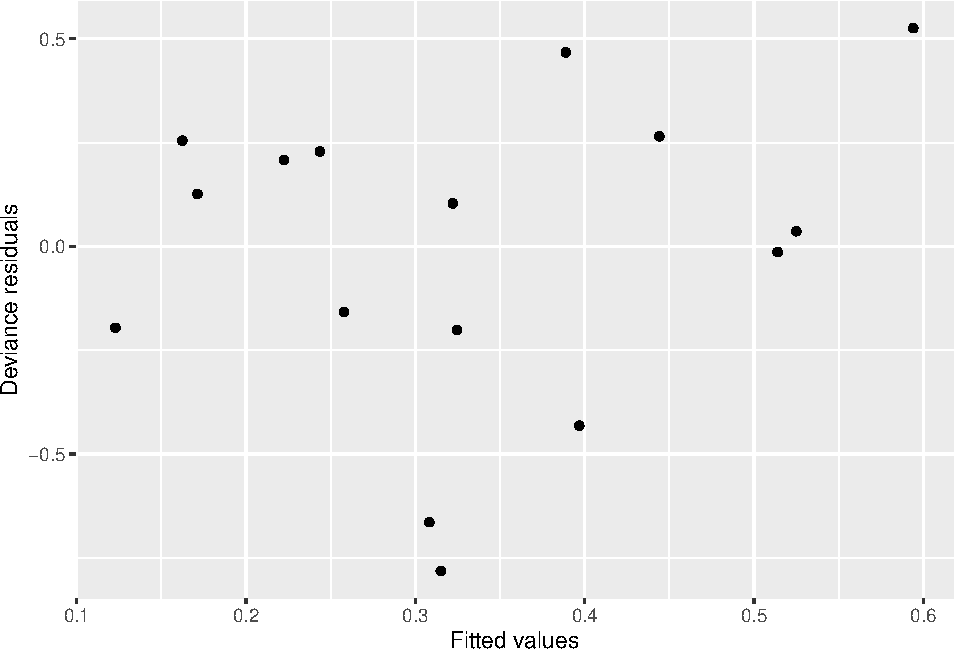
\includegraphics{3BinReg_files/figure-latex/unnamed-chunk-47-1.pdf}

\textbf{c)} Here is a code to produce a plot of fitted values for the 16
covariate patterns together with a saturated model (called frac) - on
the logit scale. How can you see from the dots for fitted values that we
are assuming an additive model on the logit scale (that is, the pattern
for each panel for logit fitted vs age is the same for each panel if we
have an additive model on the logit scale - you see that from the fitted
points)? Do you also see that for the observed values? Implication? Any
other observations?

\begin{Shaded}
\begin{Highlighting}[]
\FunctionTok{library}\NormalTok{(ggplot2)}
\NormalTok{frac}\OtherTok{=}\NormalTok{ds}\SpecialCharTok{$}\NormalTok{using}\SpecialCharTok{/}\NormalTok{(ds}\SpecialCharTok{$}\NormalTok{using}\SpecialCharTok{+}\NormalTok{ds}\SpecialCharTok{$}\NormalTok{notUsing)}
\NormalTok{logitdf}\OtherTok{=}\FunctionTok{data.frame}\NormalTok{(}\AttributeTok{lfitted=}\FunctionTok{qlogis}\NormalTok{(fit3add}\SpecialCharTok{$}\NormalTok{fitted),}\AttributeTok{lfrac=}\FunctionTok{qlogis}\NormalTok{(frac),}\AttributeTok{age=}\NormalTok{ds}\SpecialCharTok{$}\NormalTok{age,}\AttributeTok{wantsMore=}\NormalTok{ds}\SpecialCharTok{$}\NormalTok{wantsMore,}\AttributeTok{education=}\NormalTok{ds}\SpecialCharTok{$}\NormalTok{education)}
\FunctionTok{ggplot}\NormalTok{(logitdf,}\FunctionTok{aes}\NormalTok{(}\AttributeTok{x=}\NormalTok{age))}\SpecialCharTok{+}\FunctionTok{geom\_point}\NormalTok{(}\FunctionTok{aes}\NormalTok{(}\AttributeTok{y=}\NormalTok{lfrac,}\AttributeTok{colour=}\StringTok{"saturated"}\NormalTok{))}\SpecialCharTok{+}\FunctionTok{geom\_point}\NormalTok{(}\FunctionTok{aes}\NormalTok{(}\AttributeTok{y=}\NormalTok{lfitted,}\AttributeTok{colour=}\StringTok{"fitted"}\NormalTok{))}\SpecialCharTok{+}\FunctionTok{facet\_wrap}\NormalTok{(}\AttributeTok{facets=}\SpecialCharTok{\textasciitilde{}}\NormalTok{wantsMore}\SpecialCharTok{*}\NormalTok{education) }\SpecialCharTok{+} \FunctionTok{labs}\NormalTok{(}\AttributeTok{x =} \StringTok{"age"}\NormalTok{, }\AttributeTok{y =} \StringTok{""}\NormalTok{)}
\end{Highlighting}
\end{Shaded}

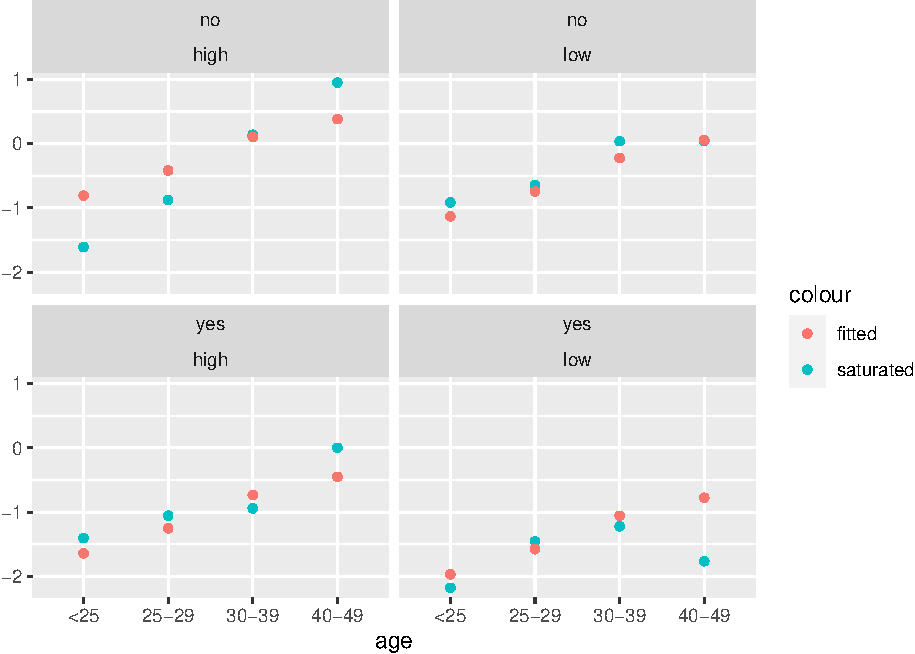
\includegraphics{3BinReg_files/figure-latex/unnamed-chunk-48-1.pdf}

To see what Rodríguez have found to be the best model, look at the
bottom of \url{http://data.princeton.edu/wws509/R/c3s6.html}.

\textbf{Note:} This exercise is based on the excellent notes of Germán
Rodríguez at Princeton, see in particular the R logs at
\url{http://data.princeton.edu/wws509/R/c3s1.html}.

\hypertarget{exam-questions}{%
\section{Exam questions}\label{exam-questions}}

For this module the following are exam questions to work with

\begin{itemize}
\tightlist
\item
  2012 --
  \href{https://www.math.ntnu.no/emner/TMA4315/Exam/GLMeksamen2012E.pdf}{Problem
  1}
\item
  2011 --
  \href{https://www.math.ntnu.no/emner/TMA4315/Exam/eksDes11e.pdf}{Problem
  1}
\end{itemize}

In addition these essay-type exam questions are closely related to this
module.

\hypertarget{december-2014}{%
\subsection{December 2014}\label{december-2014}}

There are two main asymptotic results that are behind essentially
everything we have done with respect to inference for generalized linear
models. These are

\begin{enumerate}
\def\labelenumi{\arabic{enumi}.}
\item
  asymptotic normality of maximum likelihood estimators (MLE), and
\item
  asymptotic result for likelihood ratio tests (LRT).
\end{enumerate}

State, describe and discuss the main assumptions behind these two
asymptotic results, how these results are used in practice to do
inference for parameters, testing various hypotheses and comparing
nested models, for logistic regression.

\hypertarget{december-2016}{%
\subsection{December 2016}\label{december-2016}}

We will consider (binomial or binary) logistic regression, where we have
independent observations
\[Y_i \sim \text{Binomial}(n_i,\pi_i) \text{ } i=1,\ldots,n\] so that
\[P(Y_i)=\binom{n_i}{y_i}\pi_i^{y_i}(1-\pi_i)^{n_i-y_i}, \text{ } y_i=0,1,\ldots, n_i\]
The linear predictor is \[ \eta_i={\bf x}_i^T\boldsymbol{\beta}\] and
\[ \pi_i=\frac{\exp(\eta_i)}{1+\exp(\eta_i)}\] or
\[ \text{logit}(\pi_i)=\eta_i.\] Here, \({\bf x}_i\) is a vector of the
\(p\) covariates for the \(i\)th observation \(y_i\) with size (number
of trials) \(n_i\), and \(\boldsymbol{\beta}\) is the vector of \(p\)
unknown regression coefficients.

Write an introduction to logistic regression and its practical usage,
for a student with a good background in statistics, but no knowledge
about Generalized Linear Models (GLM). Topics you may want to consider,
are

\begin{itemize}
\tightlist
\item
  When to use it? Underlying assumptions.
\item
  Parameter estimation, limiting results for the MLE, Fisher information
  and observed Fisher information, confidence intervals and hypothesis
  testing.
\item
  Output analysis, residual plots (when it is possible) and
  interpretation of the \(\boldsymbol{\beta}\)-coefficients
\item
  Deviance and its usage.
\end{itemize}

\hypertarget{r-packages}{%
\section{R packages}\label{r-packages}}

\begin{Shaded}
\begin{Highlighting}[]
\FunctionTok{install.packages}\NormalTok{(}\FunctionTok{c}\NormalTok{(}\StringTok{"tidyverse"}\NormalTok{,}
                   \StringTok{"investr"}\NormalTok{,}
                   \StringTok{"knitr"}\NormalTok{,}
                   \StringTok{"kableExtra"}\NormalTok{,}
                   \StringTok{"faraway"}\NormalTok{,}
                   \StringTok{"viridis"}\NormalTok{,}
                   \StringTok{"statmod"}\NormalTok{))}
\end{Highlighting}
\end{Shaded}

\hypertarget{references-for-further-reading}{%
\section{References for further
reading}\label{references-for-further-reading}}

\begin{itemize}
\tightlist
\item
  A. Agresti (2015): ``Foundations of Linear and Generalized Linear
  Models.'' Wiley.
\item
  A. J. Dobson and A. G. Barnett (2008): ``An Introduction to
  Generalized Linear Models'', Third edition.
\item
  J. Faraway (2015): ``Extending the Linear Model with R'', Second
  Edition. \url{http://www.maths.bath.ac.uk/~jjf23/ELM/}
\item
  P. McCullagh and J. A. Nelder (1989): ``Generalized Linear Models''.
  Second edition.
\end{itemize}

\end{document}
